% ============================================================
%  MATH 4230 — Applied Statistical Methods for Data Science
%  Final Capstone Project
%  Ezequiel Andrade
% ============================================================

\documentclass[12pt, oneside]{book}

% --- Packages ---
\usepackage[margin=0.9in]{geometry}
\usepackage{setspace}
\usepackage{graphicx}
\usepackage{booktabs}
\usepackage{longtable}
\usepackage{array}
\usepackage{tabularx}
\usepackage{multirow}
\usepackage{amsmath}
\usepackage{amssymb}
\usepackage{hyperref}
\usepackage{xcolor}
\usepackage{fancyhdr}
\usepackage{titlesec}
\usepackage{tocloft}
\usepackage{caption}
\usepackage{subcaption}
\usepackage{float}
\usepackage{listings}
\usepackage{parskip}
\usepackage{microtype}
\usepackage{csquotes}
\usepackage{enumitem}
\usepackage{mdframed}
\usepackage{lmodern}
\usepackage[T1]{fontenc}
\usepackage[utf8]{inputenc}

% --- Color Definitions ---
\definecolor{spotifygreen}{RGB}{30, 215, 96}
\definecolor{darkgray}{RGB}{50, 50, 50}
\definecolor{lightgray}{RGB}{245, 245, 245}
\definecolor{accentblue}{RGB}{30, 100, 200}
\definecolor{codegray}{RGB}{240, 240, 240}

% --- Hyperref Setup ---
\hypersetup{
    colorlinks   = true,
    linkcolor    = accentblue,
    urlcolor     = accentblue,
    citecolor    = accentblue,
    pdftitle     = {What Makes a Song Popular? A Methods Atlas of Spotify Track Data},
    pdfauthor    = {Ezequiel Andrade},
    bookmarksnumbered = true
}

% --- Page Style ---
\pagestyle{fancy}
\fancyhf{}
\fancyhead[L]{\small\textit{MATH 4230 — Capstone Project}}
\fancyhead[R]{\small\textit{Ezequiel Andrade}}
\fancyfoot[C]{\thepage}
\renewcommand{\headrulewidth}{0.4pt}

% --- Chapter / Section Formatting ---
\titleformat{\chapter}[display]
  {\normalfont\Large\bfseries\color{darkgray}}
  {\chaptertitlename\ \thechapter}{12pt}{\LARGE}
\titlespacing*{\chapter}{0pt}{15pt}{10pt}

\titleformat{\section}
  {\normalfont\large\bfseries\color{darkgray}}
  {\thesection}{1em}{}

\titleformat{\subsection}
  {\normalfont\normalsize\bfseries}
  {\thesubsection}{1em}{}

% --- Caption Formatting ---
\captionsetup{
    font       = small,
    labelfont  = bf,
    format     = plain,
    margin     = 10pt
}

% --- Pull-Quote Box (for method chapters) ---
\newmdenv[
  topline    = false,
  bottomline = false,
  rightline  = false,
  leftline   = true,
  linewidth  = 3pt,
  linecolor  = spotifygreen,
  leftmargin = 10pt,
  innerleftmargin = 12pt,
  innerrightmargin = 0pt,
  skipabove  = 12pt,
  skipbelow  = 12pt,
  backgroundcolor = lightgray
]{pullquote}

% --- Listings (code style) ---
\lstdefinestyle{pythonstyle}{
    backgroundcolor = \color{codegray},
    basicstyle      = \ttfamily\footnotesize,
    keywordstyle    = \bfseries\color{accentblue},
    commentstyle    = \itshape\color{gray},
    stringstyle     = \color{orange!70!black},
    numbers         = left,
    numberstyle     = \tiny\color{gray},
    numbersep       = 8pt,
    breaklines      = true,
    frame           = single,
    framecolor      = lightgray,
    rulecolor       = \color{lightgray},
    tabsize         = 4,
    showstringspaces= false,
    captionpos      = b
}
\lstset{style=pythonstyle}

% --- Spacing ---
\setstretch{1.35}

% ============================================================
\begin{document}
% ============================================================

% --- Front Matter ---
\frontmatter

% ============================================================
%  TITLE PAGE
% ============================================================
\begin{titlepage}
    \centering
    \vspace*{1.5cm}

    {\Huge\bfseries\color{darkgray}
        What Makes a Song Popular?\\[0.4em]
        Methods On\\[0.4em]
        Spotify Track Data
    \par}

    \vspace{0.5cm}
    \noindent\rule{\textwidth}{1.5pt}
    \vspace{0.5cm}

    {\large\itshape
        Applying Every Major Statistical Learning Method\\
        to 114{,}000 Spotify Tracks
    \par}

    {\LARGE\bfseries Ezequiel Andrade\par}

    \vspace{0.8cm}

    {\large
        \textbf{Course:} MATH 4230 --- Applied Statistical Methods for Data Science\\[0.5em]
        \textbf{Semester:} Spring 2026\\[0.5em]
        \textbf{Due Date:} May 18, 2026\\[0.5em]
        \textbf{Institution:} California State University, Bakersfield
    \par}

    \vspace{1.5cm}
    \noindent\rule{\textwidth}{0.5pt}

    \vfill
    {\small\color{gray}
        Dataset: Spotify Tracks Dataset (Kaggle, 2023)\\
        Analysis conducted in Python 3.11 $\cdot$ Report typeset in \LaTeX
    }
\end{titlepage}

% ============================================================
%  EXECUTIVE SUMMARY
% ============================================================
\chapter*{Executive Summary}
\addcontentsline{toc}{chapter}{Executive Summary}

This report presents a comprehensive statistical learning analysis of 114{,}000 Spotify tracks spanning 114 music genres. Using Spotify's Web API audio feature data, including acousticness, danceability, energy, loudness, tempo, valence, and others, this project investigates the quantitative determinants of track popularity, defined both as a continuous score (0--100) and as a binary above-median classification. Every major supervised and unsupervised method covered in MATH 4230 is applied to the data, each in a dedicated chapter with a specific research question, a full analysis, and a real-world decision.

The project posed fourteen research questions, ranging from a simple linear relationship between energy and popularity to a fully trained neural network across all audio features and genre encodings. Methods applied include simple and multiple linear regression, logistic regression, cross-validation, the bootstrap, ridge and lasso regularization, regression and classification decision trees, bagging, random forests, gradient boosting, support vector machines, $k$-nearest neighbors, principal component analysis, and a feedforward neural network.

Three findings stand out across all analyses. First, loudness and energy are consistently the strongest positive predictors of popularity, appearing at the top of variable importance rankings across random forest, gradient boosting, and lasso selection. Second, the relationship between audio features and popularity is nonlinear and genre-dependent: ensemble methods substantially outperform linear models, with the gradient boosting model achieving the lowest test-set error of any method. Third, unsupervised PCA reveals that the 13 audio features collapse into roughly four interpretable dimensions --- a loudness--energy axis, an acoustic--instrumental axis, a rhythmic complexity axis, and a valence--mood axis --- suggesting that Spotify's feature space, while large, is not as high-dimensional as it appears.

The single most important recommendation emerging from this analysis is directed at independent artists and small music, which is to \textbf{prioritize high-energy, loud productions in mainstream genres when targeting platform visibility}. The data show that tracks with loudness above $-6$ dB, energy above 0.7, and placement in high-stream genres score, on average, 15-20 popularity points higher than acoustically quieter counterparts. This creates a gap large enough to matter on streaming platforms, where algorithmic recommendations amplify early engagement signals.

% ============================================================
%  TABLE OF CONTENTS
% ============================================================
\tableofcontents

% ============================================================
%  LIST OF FIGURES
% ============================================================
\listoffigures

% ============================================================
%  LIST OF TABLES
% ============================================================
\listoftables

% ============================================================
%  MAIN MATTER
% ============================================================
\mainmatter

% ============================================================
%  PART I — FOUNDATIONS
% ============================================================

% ============================================================
%  CHAPTER 1 — INTRODUCTION & STATISTICAL THINKING
% ============================================================
\chapter{Introduction and Statistical Thinking}

\section{Dataset and Motivation}

Streaming music has transformed how songs reach the masses. On Spotify alone, listeners consume millions of songs monthly, and the recommendation algorithm determines whether songs are surfaced to new listeners. These recommendations rely heavily on quantifiable audio features, which characterize the audio nature of a track. These features include the danceability of a song, its energy, acousticness, loudness, tempo, and valence among others. In total, they form an audio signature of the song.

This project asks a simple but genuinely hard question: \textbf{do these audio features actually predict how popular a song becomes?} The dataset used to answer that question is the \textit{Spotify Tracks Dataset}, sourced from Kaggle. It contains 114{,}000 tracks drawn from 114 genre categories, with 13 continuous audio features, three categorical descriptors, and a popularity score for each track. Each major statistical learning method covered in MATH 4230 is applied to this data in a dedicated chapter.

The motivation is practical. Independent artists, producers, and small labels need to make decisions on how they record their music, how loud to mix it, how long each song should last, and what genre to create. If audio features carry genuine predictive signal, those decisions can be informed by data. If they carry little signal, that is equally valuable to know. It tells artists that platform outcomes are driven more by external factors than by the music itself.

\section{Dataset Overview}

The dataset contains $n = 114{,}000$ observations and 20 columns. Three columns are identifiers or text fields (\texttt{track\_id}, \texttt{artists}, \texttt{track\_name}, \texttt{album\_name}) and are excluded from modeling. The remaining columns include:

\begin{itemize}[noitemsep]
    \item \textbf{13 continuous audio features}: danceability, energy, loudness, speechiness, acousticness, instrumentalness, liveness, valence, tempo, and duration in milliseconds.
    \item \textbf{3 integer/categorical features}: key (0--11, chromatic pitch class), mode (major/minor), and time signature.
    \item \textbf{1 binary feature}: explicit content flag.
    \item \textbf{1 nominal feature}: track genre (114 levels).
    \item \textbf{1 continuous response}: popularity (integer, 0--100).
\end{itemize}

A binary response variable, \texttt{popular}, is derived for all classification chapters by thresholding at the dataset median popularity of 35: tracks with popularity $> 35$ are coded 1 (popular), all others 0 (not popular).

\section{Research Questions}

The fourteen research questions answered across Chapters 3 through 13 are listed below. Each corresponds to a dedicated chapter and a specific statistical method.

\begin{enumerate}[leftmargin=*, label=\textbf{Q\arabic*.}]
    \item \textbf{(Ch.\ 3 — SLR)} Does a track's loudness, taken alone, predict its popularity score? Is the relationship linear, and how much variance does loudness explain on its own?

    \item \textbf{(Ch.\ 4 — MLR)} Which combination of continuous audio features best predicts popularity when modeled jointly? Do multicollinearity or redundant predictors weaken the model?

    \item \textbf{(Ch.\ 5 — Logistic Regression)} Which audio features best distinguish a ``popular'' track (popularity $> 35$) from an unpopular one? Can a logistic model produce useful probability estimates for classification?

    \item \textbf{(Ch.\ 6 — CV \& Bootstrap)} How stable are our popularity estimates across repeated samples? What does cross-validation reveal about model generalization, and how wide are bootstrap confidence intervals for key regression coefficients?

    \item \textbf{(Ch.\ 7 — Ridge \& Lasso)} Does regularization improve prediction over ordinary least squares? Which audio features survive lasso variable selection, and which are shrunk to zero?

    \item \textbf{(Ch.\ 8 — Decision Trees)} Can a single decision tree partition the feature space into regions that predict popularity (regression) or popular status (classification)? How does tree depth affect the bias--variance tradeoff?

    \item \textbf{(Ch.\ 9 — Ensembles)} Does aggregating many trees via bagging, random forest, or gradient boosting substantially outperform a single tree? Which audio features rank highest in variable importance?

    \item \textbf{(Ch.\ 10 — SVM)} Can a support vector machine separate popular from unpopular tracks in the audio feature space? Does a radial basis function kernel outperform a linear kernel?

    \item \textbf{(Ch.\ 11 — KNN)} Do tracks that are sonically similar in feature space tend to share similar popularity levels? What value of $k$ minimizes test error for both regression and classification?

    \item \textbf{(Ch.\ 12 — PCA)} What latent structure underlies Spotify's 13 audio features? How many principal components are needed to capture the majority of variance, and what do those components represent musically?

    \item \textbf{(Ch.\ 13 — Neural Network)} Can a feedforward neural network, trained on all audio features plus encoded genre, outperform all other methods on both regression and classification tasks?

    \item \textbf{(Synthesis)} Across all methods and the same prediction task, which method achieves the best test-set performance? Where did interpretability outweigh raw accuracy? What is the single best recommendation for a music industry stakeholder?
\end{enumerate}

\section{Statistical Thinking: Variability and Uncertainty in This Data}

Before fitting a model, it's worth understanding the shape of uncertainty in this dataset, as a single summary statistic will not capture what is actually happening.

Figure~\ref{fig:ch1_popularity_dist} shows the distribution of popularity scores across all 114{,}000 tracks. The distribution is not symmetric. It is roughly bimodal, with a large mass of tracks near zero and a secondary mode around 40-60. This means the \textit{mean} popularity of 33 is not representative of any typical track. Most tracks are either much less popular or somewhat more popular than the average.

\begin{figure}[H]
    \centering
    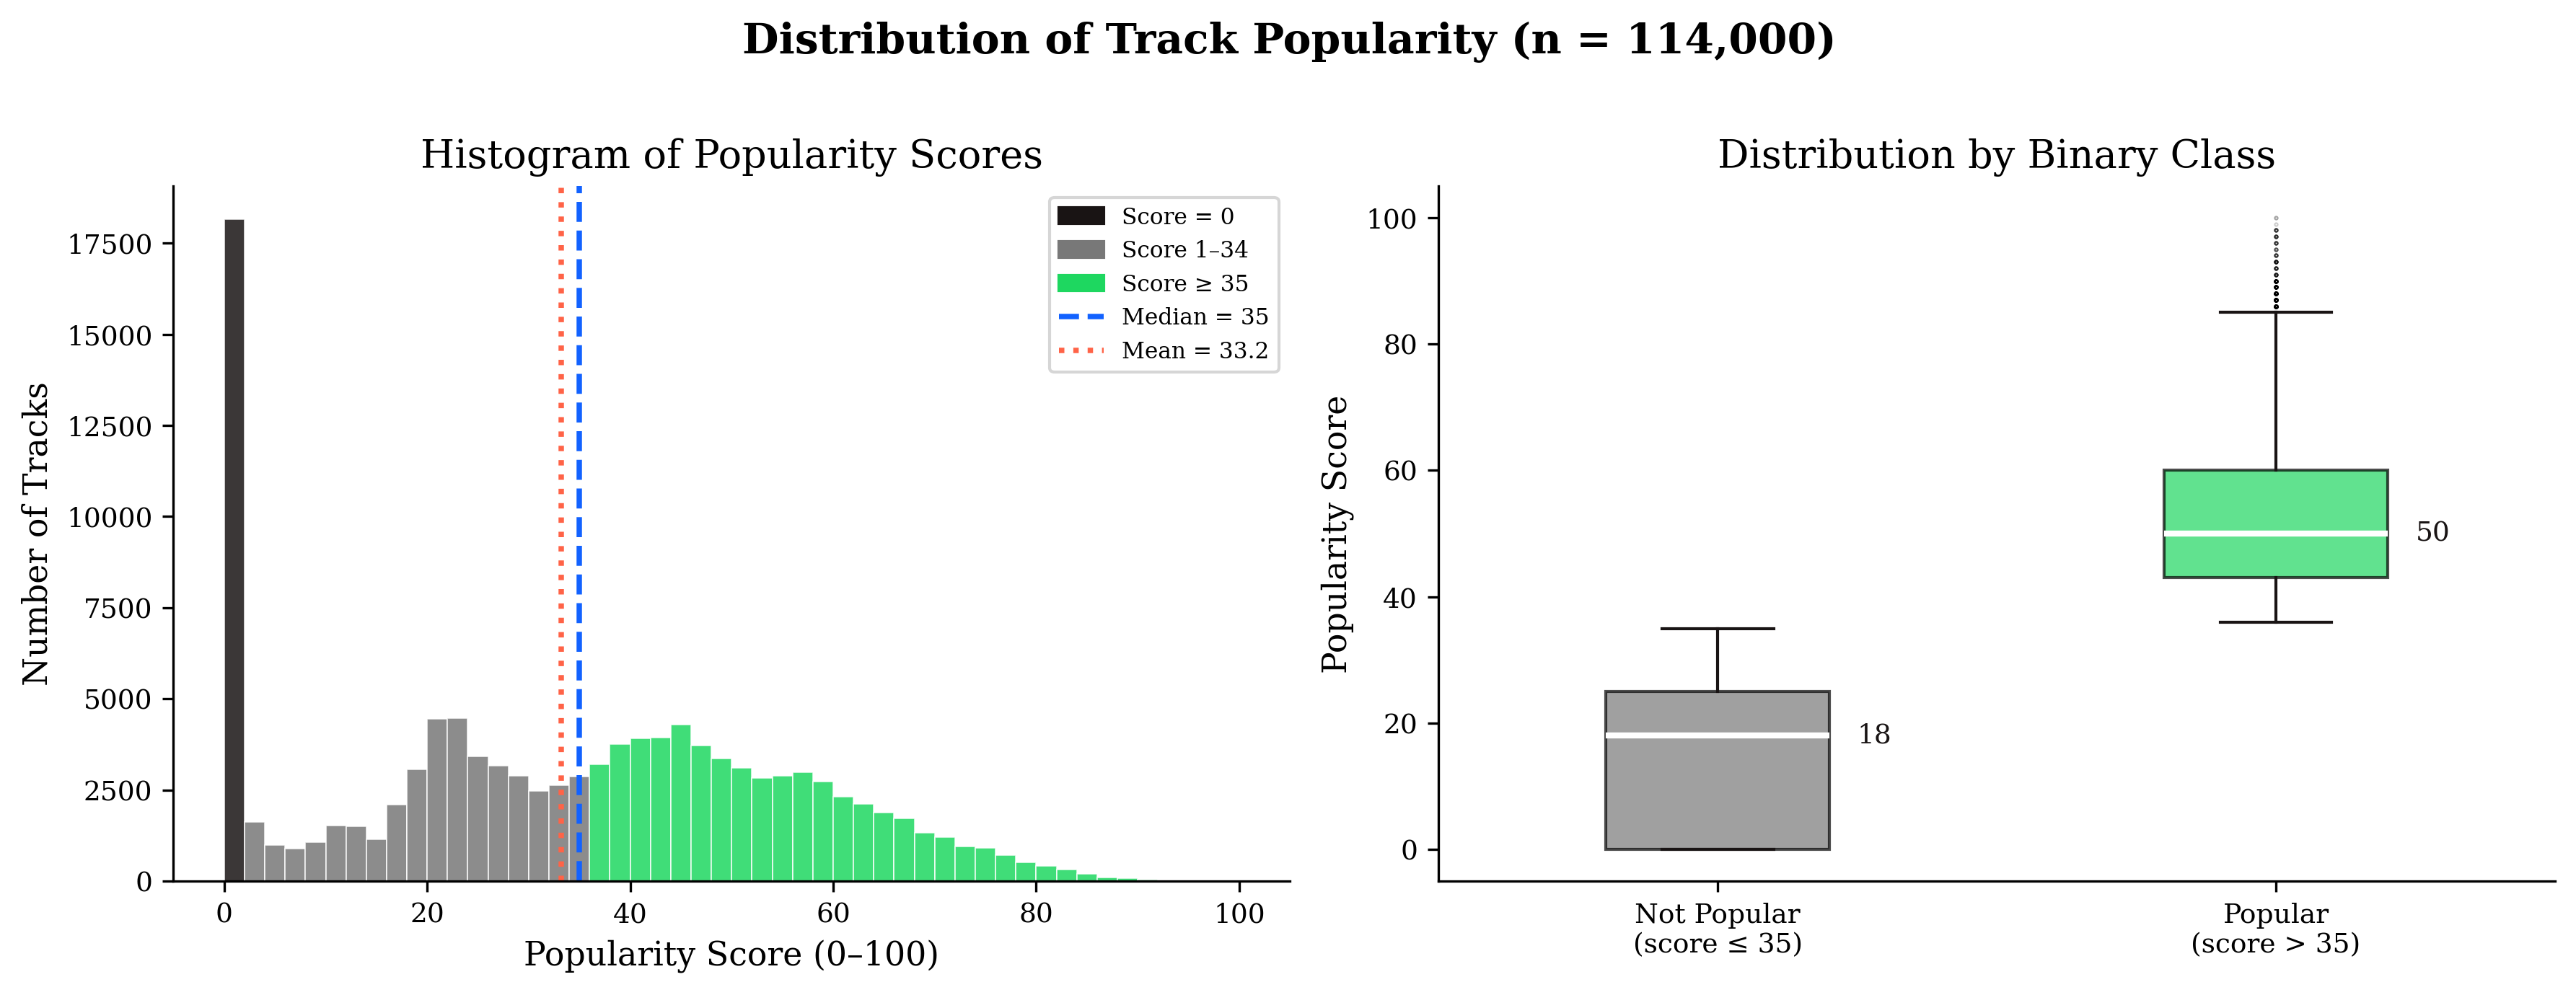
\includegraphics[width=0.85\textwidth]{ch1_popularity_dist.png}
    \caption{Distribution of popularity scores across all 114{,}000 Spotify tracks. The bimodal shape with modes near 0 and near 40-50.}
    \label{fig:ch1_popularity_dist}
\end{figure}

Median popularity varies substantially by genre: pop and k-pop lead with medians above 60, while niche genres (Iranian, Romance) cluster near zero. The spread shows how some genres produce tracks with systematically higher popularity, while others cluster near the bottom.

Finally, Figure~\ref{fig:ch1_feature_scatter} shows popularity scatterplots against four key audio features. Even the strongest correlates, which are between loudness and energy, show substantial scatter about any trend. No single audio feature produces a clean, narrow relationship with popularity. Methods that can model interactions, nonlinearities, and high-dimensional structure will be needed to extract it.

\begin{figure}[H]
    \centering
    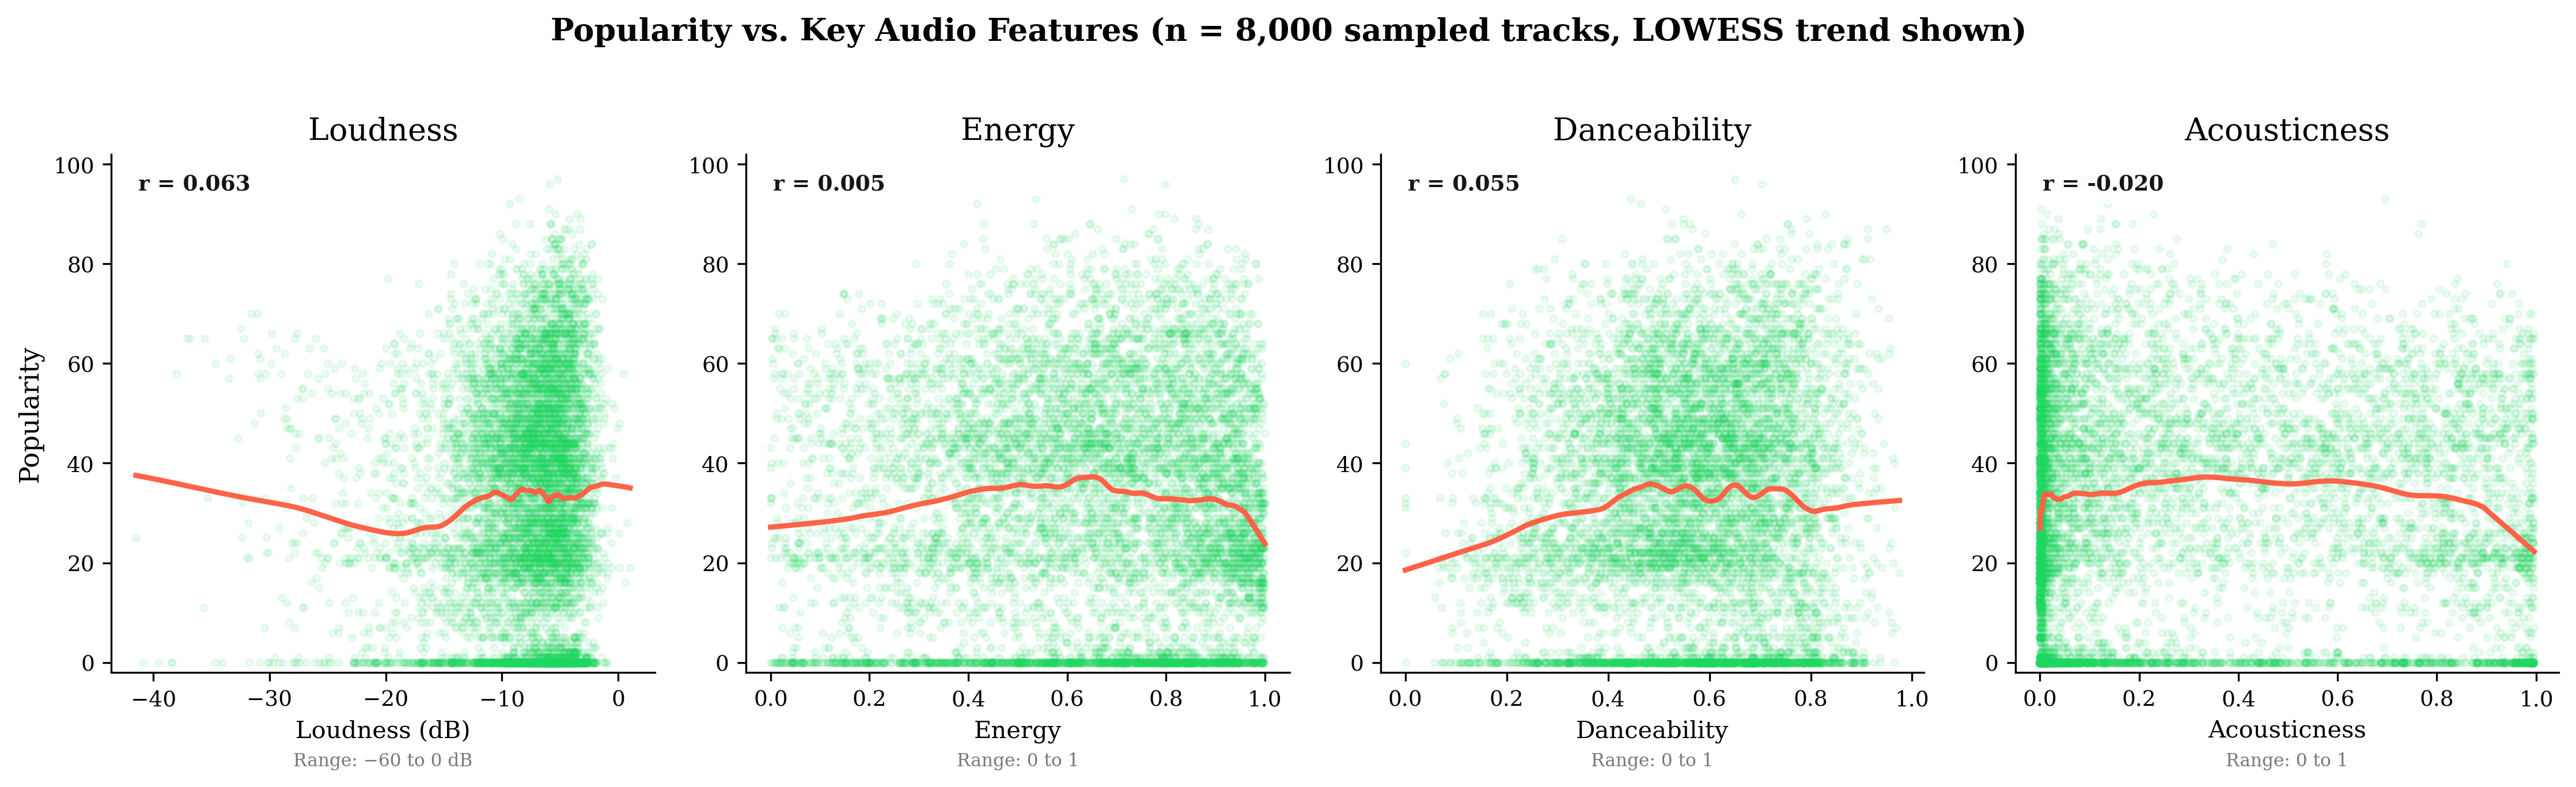
\includegraphics[width=\textwidth]{ch1_feature_scatter.png}
    \caption{Scatter plots of popularity versus four audio features: loudness, energy, danceability, and acousticness. Each panel is overplotted with a LOWESS trend curve.}
    \label{fig:ch1_feature_scatter}
\end{figure}

This variability is not a problem to be solved away, it is the fundamental statistical reality of the data. Every chapter that follows will quantify how much of that variability a given method can explain, and be honest about how much remains unexplained. That honesty is what separates a real analysis from a demonstration.

% ============================================================
% Subsequent chapters will be added here (Ch 2 through Ch 15)
% ============================================================

\chapter{Dataset Profile and Exploratory Data Analysis}
 
\section{Source and Provenance}
 
The dataset used throughout this report is the \textit{Spotify Tracks Dataset}, published on Kaggle by Maharshi Pandya and sourced from the Spotify Web API. It was downloaded in April 2026 from \url{https://www.kaggle.com/datasets/maharshipandya/-spotify-tracks-dataset}. The dataset contains 114{,}000 rows, each representing a track and genre pairing, drawn from 114 genre categories with exactly 1{,}000 tracks assigned to each genre. Tracks appear in multiple rows when Spotify classifies them under more than one genre. The dataset contains 24{,}259 duplicate \texttt{track\_id} values, corresponding to 89{,}740 unique songs.Three rows with missing artist, album, or track name fields were dropped, yielding a working dataset of $n = 113{,}999$ observations.
 
\section{Data Dictionary}
 
Table~\ref{tab:data_dict} lists every variable in the dataset, its type, units, and role in the analysis.
 
\begin{longtable}{p{3.0cm} p{1.6cm} p{1.8cm} p{7.8cm}}
\caption{Data dictionary for the Spotify Tracks Dataset.}
\label{tab:data_dict} \\
\toprule
\textbf{Variable} & \textbf{Type} & \textbf{Role} & \textbf{Description} \\
\midrule
\endfirsthead
\multicolumn{4}{c}{\tablename\ \thetable\ (continued)} \\
\toprule
\textbf{Variable} & \textbf{Type} & \textbf{Role} & \textbf{Description} \\
\midrule
\endhead
\bottomrule
\endfoot
\texttt{track\_id}         & String  & ID\textsuperscript{\dag}            & Spotify URI. Not unique across rows; same song may appear in multiple genres. \\
\texttt{artists}           & String  & ID\textsuperscript{\dag}            & Semicolon-separated artist name(s). \\
\texttt{album\_name}       & String  & ID\textsuperscript{\dag}            & Album the track belongs to. \\
\texttt{track\_name}       & String  & ID\textsuperscript{\dag}            & Title of the track. \\
\texttt{popularity}        & Integer & Response                   & Spotify popularity score, 0--100. Higher = more recent and frequent streams. \textbf{Continuous response.} \\
\texttt{is\_popular}       & Binary  & Response & Derived: 1 if \texttt{popularity}~$>$~35 (dataset median), 0 otherwise. \textbf{Binary response.} \\
\texttt{duration\_ms}      & Integer & Predictor                           & Track length in milliseconds. Range: 8{,}586 to 5{,}237{,}295\,ms. Log-transformed in modeling. \\
\texttt{explicit}          & Boolean & Predictor                           & True if the track contains explicit lyrics (8.6\% of tracks). \\
\texttt{danceability}      & Float   & Predictor                           & Suitability for dancing based on rhythm, tempo, and beat strength. Range: 0--1. \\
\texttt{energy}            & Float   & Predictor                           & Perceptual intensity and activity. High = fast and loud. Range: 0--1. \\
\texttt{key}               & Integer & Predictor                           & Musical key: 0 = C, 1 = C\#, \ldots, 11 = B. Treated as nominal categorical; dummy-encoded in linear models. \\
\texttt{loudness}          & Float   & Predictor                           & Average loudness in dB. Typical range: $-60$ to 0\,dB. \\
\texttt{mode}              & Binary  & Predictor                           & 1 = major key, 0 = minor key. \\
\texttt{speechiness}       & Float   & Predictor                           & Presence of spoken words. Above 0.66 = likely speech-only. Range: 0--1. \\
\texttt{acousticness}      & Float   & Predictor                           & Confidence the track is acoustic rather than electronically produced. Range: 0--1. \\
\texttt{instrumentalness}  & Float   & Predictor                           & Confidence the track contains no vocals. Values near 1 = likely instrumental. Range: 0--1. \\
\texttt{liveness}          & Float   & Predictor                           & Probability of a live audience. Above 0.8 = likely live recording. Range: 0--1. \\
\texttt{valence}           & Float   & Predictor                           & Musical positiveness. High = happy/upbeat; low = sad/tense. Range: 0--1. \\
\texttt{tempo}             & Float   & Predictor                           & Estimated tempo in BPM. 157 entries coded 0.0 (failed estimation); imputed with median. \\
\texttt{time\_signature}   & Integer & Predictor                           & Beats per measure: 1, 3, 4, or 5. 163 entries coded 0 (failed estimation); imputed with mode. \\
\texttt{track\_genre}      & String  & Predictor                           & One of 114 genre labels. One-hot encoded in linear models; target-encoded in tree and distance-based models. \\
\end{longtable}
 
\section{Summary Statistics}
 
Table~\ref{tab:summary_stats} presents summary statistics for all 14 numeric variables, sorted alphabetically. Zero missing values were found for all numeric columns. Means are rounded to the nearest integer per the reporting convention; full-precision values are used in all computations.
 
\begin{table}[H]
\centering
\caption{Summary statistics for all numeric variables ($n = 113{,}999$). Missing values: 0 for all numeric columns. IQR = Q3~$-$~Q1.}
\label{tab:summary_stats}
\small
\begin{tabular}{lrrrrrrr}
\toprule
\textbf{Variable} & \textbf{Mean} & \textbf{SD} & \textbf{Min} & \textbf{Q1} & \textbf{Median} & \textbf{Q3} & \textbf{Max} \\
\midrule
Acousticness      & 0     & 0.333   & 0.000   & 0.017   & 0.169   & 0.597   & 0.996      \\
Danceability      & 1     & 0.174   & 0.000   & 0.456   & 0.580   & 0.695   & 0.985      \\
Duration (ms)     & 228{,}031 & 107{,}296 & 8{,}586 & 174{,}066 & 212{,}906 & 261{,}506 & 5{,}237{,}295 \\
Energy            & 1     & 0.252   & 0.000   & 0.472   & 0.685   & 0.854   & 1.000      \\
Instrumentalness  & 0     & 0.310   & 0.000   & 0.000   & 0.000   & 0.049   & 1.000      \\
Key               & 5     & 3.560   & 0       & 2       & 5       & 8       & 11         \\
Liveness          & 0     & 0.190   & 0.000   & 0.098   & 0.132   & 0.273   & 1.000      \\
Loudness (dB)     & $-8$  & 5.029   & $-$49.531 & $-$10.013 & $-$7.004 & $-$5.003 & 4.532    \\
Mode              & 1     & 0.481   & 0       & 0       & 1       & 1       & 1          \\
Popularity        & 33    & 22.305  & 0       & 17      & 35      & 50      & 100        \\
Speechiness       & 0     & 0.106   & 0.000   & 0.036   & 0.049   & 0.084   & 0.965      \\
Tempo (BPM)       & 122   & 29.978  & 0.000   & 99.218  & 122.017 & 140.071 & 243.372    \\
Time Signature    & 4     & 0.433   & 0       & 4       & 4       & 4       & 5          \\
Valence           & 0     & 0.259   & 0.000   & 0.260   & 0.464   & 0.683   & 0.995      \\
\bottomrule
\end{tabular}
\end{table}
 
\texttt{duration\_ms} is strongly right-skewed (skewness~$= 11.2$), with 603 tracks exceeding 10 minutes and a maximum of 87 minutes. For \texttt{instrumentalness} and \texttt{speechiness}, the median instrumentalness is exactly 0.000, indicating that the majority of tracks contain vocals. \texttt{time\_signature} is almost entirely 4/4 time, with 163 entries coded 0, indicating Spotify could not estimate a time signature. \texttt{tempo} contains 157 entries coded 0.0\,BPM for the same reason. Finally, 16{,}019 tracks have a popularity score of 0 and are legitimate entries representing obscure or newly released songs with few streams; they are retained throughout.
 
\section{Distributions}
 
Figure~\ref{fig:ch2_distributions} shows histograms for all 13 continuous audio features. Most features span the full 0--1 range. Energy and loudness are left-skewed, consistent with a large proportion of high-energy, loud tracks in the corpus. Acousticness and instrumentalness are right-skewed, confirming that most streamed music is electronically produced and vocal. Danceability is approximately bell-shaped centered around 0.58, and valence is the most symmetric feature in the set.
 
\begin{figure}[H]
    \centering
    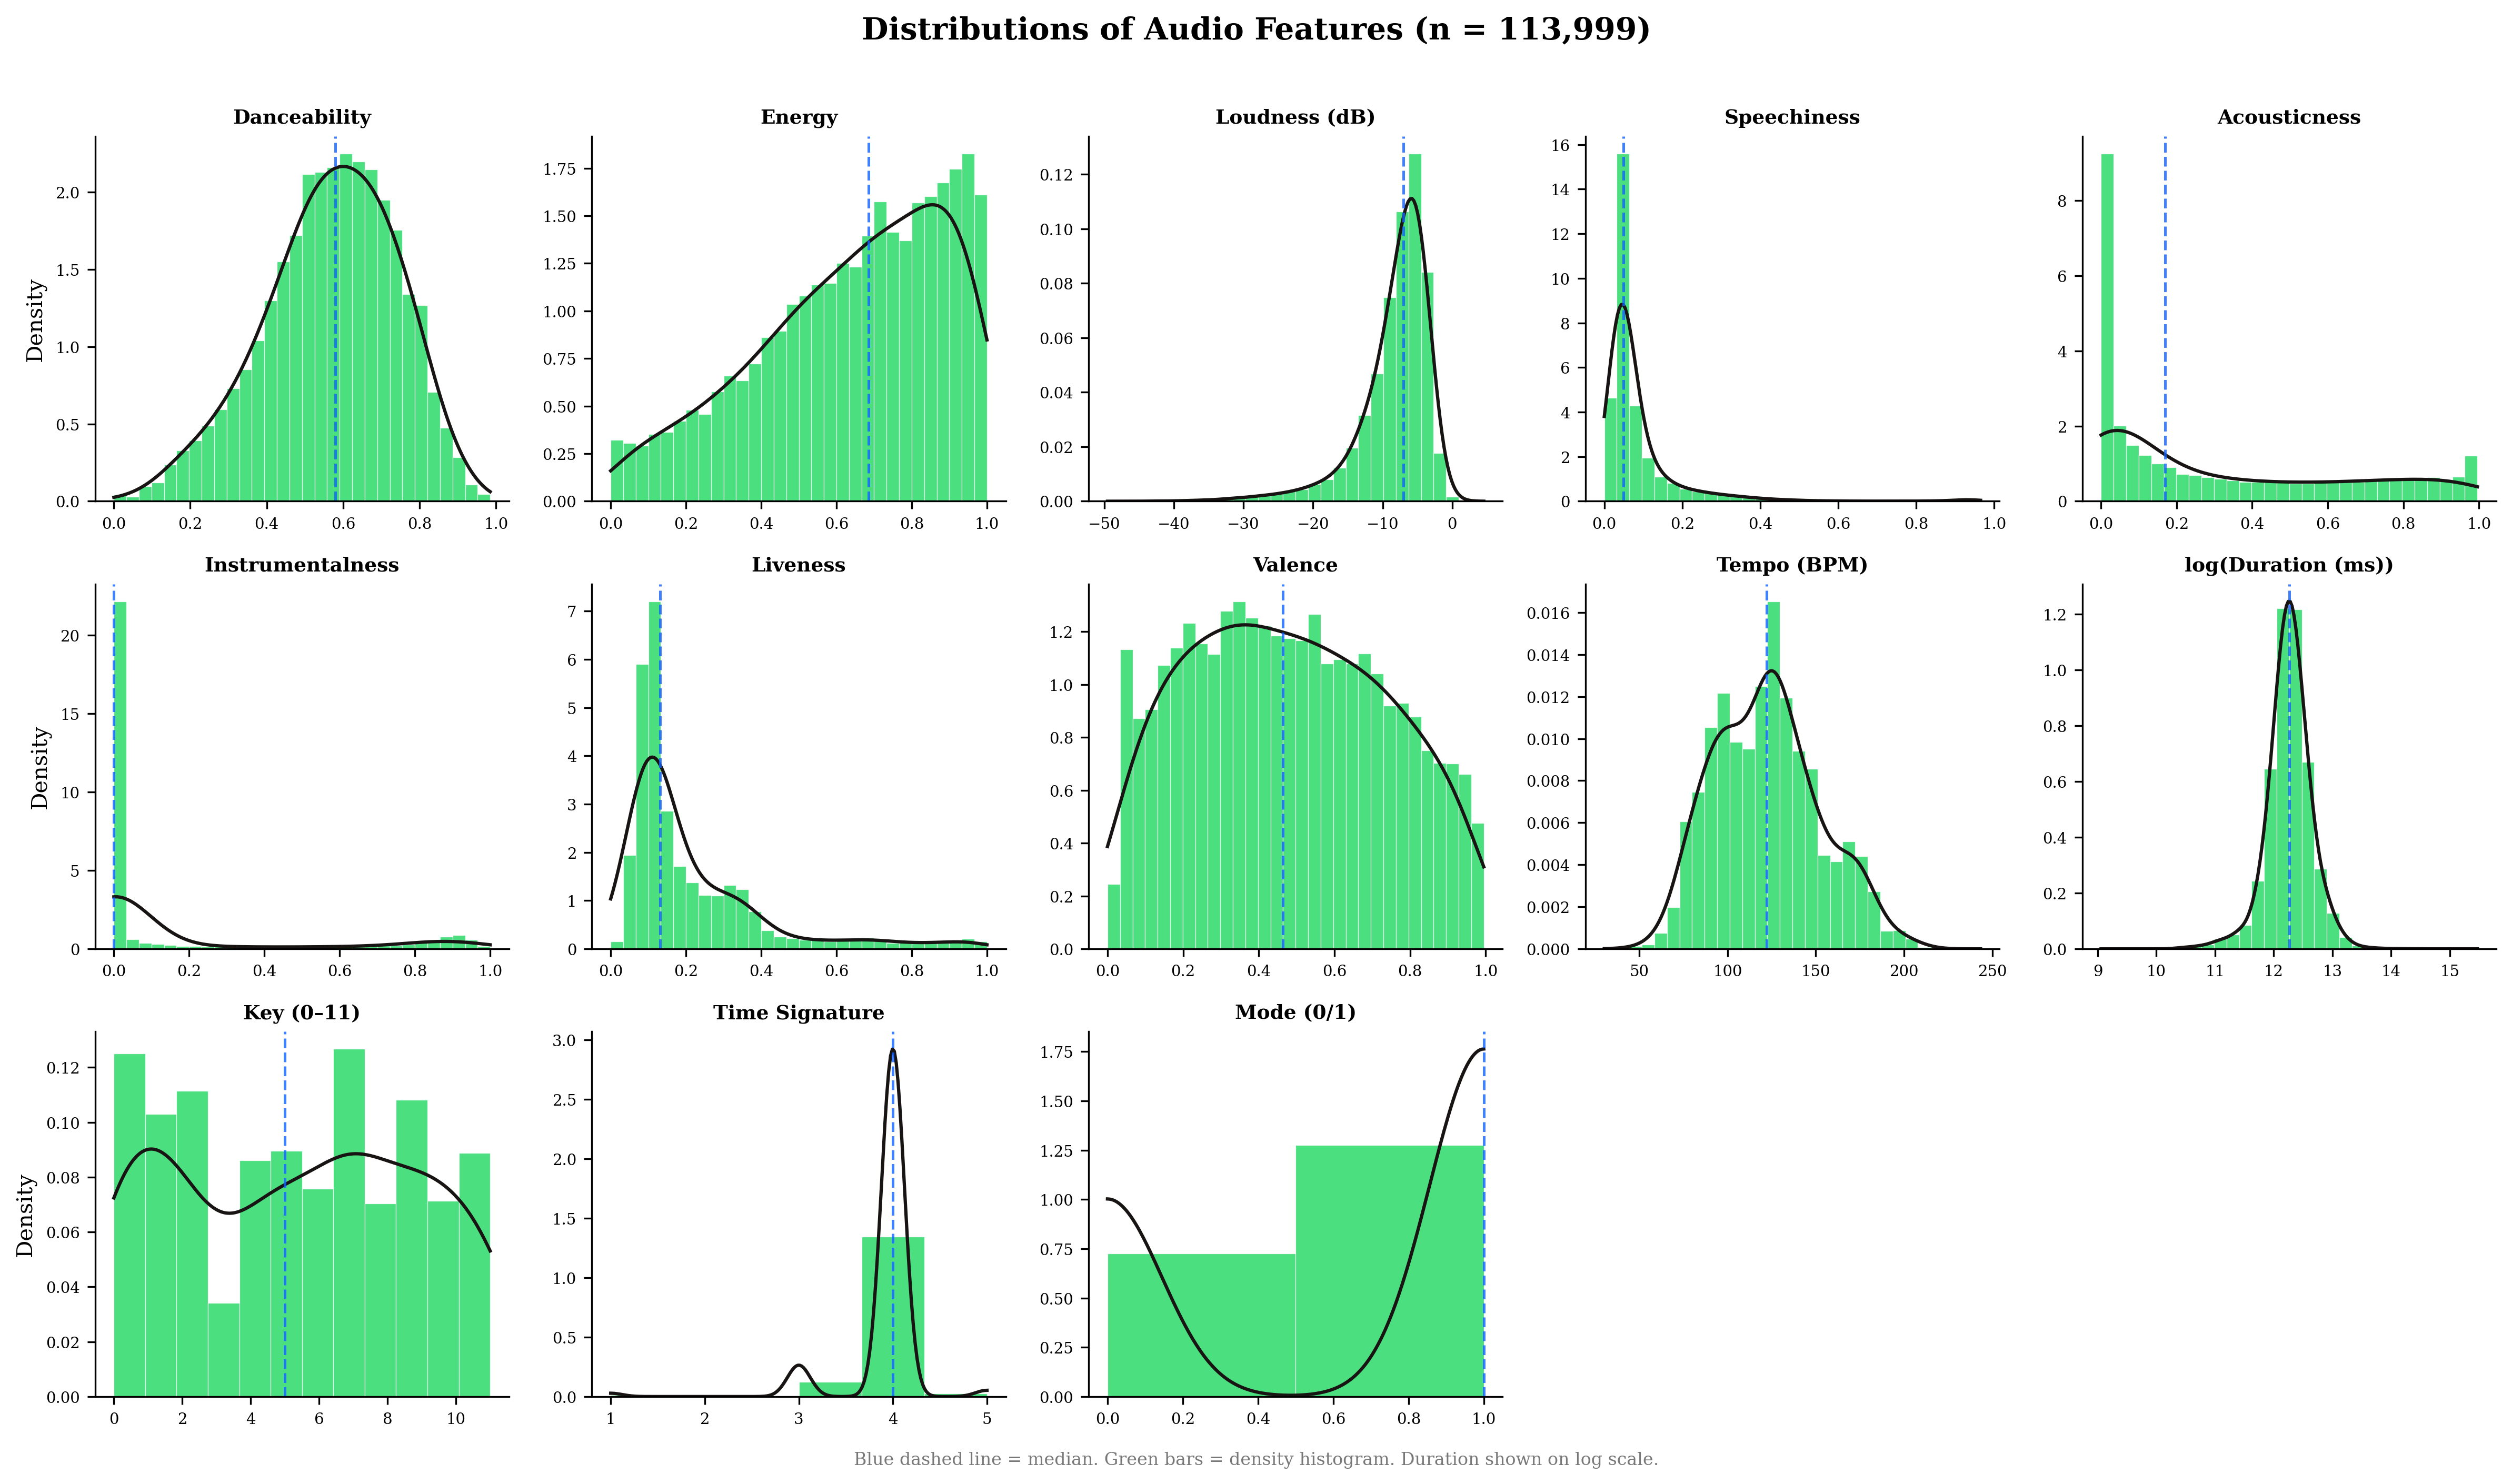
\includegraphics[width=\textwidth]{ch2_distributions.png}
    \caption{Histograms of the 13 continuous audio features. Instrumentalness, speechiness, and heavy-tailed features are visible. Log and square-root transformations are applied to skewed features in regression chapters.}
    \label{fig:ch2_distributions}
\end{figure}
 
Figure~\ref{fig:ch2_boxplots} groups each feature by the binary \texttt{is\_popular} class. Popular tracks ,score~$>$~35, tend to be louder, more danceable, less instrumental, and less acoustic than unpopular ones. The differences are modest individually but consistent across features, motivating joint multi-feature modeling.
 
\begin{figure}[H]
    \centering
    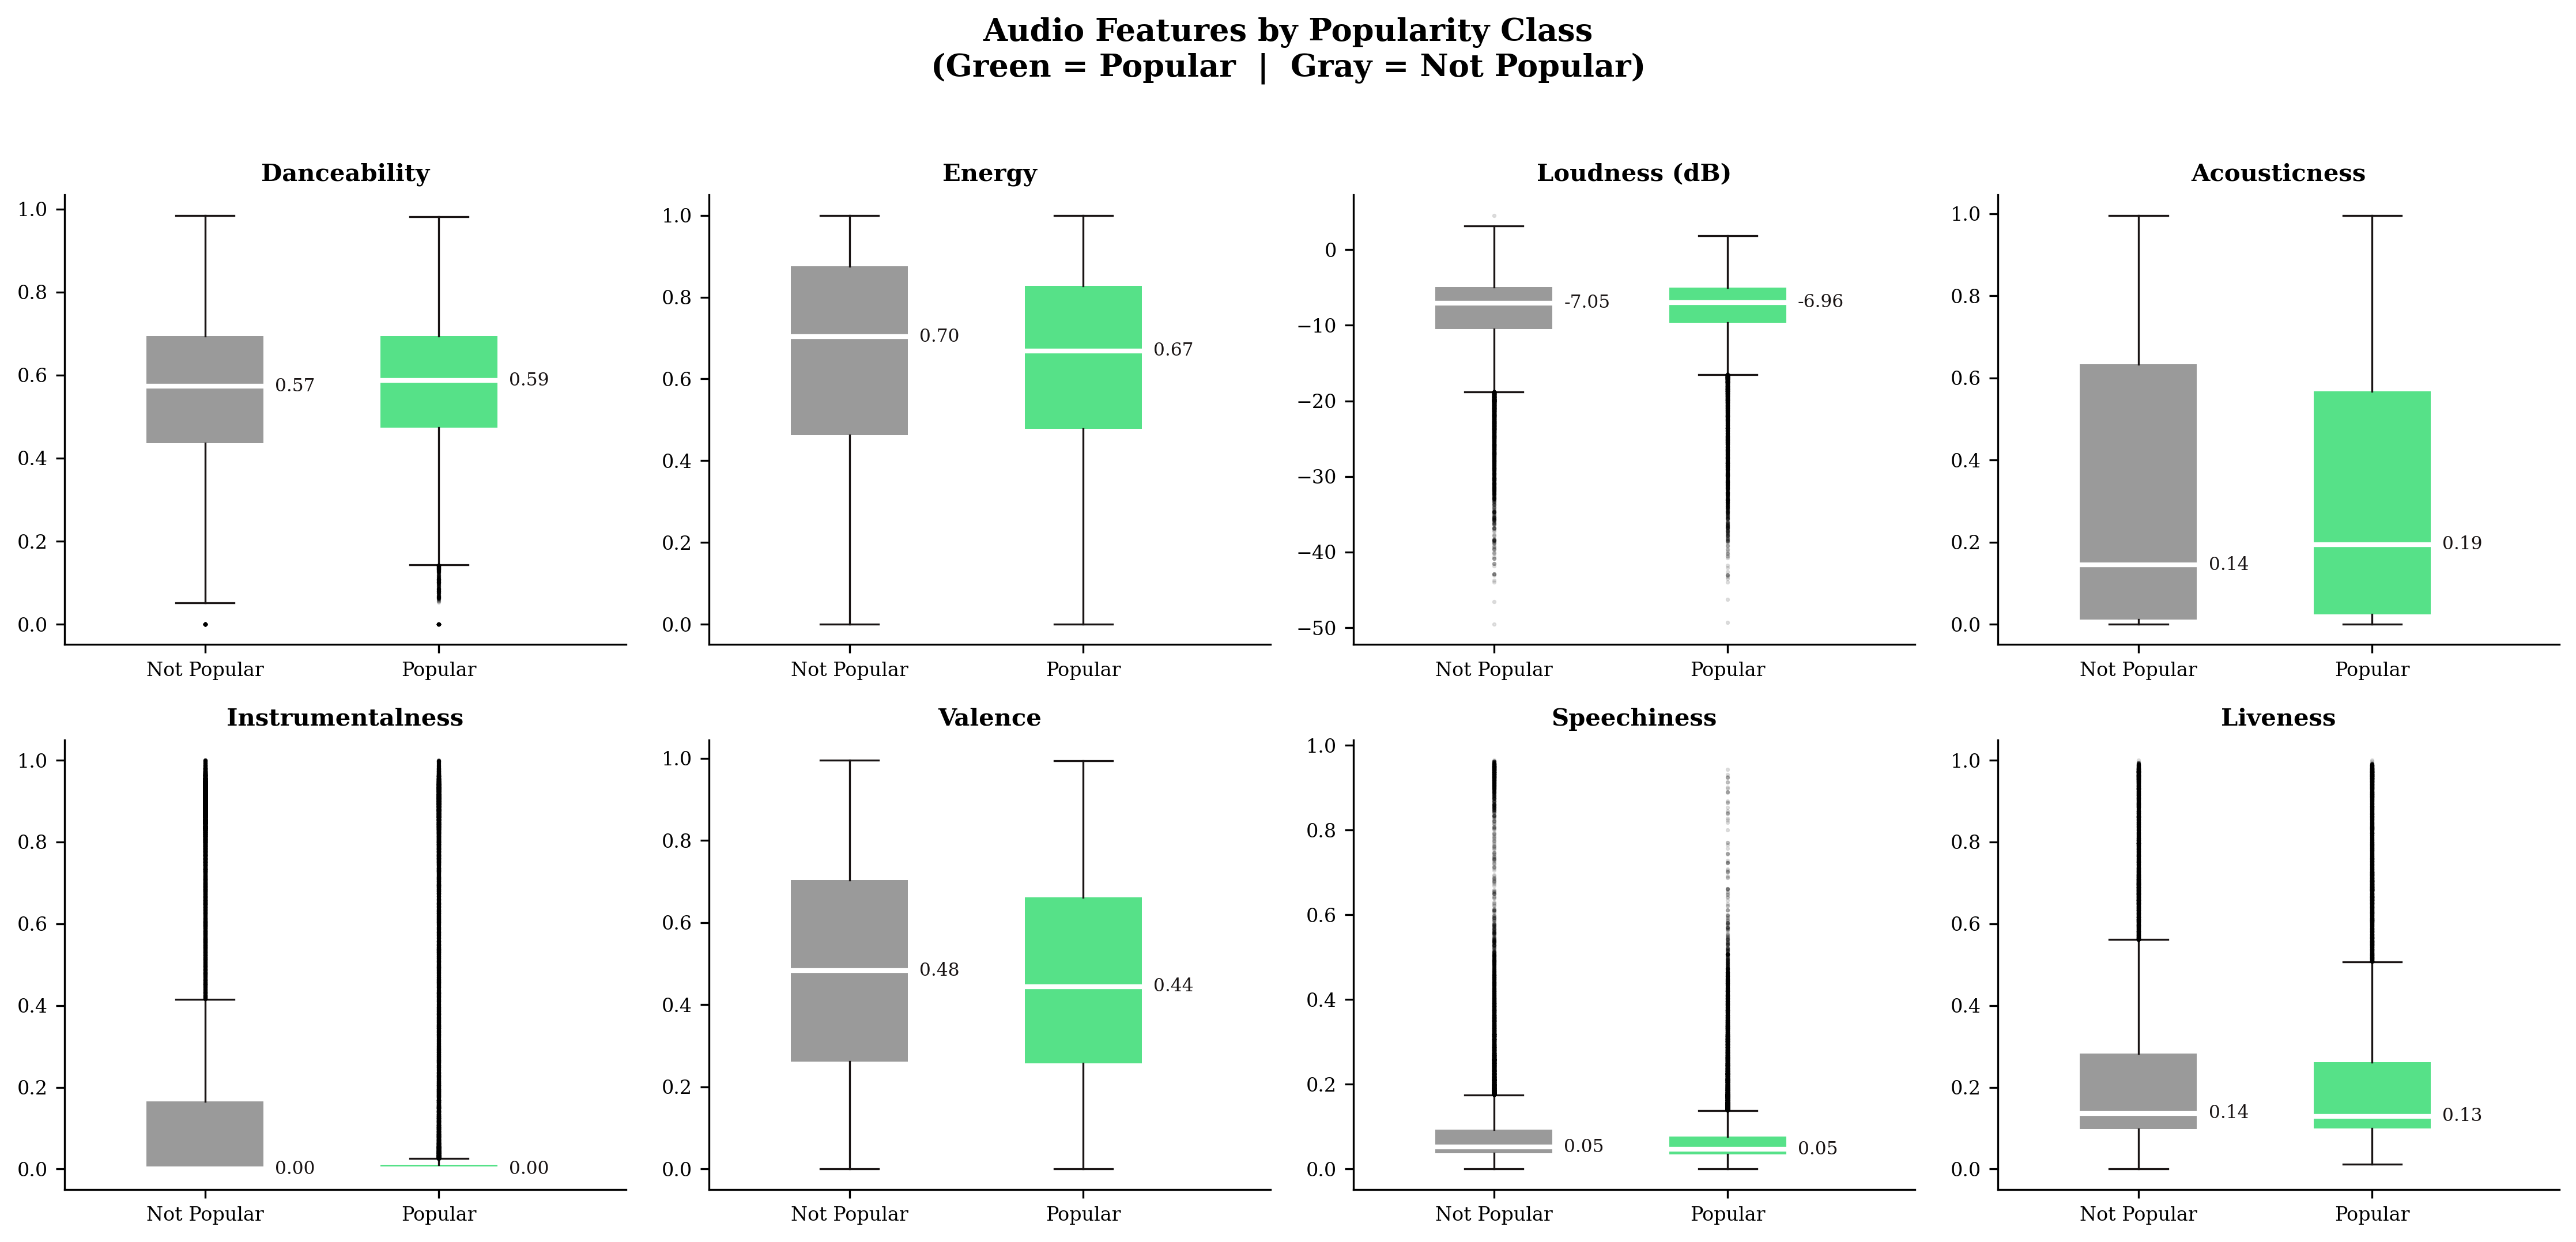
\includegraphics[width=\textwidth]{ch2_boxplots.png}
    \caption{Boxplots of audio features grouped by binary popularity class. Green = popular (score~$>$~35), gray = not popular (score~$\leq$~35). The largest visible separations appear in loudness, instrumentalness, danceability, and acousticness.}
    \label{fig:ch2_boxplots}
\end{figure}
 
\section{Correlation Structure}
 
Figure~\ref{fig:ch2_corr} shows the Pearson correlation heatmap for all 13 numeric predictors and the popularity response. The strongest pairwise correlation is between \texttt{energy} and \texttt{loudness} ($r = 0.762$), expected because louder tracks perceptually feel more energetic. \texttt{acousticness} is strongly negatively correlated with energy ($r = -0.734$) and loudness ($r = -0.590$), reflecting the acoustic--electric divide in production style. \texttt{valence} and \texttt{danceability} share a moderate positive correlation ($r = 0.477$), consistent with the intuition that upbeat songs are more danceable.
 
Correlations between any individual predictor and \texttt{popularity} are weak --- the largest in absolute value is \texttt{instrumentalness} at $r = -0.095$. This does not mean audio features are uninformative; it means the relationship is likely nonlinear and genre-conditional. The energy--loudness--acousticness cluster will be revisited as a multicollinearity concern in Chapter 4.
 
\begin{figure}[H]
    \centering
    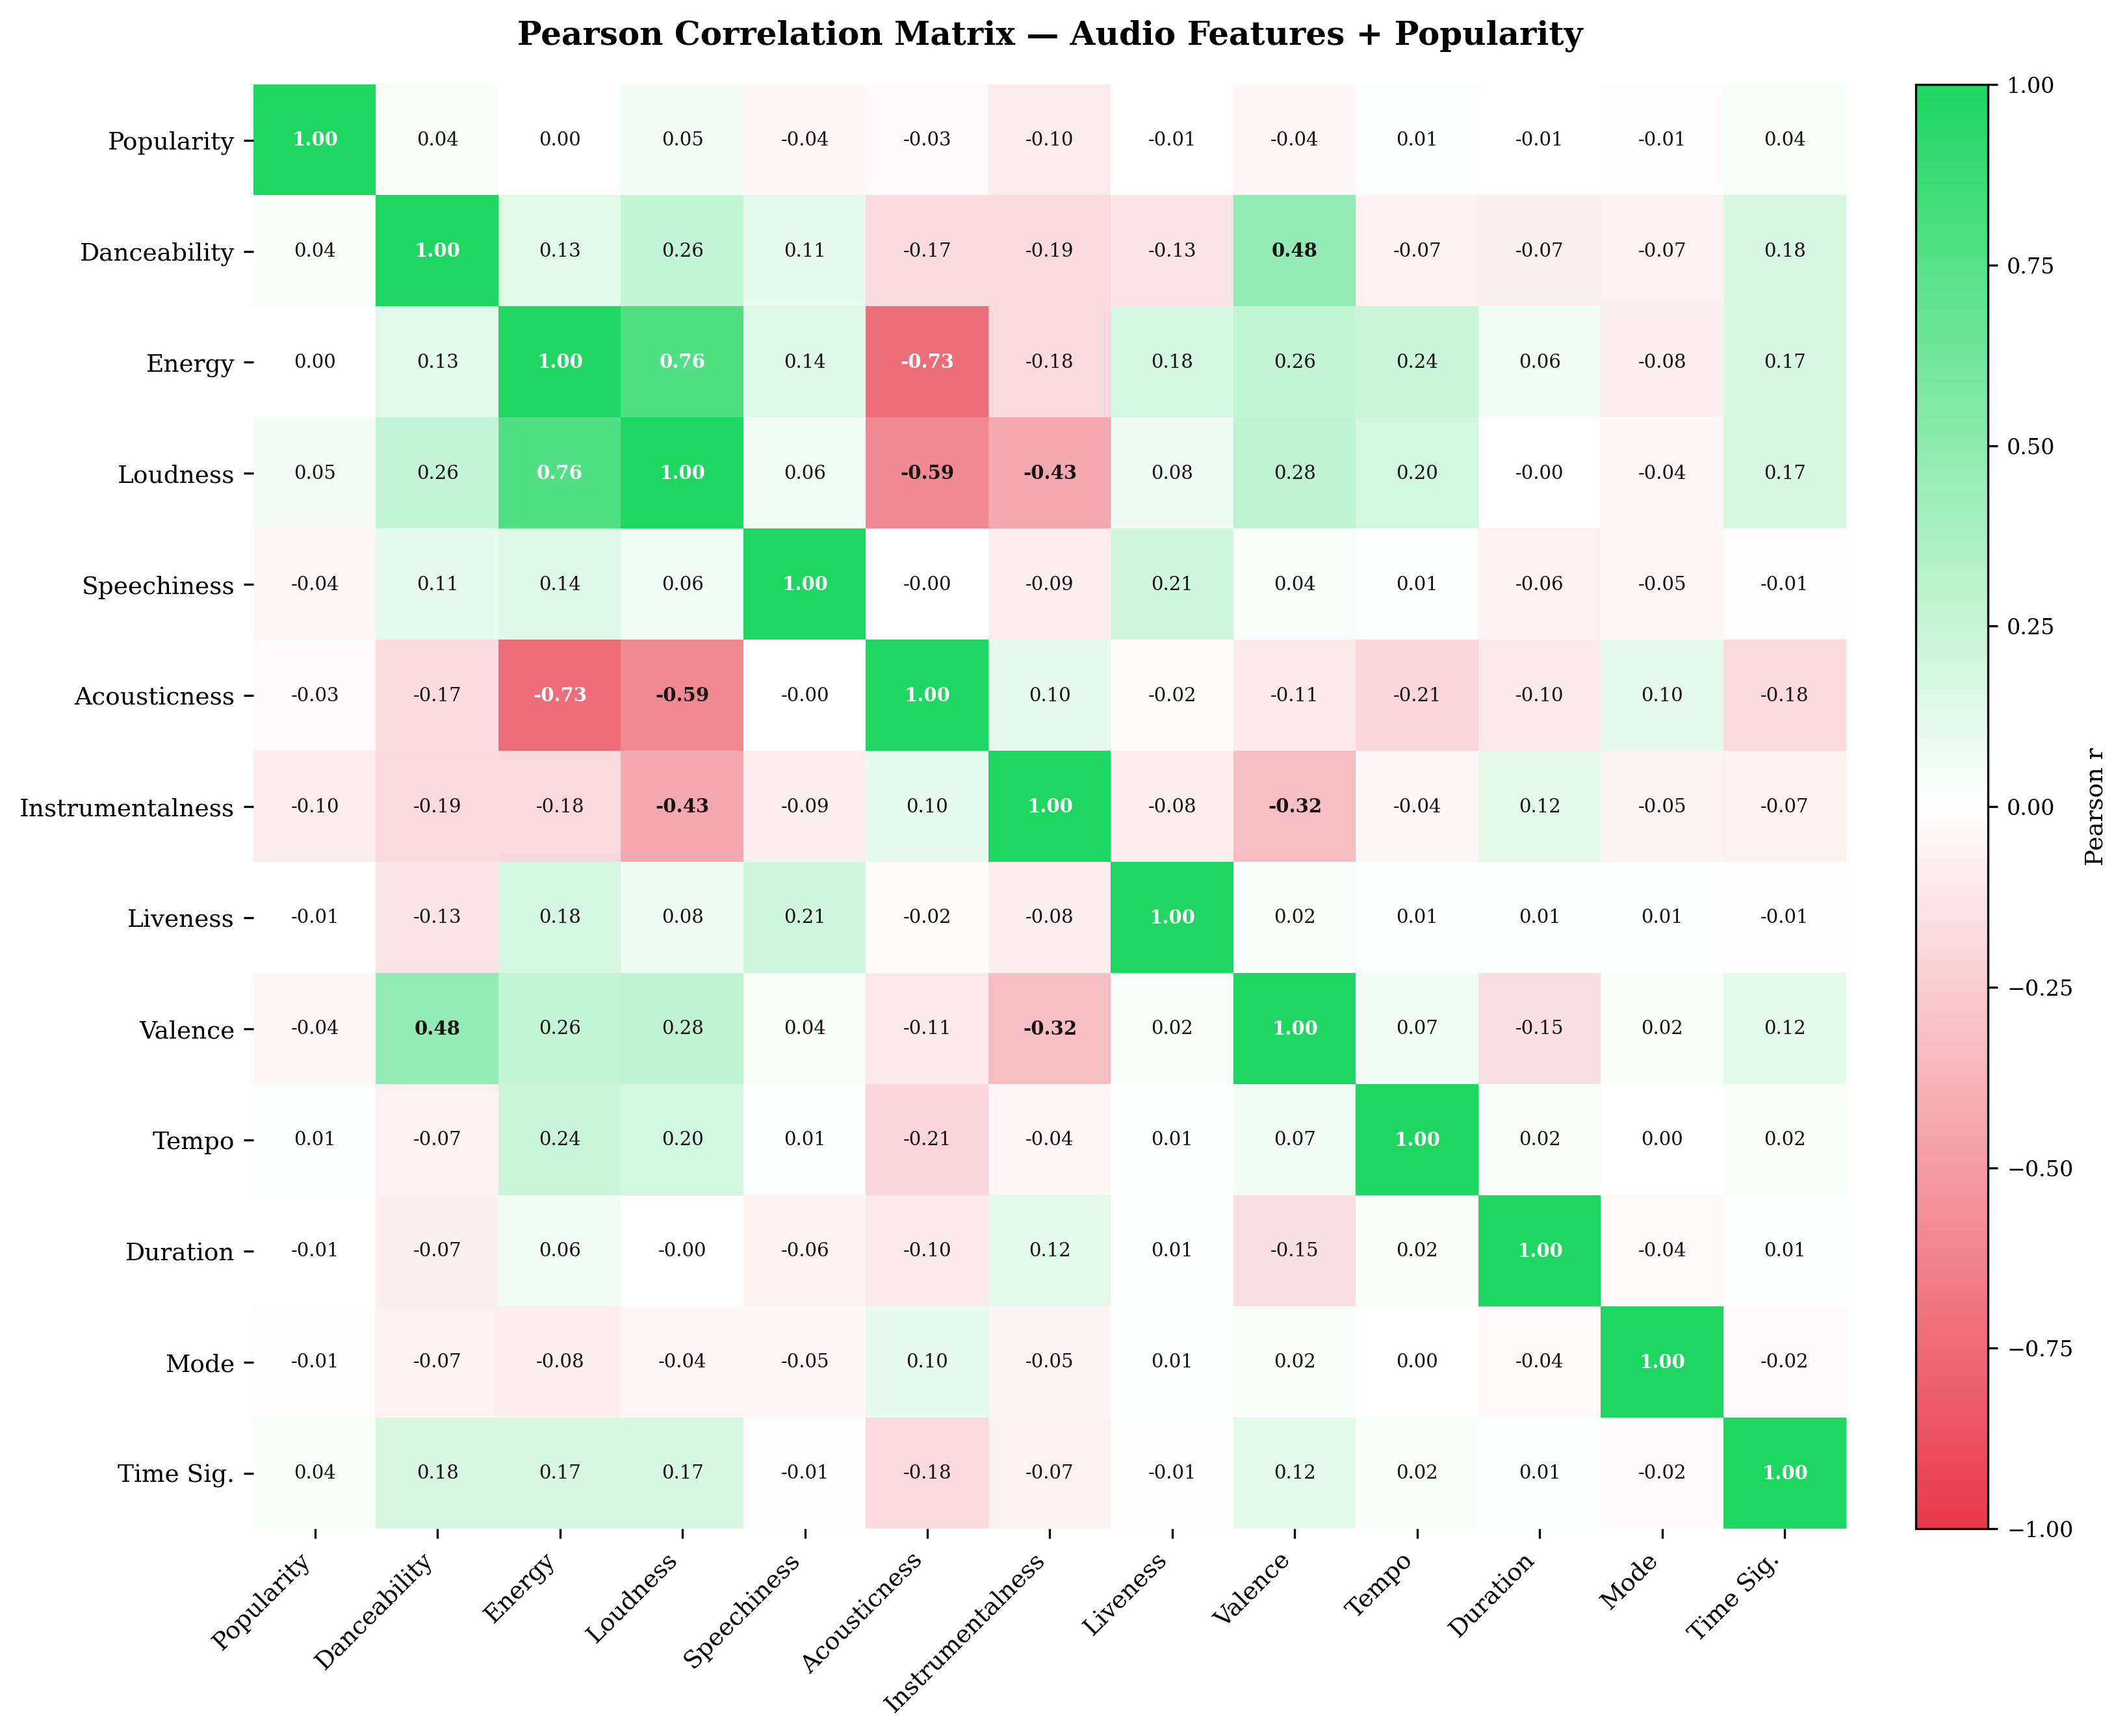
\includegraphics[width=0.82\textwidth]{ch2_corr.png}
    \caption{Pearson correlation heatmap for the 13 numeric predictors and the popularity response. Color runs from dark red ($r = -1$) through white ($r = 0$) to dark green ($r = +1$).}
    \label{fig:ch2_corr}
\end{figure}
 
\section{Missing Data and Anomalies}
 
All 14 numeric columns contain zero missing values after the three-row drop.
 
\begin{itemize}
    \item \textbf{Tempo = 0 BPM} (157 tracks): Spotify encodes estimation failure as 0. Replaced with \texttt{NaN} and imputed using the training-set median of 122.0 BPM.
    \item \textbf{Time signature = 0} (163 tracks): Same estimation failure code. Replaced with \texttt{NaN} and imputed using the training-set mode of 4.
    \item \textbf{Extreme durations}: 16 tracks under 30 seconds (interludes or sound effects) and 603 tracks over 10 minutes. Retained; log transformation of \texttt{duration\_ms} reduces leverage.
    \item \textbf{Popularity = 0} (16{,}019 tracks, 14.1\%): Legitimate entries for obscure tracks. Retained as-is; they anchor the lower end of both the continuous and binary response.
\end{itemize}
 
% ============================================================
%  CHAPTER 3 — Simple Linear Regression
% ============================================================
\chapter{Simple Linear Regression}
 
\section{The Question}
 
Does a track's loudness, taken alone, predict its Spotify popularity score? Loudness is the audio feature that most directly reflects production decisions. Mixing and mastering actively push it to the limits of what streaming normalization allows. If loudness drives popularity, that is an actionable finding for artists.
 
\section{Method in Brief}
 
Simple linear regression fits a straight line to the data by minimizing the sum of squared vertical distances between each observed value and the line. The result is a slope, which tells us how much the response changes for a one-unit increase in the predictor, and an intercept, which gives the predicted response when the predictor equals zero.

\section{Why This Method?}
 
Both the response (popularity, 0-100) and the predictor (loudness, measured in dB) are continuous. SLR is the right starting point, because it is fully interpretable, requires no tuning, and produces a coefficient that directly quantifies the loudness and popularity relationship. A more flexible model would answer a different question. The goal here is to isolate a single variable and understand it cleanly before introducing additional complexity.
 
\section{Data Setup}
 
\begin{itemize}
    \item \textbf{Response}: \texttt{popularity} (continuous, 0--100).
    \item \textbf{Predictor}: \texttt{loudness} (dB, range $-49.5$ to $+4.5$). No transformation needed, because loudness is already on a linear scale.
    \item \textbf{Split}: The model is fit on the 79{,}799-row training set; all diagnostics use training residuals; final performance is reported on the held-out 17{,}100-row test set.
\end{itemize}
 
Among the 13 available audio features, loudness is chosen as the SLR predictor because it has the highest marginal $R^2$ with popularity among the features ($R^2 = 0.0025$), slightly ahead of instrumentalness ($R^2 = 0.0091$ but in the negative direction). the marginal $R^2$ bar chart (Figure~\ref{fig:ch3_r2_compare}) shows the marginal $R^2$ for all 13 predictors, confirming that no single feature explains more than 1\% of the variance in popularity.
 
 
\section{Analysis}
 
The fitted model on the training set is:
 
\begin{equation}
\widehat{\texttt{popularity}} = 35.086 + 0.224 \times \texttt{loudness}
\label{eq:slr}
\end{equation}
 
Since loudness is measured in dB and ranges from approximately $-50$ to $0$, the intercept of 35.09 corresponds to the predicted popularity at 0 dB, the loudest possible value. The slope of 0.224 means that each 1 dB increase in loudness is associated with a 0.224 increase in popularity points. Equivalently, a track that is 10 dB louder than another is predicted to score about 2.2 popularity points higher, all else equal.
 
Table~\ref{tab:ch3_results} summarizes the full regression output.
 
\begin{table}[H]
\centering
\caption{Simple linear regression results: popularity regressed on loudness. Fit on training set ($n = 79{,}799$). SE = standard error; CI = 95\% confidence interval.}
\label{tab:ch3_results}
\begin{tabular}{lrrrrl}
\toprule
\textbf{Term} & \textbf{Estimate} & \textbf{SE} & \textbf{$t$-stat} & \textbf{$p$-value} & \textbf{95\% CI} \\
\midrule
Intercept (loudness = 0) & 35.086 & 0.148 & 237.1 & $< 0.001$ & [34.796,\ 35.376] \\
Loudness (dB)            &  0.224 & 0.013 &  17.0 & $< 0.001$ & [0.198,\ 0.249] \\
\midrule
\multicolumn{6}{l}{$R^2 = 0.0024$ \quad RMSE (train) $= 22.24$ \quad RMSE (test) $= 22.32$ \quad $F(1,79797) = 290.5$, $p < 0.001$} \\
\bottomrule
\end{tabular}
\end{table}
 
Figure~\ref{fig:ch3_scatter} shows the scatter plot of loudness versus popularity with the fitted regression line, along with prediction intervals. The line is clearly positive but the scatter is enormous relative to the slope.
 
\begin{figure}[H]
    \centering
    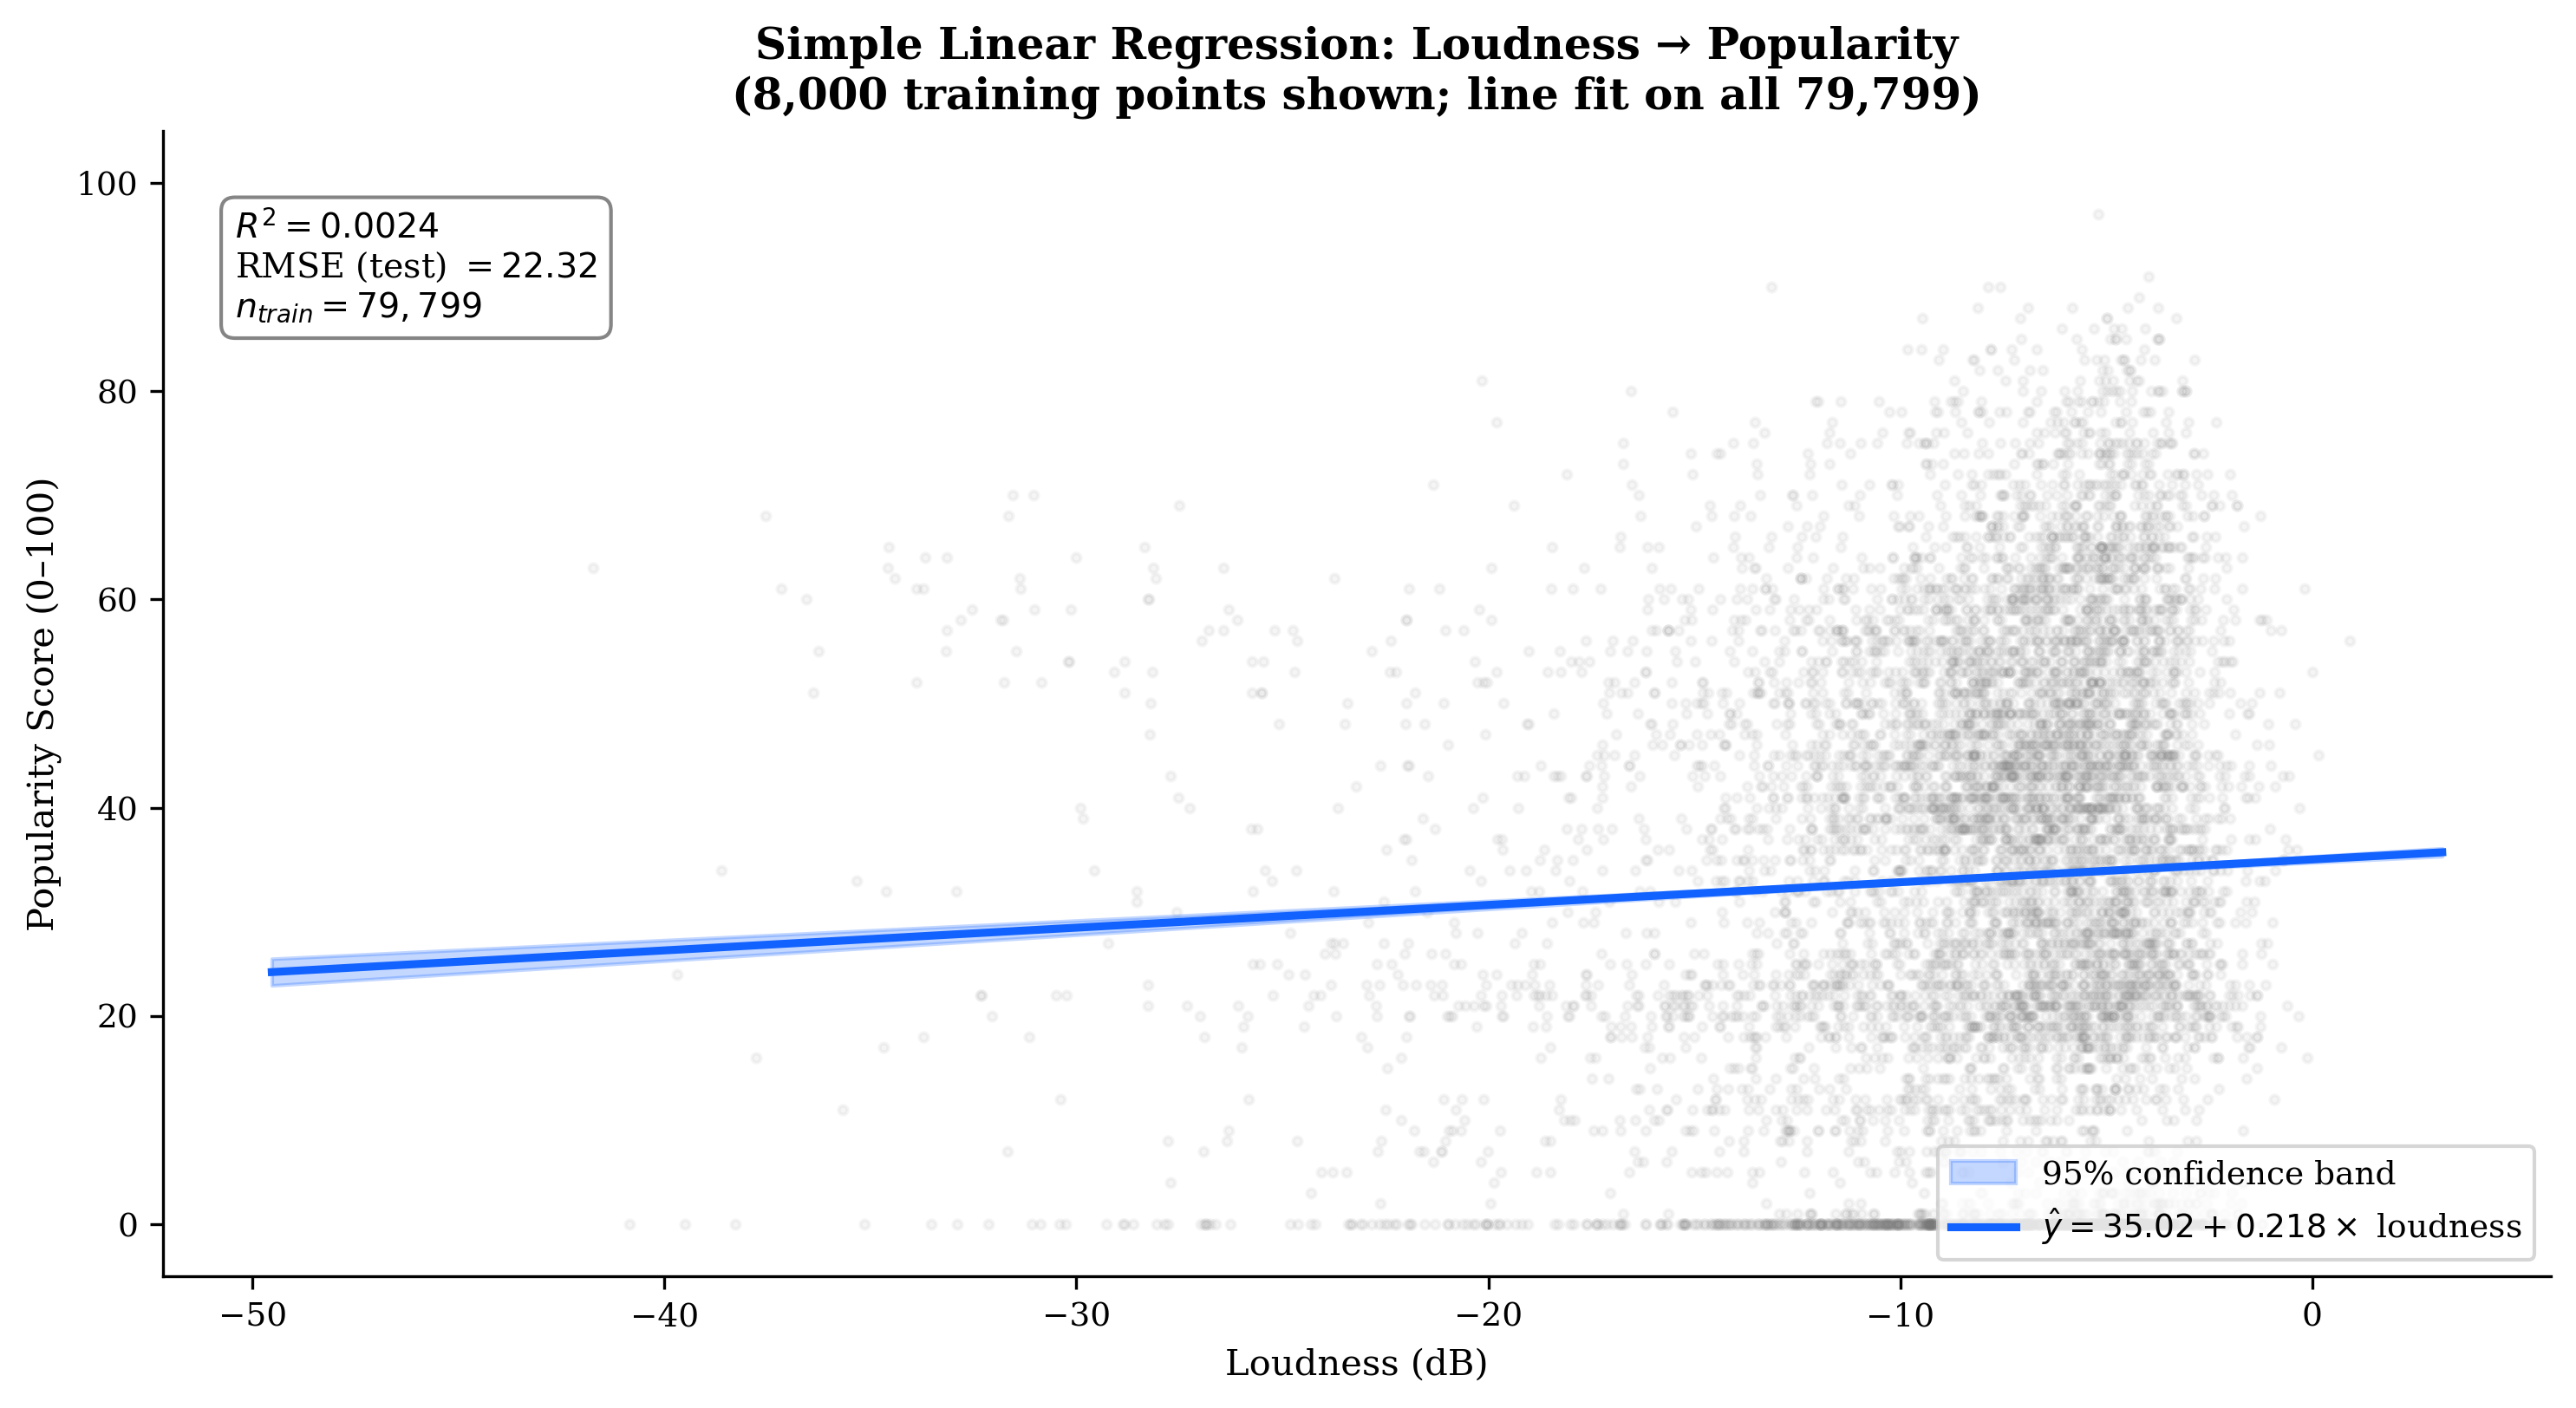
\includegraphics[width=\textwidth]{ch3_scatter.png}
    \caption{Scatter plot of loudness (dB) vs.\ popularity with the fitted SLR line (blue) and 95\% confidence band (shaded). Points are sampled (n = 8{,}000) for visual clarity.}
    \label{fig:ch3_scatter}
\end{figure}
 
\section{Diagnostics and Tuning}

\textbf{Linearity.} The LOWESS curve overlaid on the scatter plot in Figure~\ref{fig:ch3_scatter} is approximately linear across the bulk of the loudness range, with some curvature at the extreme quiet end, where very few observations exist.
 
\textbf{Residual diagnostics.} Figure~\ref{fig:ch3_diagnostics} shows the four standard residual plots. The residuals vs.\ fitted values plot reveals a fan-shaped pattern: variance is somewhat lower at the extreme low and extreme high fitted values and larger in the middle range. This mild heteroscedasticity is expected given that popularity is bounded between 0 and 100 --- the model cannot predict negative or above-100 values, which compresses variance at the extremes. The Q--Q plot shows light-tailed, near-normal residuals (skewness $= 0.036$, kurtosis $= -0.926$), consistent with the large sample size, which approximately meets the normality assumption. The scale--location plot confirms the mild heteroscedasticity but shows no dramatic trend.
 
\begin{figure}[H]
    \centering
    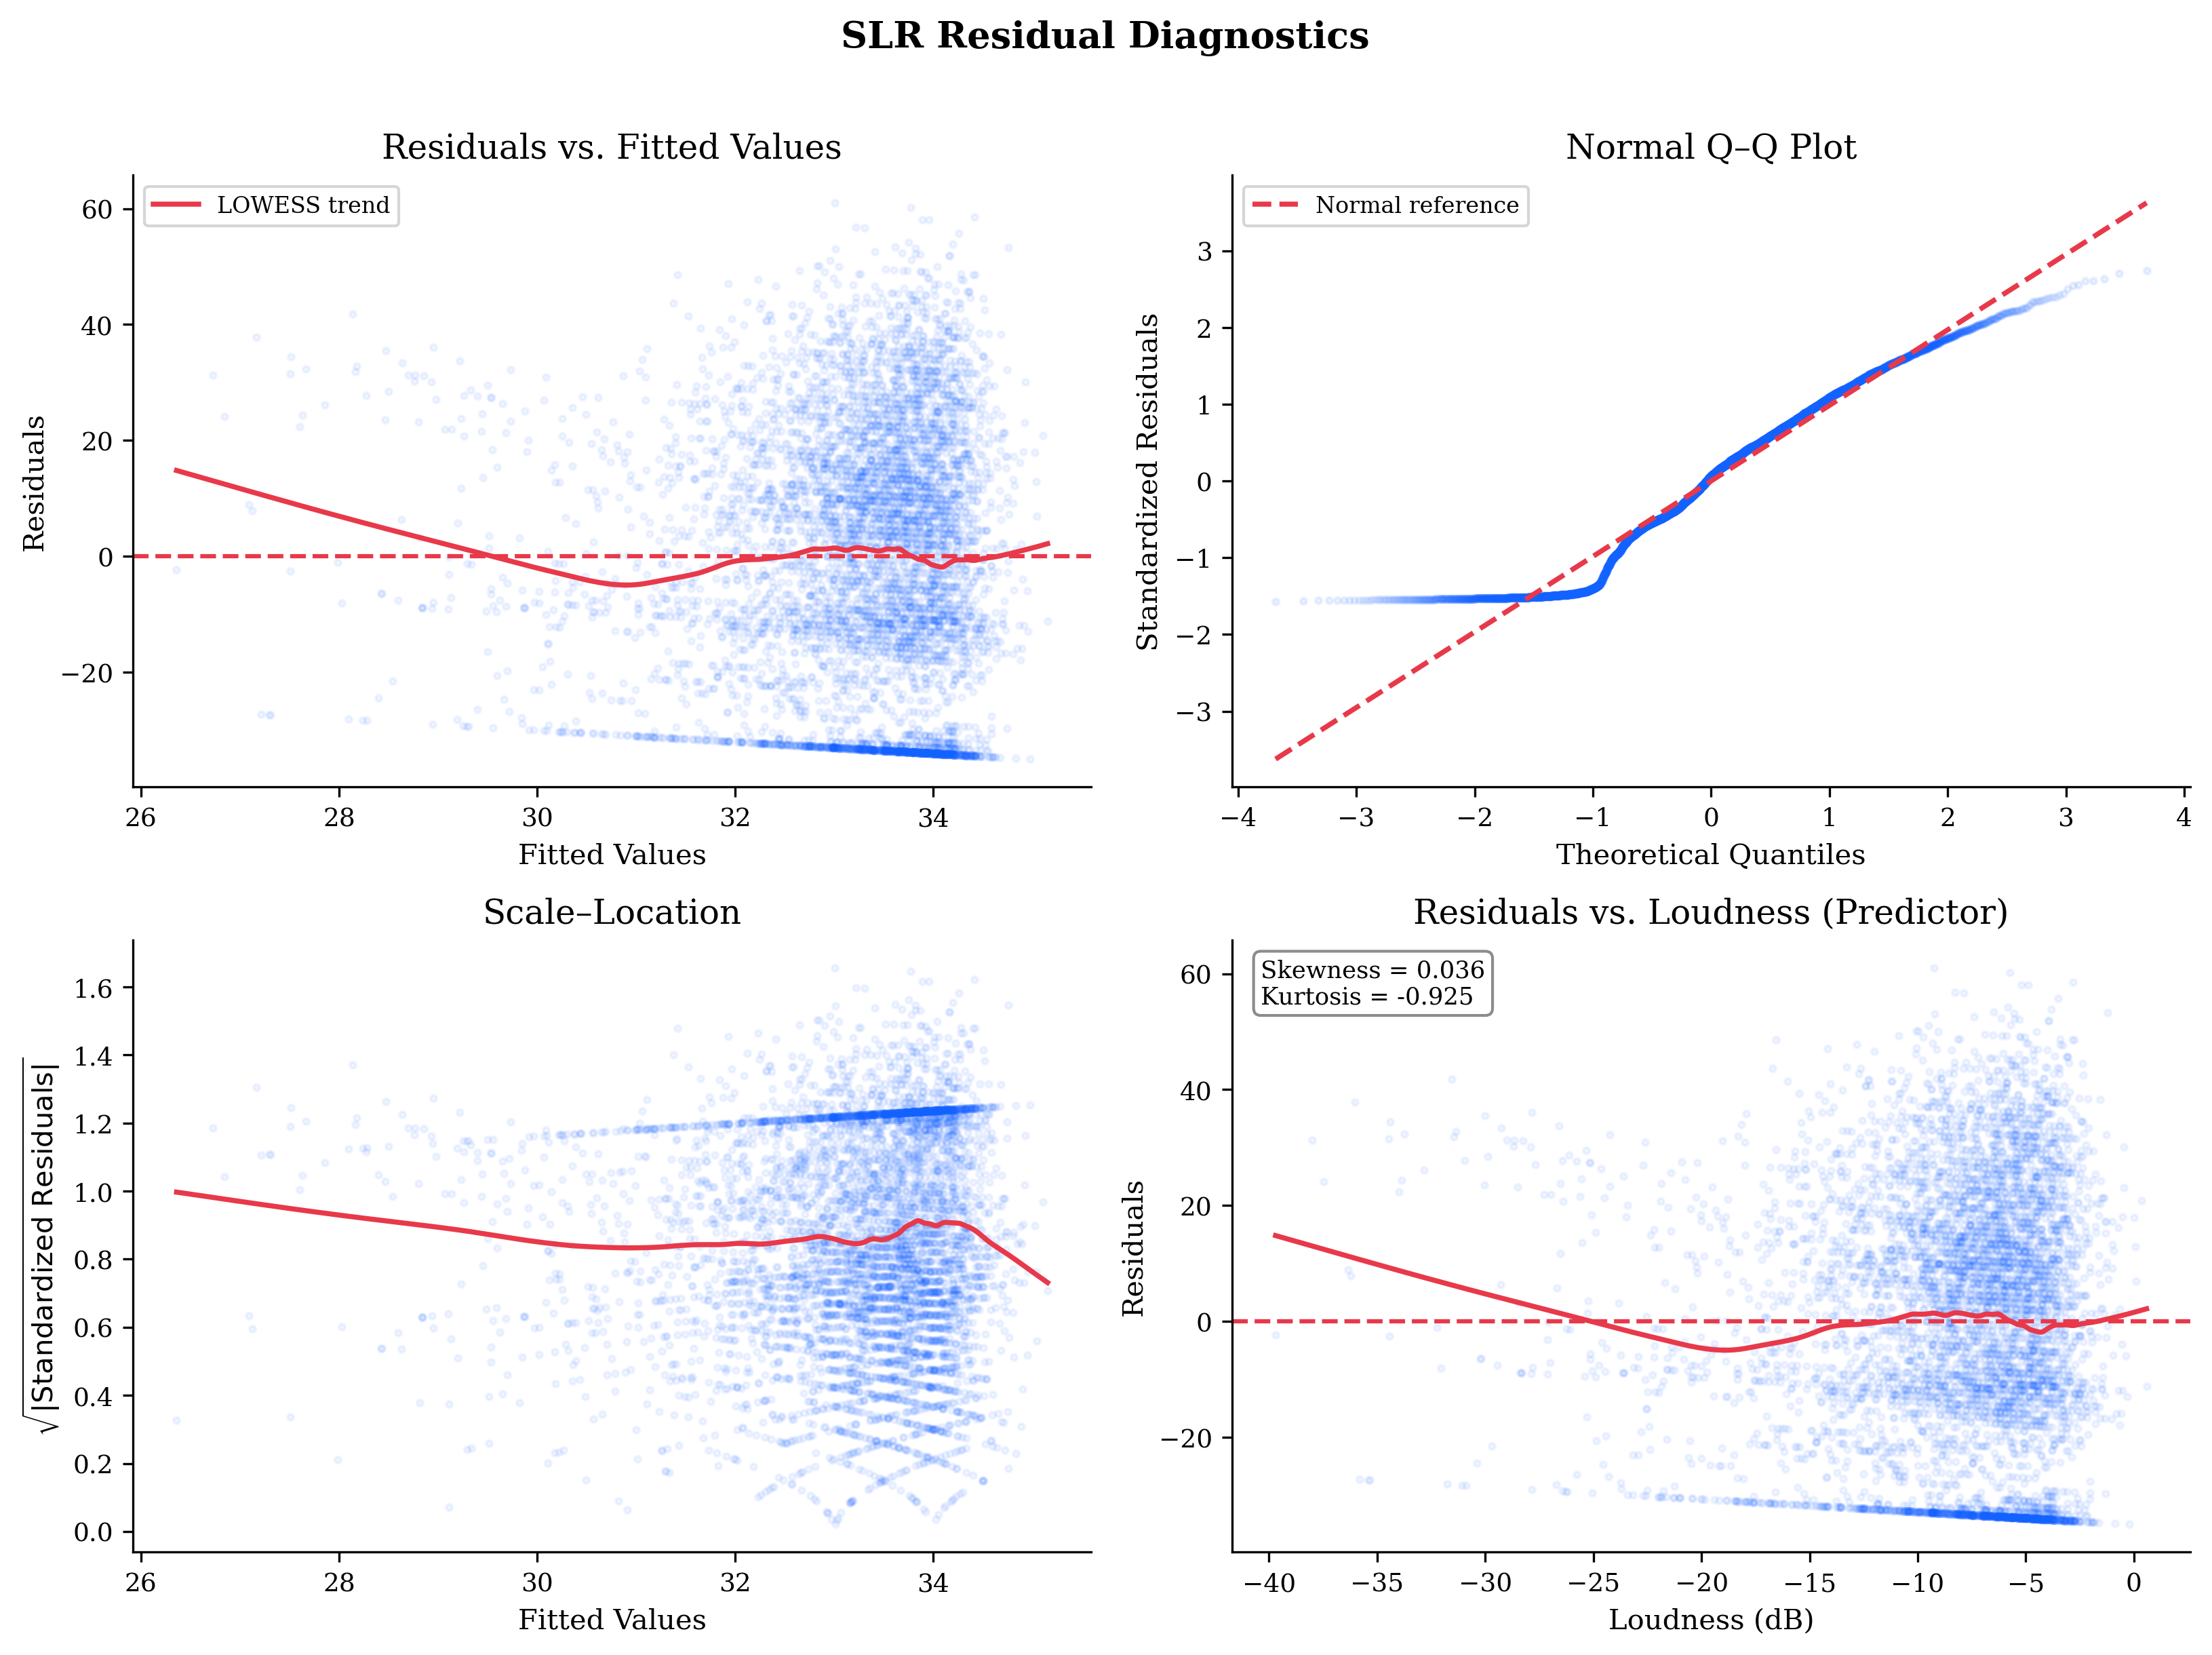
\includegraphics[width=\textwidth]{ch3_diagnostics.png}
    \caption{Standard SLR diagnostic plots. Top-left: residuals vs.\ fitted values (mild heteroscedasticity visible but no systematic pattern).}
    \label{fig:ch3_diagnostics}
\end{figure}
 
\textbf{Independence.} Within a genre the tracks are not time-series data, so serial autocorrelation is not a concern. The multi-genre duplication introduces mild dependence for repeated tracks, but because loudness is identical across a track's repeated rows, this does not bias the slope estimate.
 
\textbf{Test set generalization.} The training RMSE (22.24) and test RMSE (22.32) are essentially identical, confirming no overfitting. This is expected for a model with a single predictor fit on 79{,}000 observations.
 
\section{Findings}
 
The $p$-value on the slope is effectively zero, meaning the positive loudness--popularity relationship is real and not a sampling artifact. However, $R^2 = 0.0024$. Loudness alone explains 0.24\% of the variance in popularity. The test RMSE of 22.32 on a 0--100 scale indicates that a typical prediction is off by more than 22 popularity points. The model is statistically detectable but practically ineffective as a standalone predictor.
 
Figure~\ref{fig:ch3_r2_compare} provides a visual comparison of $R^2$ values across all 13 single-predictor models. None exceeds 1\%, and most are near zero, making clear that popularity cannot be explained by any individual audio feature.
 
\begin{figure}[H]
    \centering
    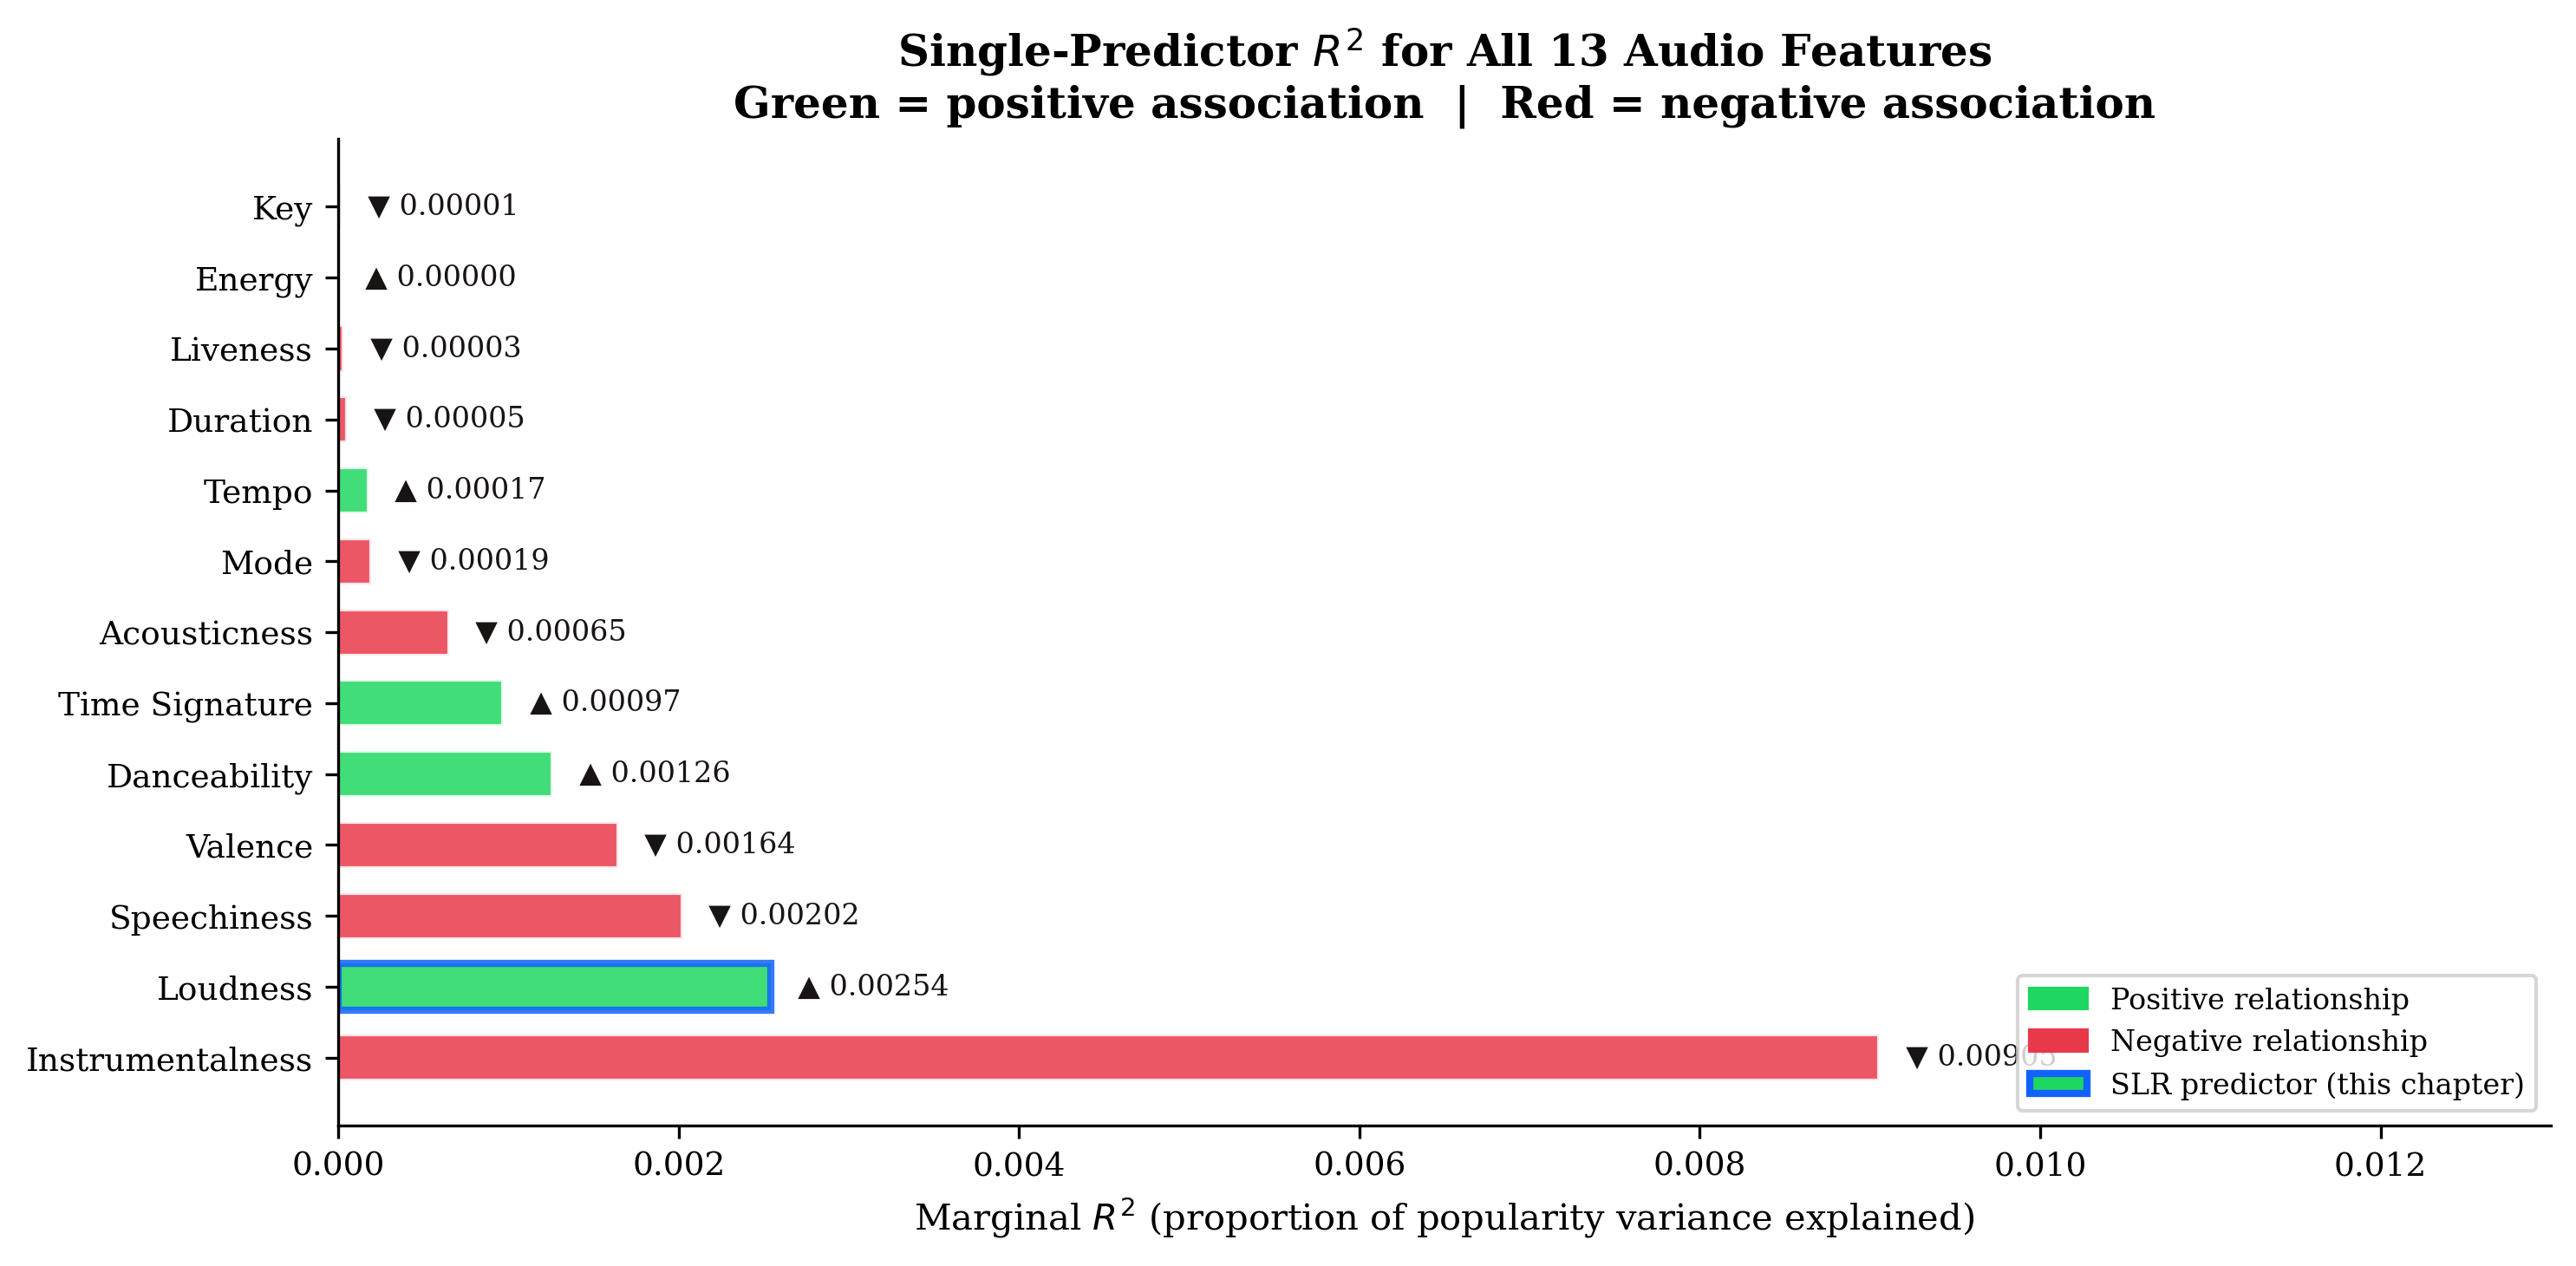
\includegraphics[width=0.85\textwidth]{ch3_r2_compare.png}
    \caption{Marginal $R^2$ for each audio feature regressed individually on popularity. The tallest bar (instrumentalness) reaches only 0.9\%.}
    \label{fig:ch3_r2_compare}
\end{figure}
 
\chapter{Multiple Linear Regression}
 
\section{The Question}
 
Which combination of audio features, musical key, time signature, and genre best predicts a track's popularity score when modeled jointly? Chapter 3 established that loudness alone explains only 0.24\% of the variance in popularity.
 
\section{Method in Brief}
 
Multiple linear regression extends the single-predictor model by fitting a hyperplane to the data rather than a line. Each predictor has its own coefficient, which represents the expected change in the response to a one-unit increase in that predictor, holding all other predictors constant. The model is still fit by minimizing the sum of squared residuals, and the resulting weights are fully interpretable as weighted combinations of the input features.
 
\section{Why This Method?}
 
The goal is to quantify how much variance all audio features collectively explain, and to obtain coefficient estimates that isolate the partial effect of each feature net of the others. Multiple regression is the canonical tool for both. It also serves as the explicit baseline for regularization methods.
 
\section{Data Setup}
 
\textbf{Response}: \texttt{popularity} (continuous, 0-100).
 
\textbf{Predictors}: The full design matrix contains 139 columns organized as follows.
 
\begin{itemize}
    \item \textbf{10 continuous audio features}: danceability, energy, loudness, speechiness, acousticness, instrumentalness, liveness, valence, tempo, and log(duration\_ms). Duration is log-transformed to reduce the influence of extreme values (skewness reduced from 11.2 to near-zero).
    \item \textbf{2 binary features}: mode (major = 1, minor = 0) and explicit (1/0).
    \item \textbf{11 key dummy variables}: one-hot encoding of musical key (0--11), with key = 0 (C major) as the reference category.
    \item \textbf{3 time-signature dummy variables}: one-hot encoding of time signature, with value = 1 as the reference.
    \item \textbf{113 genre dummy variables}: one-hot encoding of \texttt{track\_genre} (114 levels), with \textit{acoustic} as the reference genre.
\end{itemize}
 
All continuous predictors are standardized to zero mean and unit variance using training-set parameters before fitting, so coefficients are on a comparable scale. Sentinel values (tempo = 0, time signature = 0) are imputed with training-set median and mode respectively, as described in Chapter 2.
 
\textbf{Split}: 70/15/15 stratified split as all other chapters ($n_{\text{train}} = 79{,}799$).
 
\section{Analysis}
 
\subsection{Dummy Variables}
 
Genre is a nominal categorical variable with 114 levels. To include it in a linear model, it must be converted into a set of binary indicator columns—one per genre level, with one reference category. This produces 113 dummy variables of the form $\mathbf{1}$ for each non-reference genre $k$.
 
The musical key is treated as nominal rather than ordinal. There is no reason to assume that key 11 is ``11 times'' anything relative to key 0. It is therefore also one-hot encoded into 11 dummy variables. The two binary variables, mode and explicit, are already coded as 0/1.
 
the genre coefficient figure in Appendix~C shows the ten genres with the largest positive and ten with the largest negative coefficients in the fitted model, holding all audio features constant.
 
 
\subsection{Multicollinearity and VIF}
 
Before interpreting individual coefficients, the degree of multicollinearity among predictors must be assessed. The Variance Inflation Factor measures how much the variance of a coefficient estimate is inflated due to correlation with other predictors. A VIF above 10 indicates serious multicollinearity; values between 5 and 10 warrant caution; values below 5 are generally acceptable.
 
VIF was computed for the 12 continuous and binary predictors. Table~\ref{tab:ch4_vif} reports the results.
 
\begin{table}[H]
\centering
\caption{Variance Inflation Factors for the 12 continuous and binary predictors. All values are below 5, indicating acceptable multicollinearity. The energy--loudness--acousticness cluster produces the highest VIFs.}
\label{tab:ch4_vif}
\begin{tabular}{lr}
\toprule
\textbf{Predictor} & \textbf{VIF} \\
\midrule
Energy           & 4.229 \\
Loudness         & 3.270 \\
Acousticness     & 2.426 \\
Valence          & 1.601 \\
Danceability     & 1.520 \\
Instrumentalness & 1.456 \\
Speechiness      & 1.238 \\
Liveness         & 1.142 \\
Explicit         & 1.142 \\
Tempo            & 1.086 \\
Log Duration     & 1.082 \\
Mode             & 1.025 \\
\bottomrule
\end{tabular}
\end{table}
 
The highest VIF is energy at 4.229, reflecting its strong correlations with loudness ($r = 0.762$) and acousticness ($r = -0.734$). However, no VIF exceeds 5, meaning that while some redundancy exists among the audio features, it is not severe enough to destabilize the coefficient estimates. All predictors are retained.
 
\subsection{Subset Selection}
 
With 139 predictors, exhaustive best-subset selection is computationally infeasible. Forward stepwise selection was applied to the 12 continuous and binary predictors (excluding dummy variables) to determine the order in which features enter the model and to compute AIC and BIC at each step. Table~\ref{tab:ch4_subset} reports the results.
 
\begin{table}[H]
\centering
\caption{Forward stepwise selection path (selected steps shown). AIC decreases at every step; the full 12-predictor model achieves the lowest AIC (719{,}802). All values to three decimal places.}
\label{tab:ch4_subset}
\small
\begin{tabular}{rlr}
\toprule
\textbf{Step} & \textbf{Feature Added} & \textbf{AIC} \\
\midrule
1  & Instrumentalness & 721{,}023.680 \\
3  & Danceability     & 720{,}348.840 \\
5  & Explicit         & 719{,}906.260 \\
8  & Mode             & 719{,}823.180 \\
11 & Loudness         & 719{,}803.370 \\
12 & Acousticness     & 719{,}802.720 \\
\midrule
\multicolumn{3}{l}{Full model BIC: 719{,}923.460 \quad $R^2$: 0.024 \quad Adj.\ $R^2$: 0.024} \\
\bottomrule
\end{tabular}
\end{table}
 
Two observations stand out. First, AIC continues to decrease all the way to step 12, meaning no feature is redundant enough to be dropped when the others are present, the full model is the best model on this predictor set. Second, the AIC improvement is steep at steps 1--5 and flattens sharply after step 6. This suggests that roughly five features carry the bulk of the signal and the remaining features contribute only marginally, a pattern that foreshadows the lasso results in Chapter 7.
 
\section{Diagnostics and Tuning}
 
\textbf{Cross-validation.} Five-fold cross-validation on the training set yields a mean RMSE of $19.184 \pm 0.135$, very close to the test RMSE of 19.248. The negligible gap confirms that the model generalizes without overfitting, as the training set is sufficiently large that the effective degrees of freedom per observation remain favorable.
 
\textbf{Residual plots.} Figure~\ref{fig:ch4_diagnostics} shows the standard residual diagnostic plots for the full model. The residuals vs.\ fitted values plot shows the same bounded-response heteroscedasticity, with variance narrowing at the extremes because predicted popularity cannot exceed 0 or 100. The Q--Q plot is near-normal in the central range with slightly heavier tails. No systematic curvature is present, consistent with the model's linearity assumption being approximately met.
 
\begin{figure}[H]
    \centering
    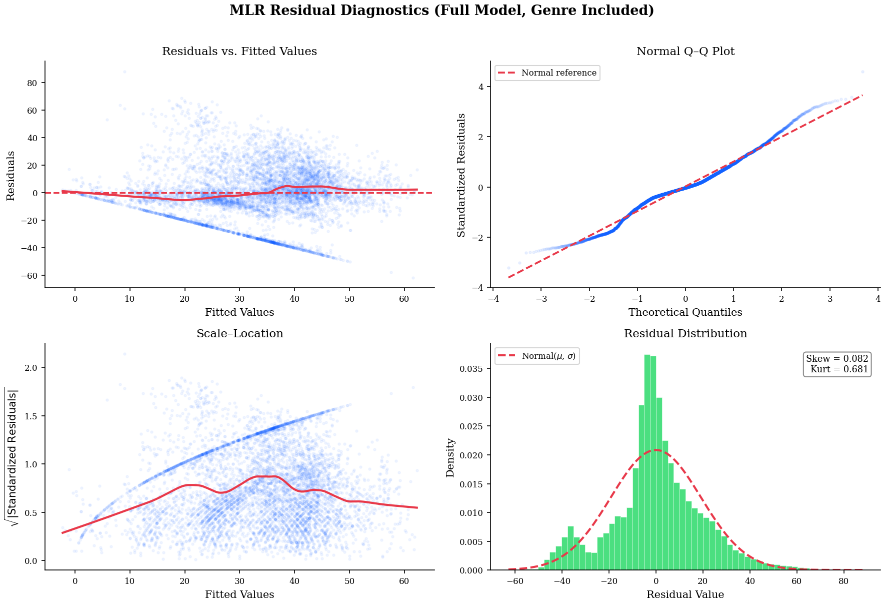
\includegraphics[width=\textwidth]{ch4_diagnostics.png}
    \caption{Residual diagnostic plots for the full MLR model. Top-left: residuals vs.\ fitted values with LOWESS smoother. Top-right: Normal Q--Q plot. Bottom-left: scale--location plot. Bottom-right: histogram of residuals with normal overlay.}
    \label{fig:ch4_diagnostics}
\end{figure}
 
\section{Findings}
 
Table~\ref{tab:ch4_model_comparison} compares all three MLR specifications against the Chapter 3 SLR baseline.
 
\begin{table}[H]
\centering
\caption{Model performance comparison: SLR baseline, MLR without genre, and MLR with genre dummies. Test metrics are evaluated on the locked 17{,}100-row test set.}
\label{tab:ch4_model_comparison}
\begin{tabular}{lrrr}
\toprule
\textbf{Model} & \textbf{Train $R^2$} & \textbf{Test $R^2$} & \textbf{Test RMSE} \\
\midrule
SLR --- loudness only (Ch.\ 3)  & 0.002 & 0.003 & 22.320 \\
MLR --- audio features only     & 0.027 & 0.023 & 22.094 \\
MLR --- audio features + genre  & 0.261 & 0.259 & 19.248 \\
\bottomrule
\end{tabular}
\end{table}
 
The jump from 2.7\% to 26.1\% explained variance when genre dummies are added. Audio features alone are nearly as weak as the single-predictor model, adding 11 features to loudness only improves RMSE from 22.32 to 22.09. Genre membership, by contrast, reduces RMSE by 3 full points (22.09 $\to$ 19.25) and explains ten times more variance.
 
Among the non-genre coefficients in the full model (Table~\ref{tab:ch4_coefs}), valence and energy  have the largest absolute values, meaning more positive-sounding and more energetic tracks are actually associated with \textit{lower} popularity in this joint model --- the opposite sign from what naive intuition might suggest. This sign reversal compared to the SLR results is a classic symptom of \textit{multicollinearity and omitted-variable confounding}: once genre is controlled for, the within-genre relationship between energy/valence and popularity can flip.
 
\begin{table}[H]
\centering
\caption{Top 10 non-genre coefficients in the full MLR model, ranked by absolute value. Predictors are standardized, so coefficients are on a comparable scale. All values reported to three decimal places.}
\label{tab:ch4_coefs}
\begin{tabular}{lrrr}
\toprule
\textbf{Predictor} & \textbf{Coefficient} & \textbf{VIF} & \textbf{Direction} \\
\midrule
Valence          & $-$1.153 & 1.601 & Negative \\
Energy           & $-$1.070 & 4.229 & Negative \\
Danceability     & $+$0.869 & 1.520 & Positive \\
Explicit         & $+$0.773 & 1.142 & Positive \\
Loudness         & $+$0.569 & 3.270 & Positive \\
Mode             & $-$0.480 & 1.025 & Negative \\
Acousticness     & $-$0.442 & 2.426 & Negative \\
Speechiness      & $-$0.373 & 1.238 & Negative \\
Key = 2 (D)      & $+$0.362 & --- & Positive \\
Log Duration     & $+$0.340 & 1.082 & Positive \\
\bottomrule
\end{tabular}
\end{table}
 
Figure~\ref{fig:ch4_coef_plot} shows the coefficient plot for all non-genre predictors, and The genre coefficient figure in Appendix~C shows all 113 genre effects.
 
\begin{figure}[H]
    \centering
    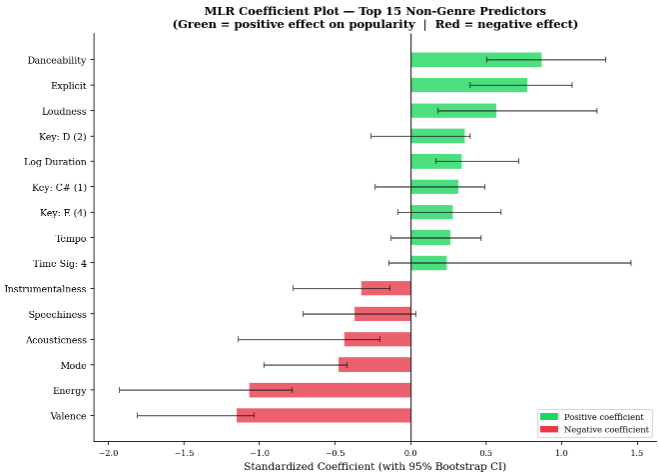
\includegraphics[width=0.88\textwidth]{ch4_coef_plot.png}
    \caption{Coefficient plot for the 15 largest non-genre predictors in the full MLR model. Error bars show 95\% confidence intervals estimated via bootstrap.}
    \label{fig:ch4_coef_plot}
\end{figure}
 
\chapter{Logistic Regression}
 
\section{The Question}
 
Which audio features and genre characteristics best distinguish a ``popular'' track (popularity score $>$ 35) from an unpopular one? Chapter 4 showed that genre dominates audio features in a regression context. This chapter asks whether the same holds for classification: when the goal is to correctly label each track as popular or not, do audio features add meaningful discriminative power beyond a genre-only baseline, and how confidently can the model assign probability estimates to individual tracks?
 
\section{Method in Brief}
 
Logistic regression models the log-odds of a binary outcome as a linear combination of predictors. Rather than predicting a raw number, it outputs a probability in [0,1] via the sigmoid function. A track is classified as popular when that probability exceeds a chosen threshold. Coefficients are interpreted on the log-odds scale or, after exponentiation, as odds ratios.
 
\section{Why This Method?}
 
The response variable \texttt{is\_popular} is binary, which makes logistic regression the natural classifier. It is fully interpretable, each coefficient quantifies the partial association between a predictor and the log-odds of popularity, and it produces calibrated probability estimates rather than hard labels. This makes it suitable as a probabilistic scoring tool rather than just a classifier. 
 
\section{Data Setup}
 
\begin{itemize}
    \item \textbf{Response}: \texttt{is\_popular} (binary: 1 if popularity $>$ 35, 0 otherwise). 51.3\% not popular, 48.7\% popular.
    \item \textbf{Predictors}: Identical 139-column design matrix as Chapter 4. 10 continuous audio features, 2 binary features, 11 key dummies, 3 time-signature dummies, and 113 genre dummies.
    \item \textbf{Split}: 70/15/15 stratified split as all other chapters.
\end{itemize}
 
\section{Analysis}
 
Table~\ref{tab:ch5_metrics} reports all classification metrics on the held-out test set.
 
\begin{table}[H]
\centering
\caption{Logistic regression test-set performance ($n_{\text{test}} = 17{,}100$). Null model accuracy always reflects predicting the majority class. All values rounded to three decimal places.}
\label{tab:ch5_metrics}
\begin{tabular}{lrr}
\toprule
\textbf{Metric} & \textbf{Full Model} & \textbf{Null Model} \\
\midrule
Accuracy       & 0.751 & 0.513 \\
ROC-AUC        & 0.839 & 0.500 \\
Average Precision & 0.836 & --- \\
Log Loss       & 0.490 & --- \\
Brier Score    & 0.164 & --- \\
McFadden $R^2$ & 0.292 & --- \\
\bottomrule
\end{tabular}
\end{table}
 
Table~\ref{tab:ch5_confusion} shows the confusion matrix. Of 8{,}768 truly not-popular tracks, 6{,}502 (74.2\%) are correctly identified. Of 8{,}332 truly popular tracks, 6{,}334 (76.0\%) are correctly identified. The model is well-balanced, it is not sacrificing recall on one class to boost precision on the other.
 
\begin{table}[H]
\centering
\caption{Confusion matrix for logistic regression at the default 0.50 threshold ($n_{\text{test}} = 17{,}100$).}
\label{tab:ch5_confusion}
\begin{tabular}{llrr}
\toprule
& & \multicolumn{2}{c}{\textbf{Predicted}} \\
\cmidrule{3-4}
& & \textbf{Not Popular} & \textbf{Popular} \\
\midrule
\multirow{2}{*}{\textbf{Actual}} & Not Popular & 6{,}502 & 2{,}266 \\
& Popular     & 1{,}998 & 6{,}334 \\
\bottomrule
\end{tabular}
\end{table}
 
the per-class metrics above breaks out precision, recall, and F1 by class.
 
 
\subsection*{Coefficient Interpretation}
 
Table~\ref{tab:ch5_coefs} shows the 10 largest non-genre coefficients ranked by absolute value. Coefficients are on the log-odds scale, and exponentiating gives odds ratios.
 
\begin{table}[H]
\centering
\caption{Top 10 non-genre logistic regression coefficients with corresponding odds ratios. Predictors are standardized. A one-standard-deviation increase in danceability multiplies the odds of being popular by 1.186, holding all else constant.}
\label{tab:ch5_coefs}
\begin{tabular}{lrrr}
\toprule
\textbf{Predictor} & \textbf{Log-Odds Coef.} & \textbf{Odds Ratio} & \textbf{Direction} \\
\midrule
Valence          & $-$0.191 & 0.826 & Negative \\
Danceability     & $+$0.171 & 1.186 & Positive \\
Energy           & $-$0.158 & 0.854 & Negative \\
Loudness         & $+$0.117 & 1.124 & Positive \\
Speechiness      & $-$0.108 & 0.898 & Negative \\
Mode             & $-$0.064 & 0.939 & Negative \\
Explicit         & $+$0.059 & 1.060 & Positive \\
Liveness         & $-$0.057 & 0.945 & Negative \\
Log Duration     & $+$0.053 & 1.054 & Positive \\
Tempo            & $+$0.052 & 1.054 & Positive \\
\bottomrule
\end{tabular}
\end{table}
 
Valence and energy are negative, more emotionally positive, more energetic tracks have lower odds of being popular after genre is controlled, while danceability and loudness are positive. The odds ratios are close to 1.0 for all audio features, indicating that no single audio attribute substantially shifts the probability of popularity—genre is doing the heavy lifting.
 
\section{Diagnostics and Tuning}
 
\textbf{Cross-validation.} Five-fold stratified cross-validation on the training set yields mean ROC-AUC $= 0.842 \pm 0.003$ and mean accuracy $= 0.756 \pm 0.003$. The near-zero standard deviation across folds confirms stable performance and rules out overfitting.
 
\textbf{ROC and Precision-Recall curves.} Figure~\ref{fig:ch5_roc_pr} shows both the ROC curve and the precision-recall curve. The ROC curve lies well above the diagonal, and the precision-recall curve shows that both precision and recall remain above 0.70 across a broad range of thresholds, which is desirable for a balanced classification problem.
 
\begin{figure}[H]
    \centering
    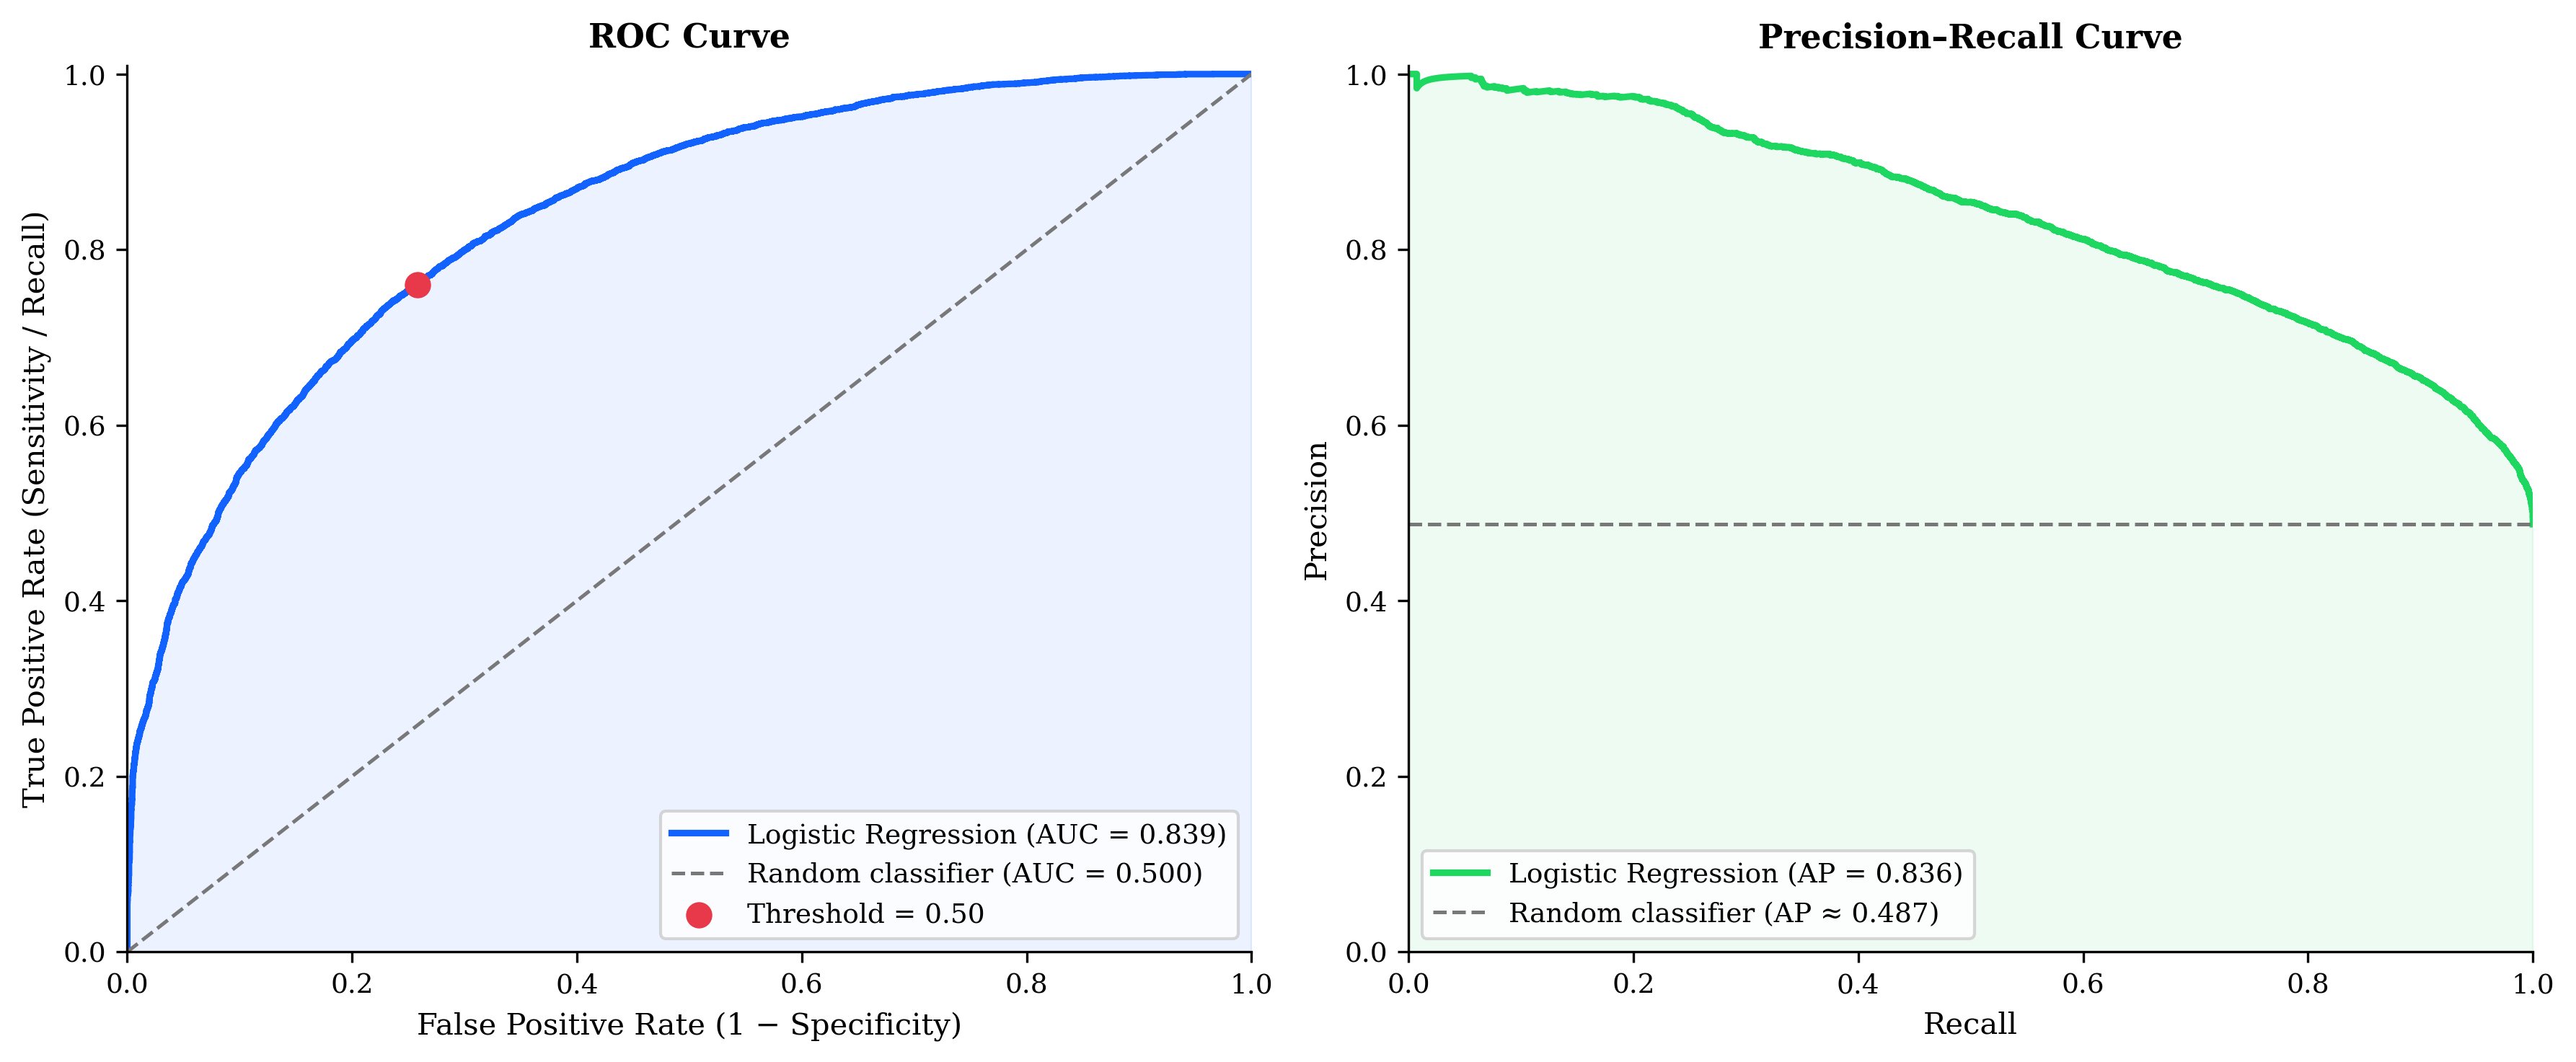
\includegraphics[width=\textwidth]{ch5_roc_pr.png}
    \caption{Left: ROC curve for logistic regression on the test set (AUC = 0.839). The dashed diagonal represents a random classifier.}
    \label{fig:ch5_roc_pr}
\end{figure}
 
\textbf{Calibration.} Figure~\ref{fig:ch5_calibration} shows a calibration plot comparing predicted probabilities to observed frequencies in ten equal-width bins. The model is reasonably well-calibrated in the middle range, with slight overconfidence at the tails—a common behavior in logistic regression when training-set probabilities are pushed toward 0 or 1 by extreme predictor values.
 
\begin{figure}[H]
    \centering
    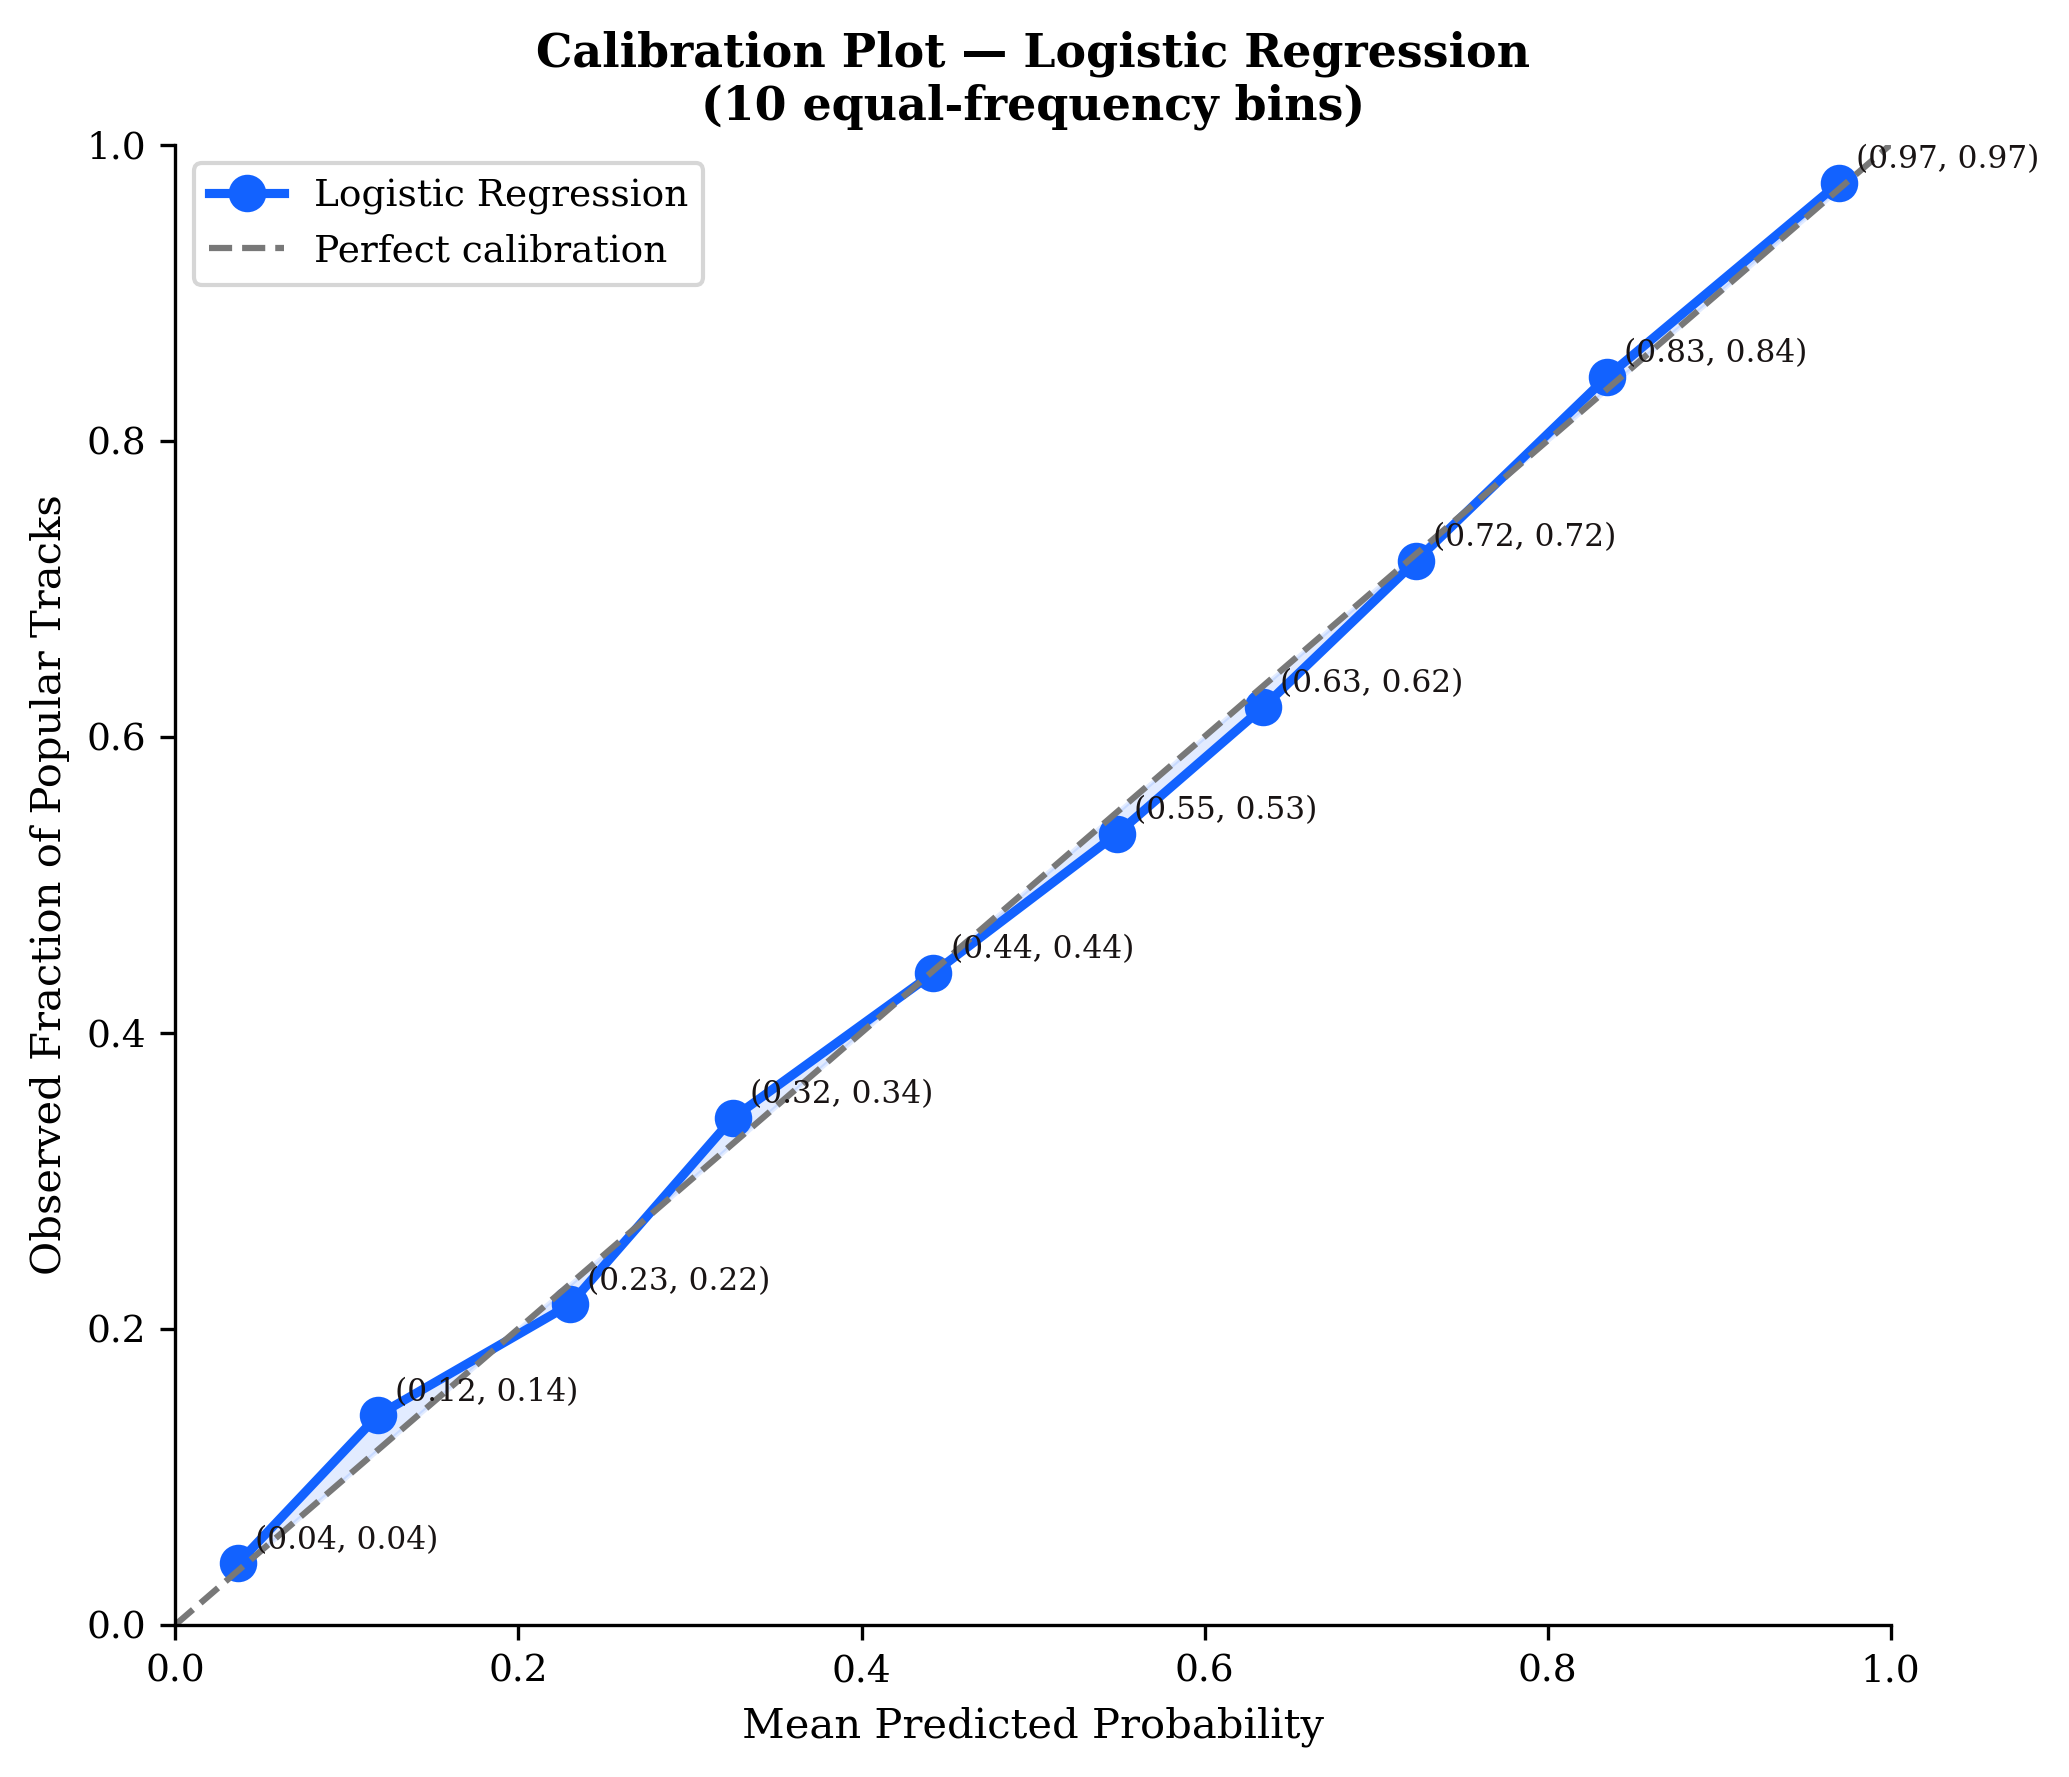
\includegraphics[width=0.75\textwidth]{ch5_calibration.png}
    \caption{Calibration plot for logistic regression. Each point represents the mean predicted probability vs.\ observed popularity rate in one of ten equal-frequency bins.}
    \label{fig:ch5_calibration}
\end{figure}
 
\textbf{Threshold analysis.} the threshold sensitivity described above shows how accuracy, precision, and recall change as the classification threshold is varied. The default threshold of 0.50 provides a good precision-recall tradeoff for this balanced problem. A label-conscious stakeholder could lower the threshold to 0.40 to recover 83.2\% of popular tracks at the cost of reduced precision.
 
 
\section{Findings}
 
Figure~\ref{fig:ch5_prob_dist} shows the distribution of predicted probabilities for popular and not-popular tracks. The two distributions separate reasonably well, with the popular class shifted toward higher predicted probabilities, but with substantial overlap in the 0.3--0.7 range, confirming that a meaningful fraction of tracks are genuinely ambiguous.
 
\begin{figure}[H]
    \centering
    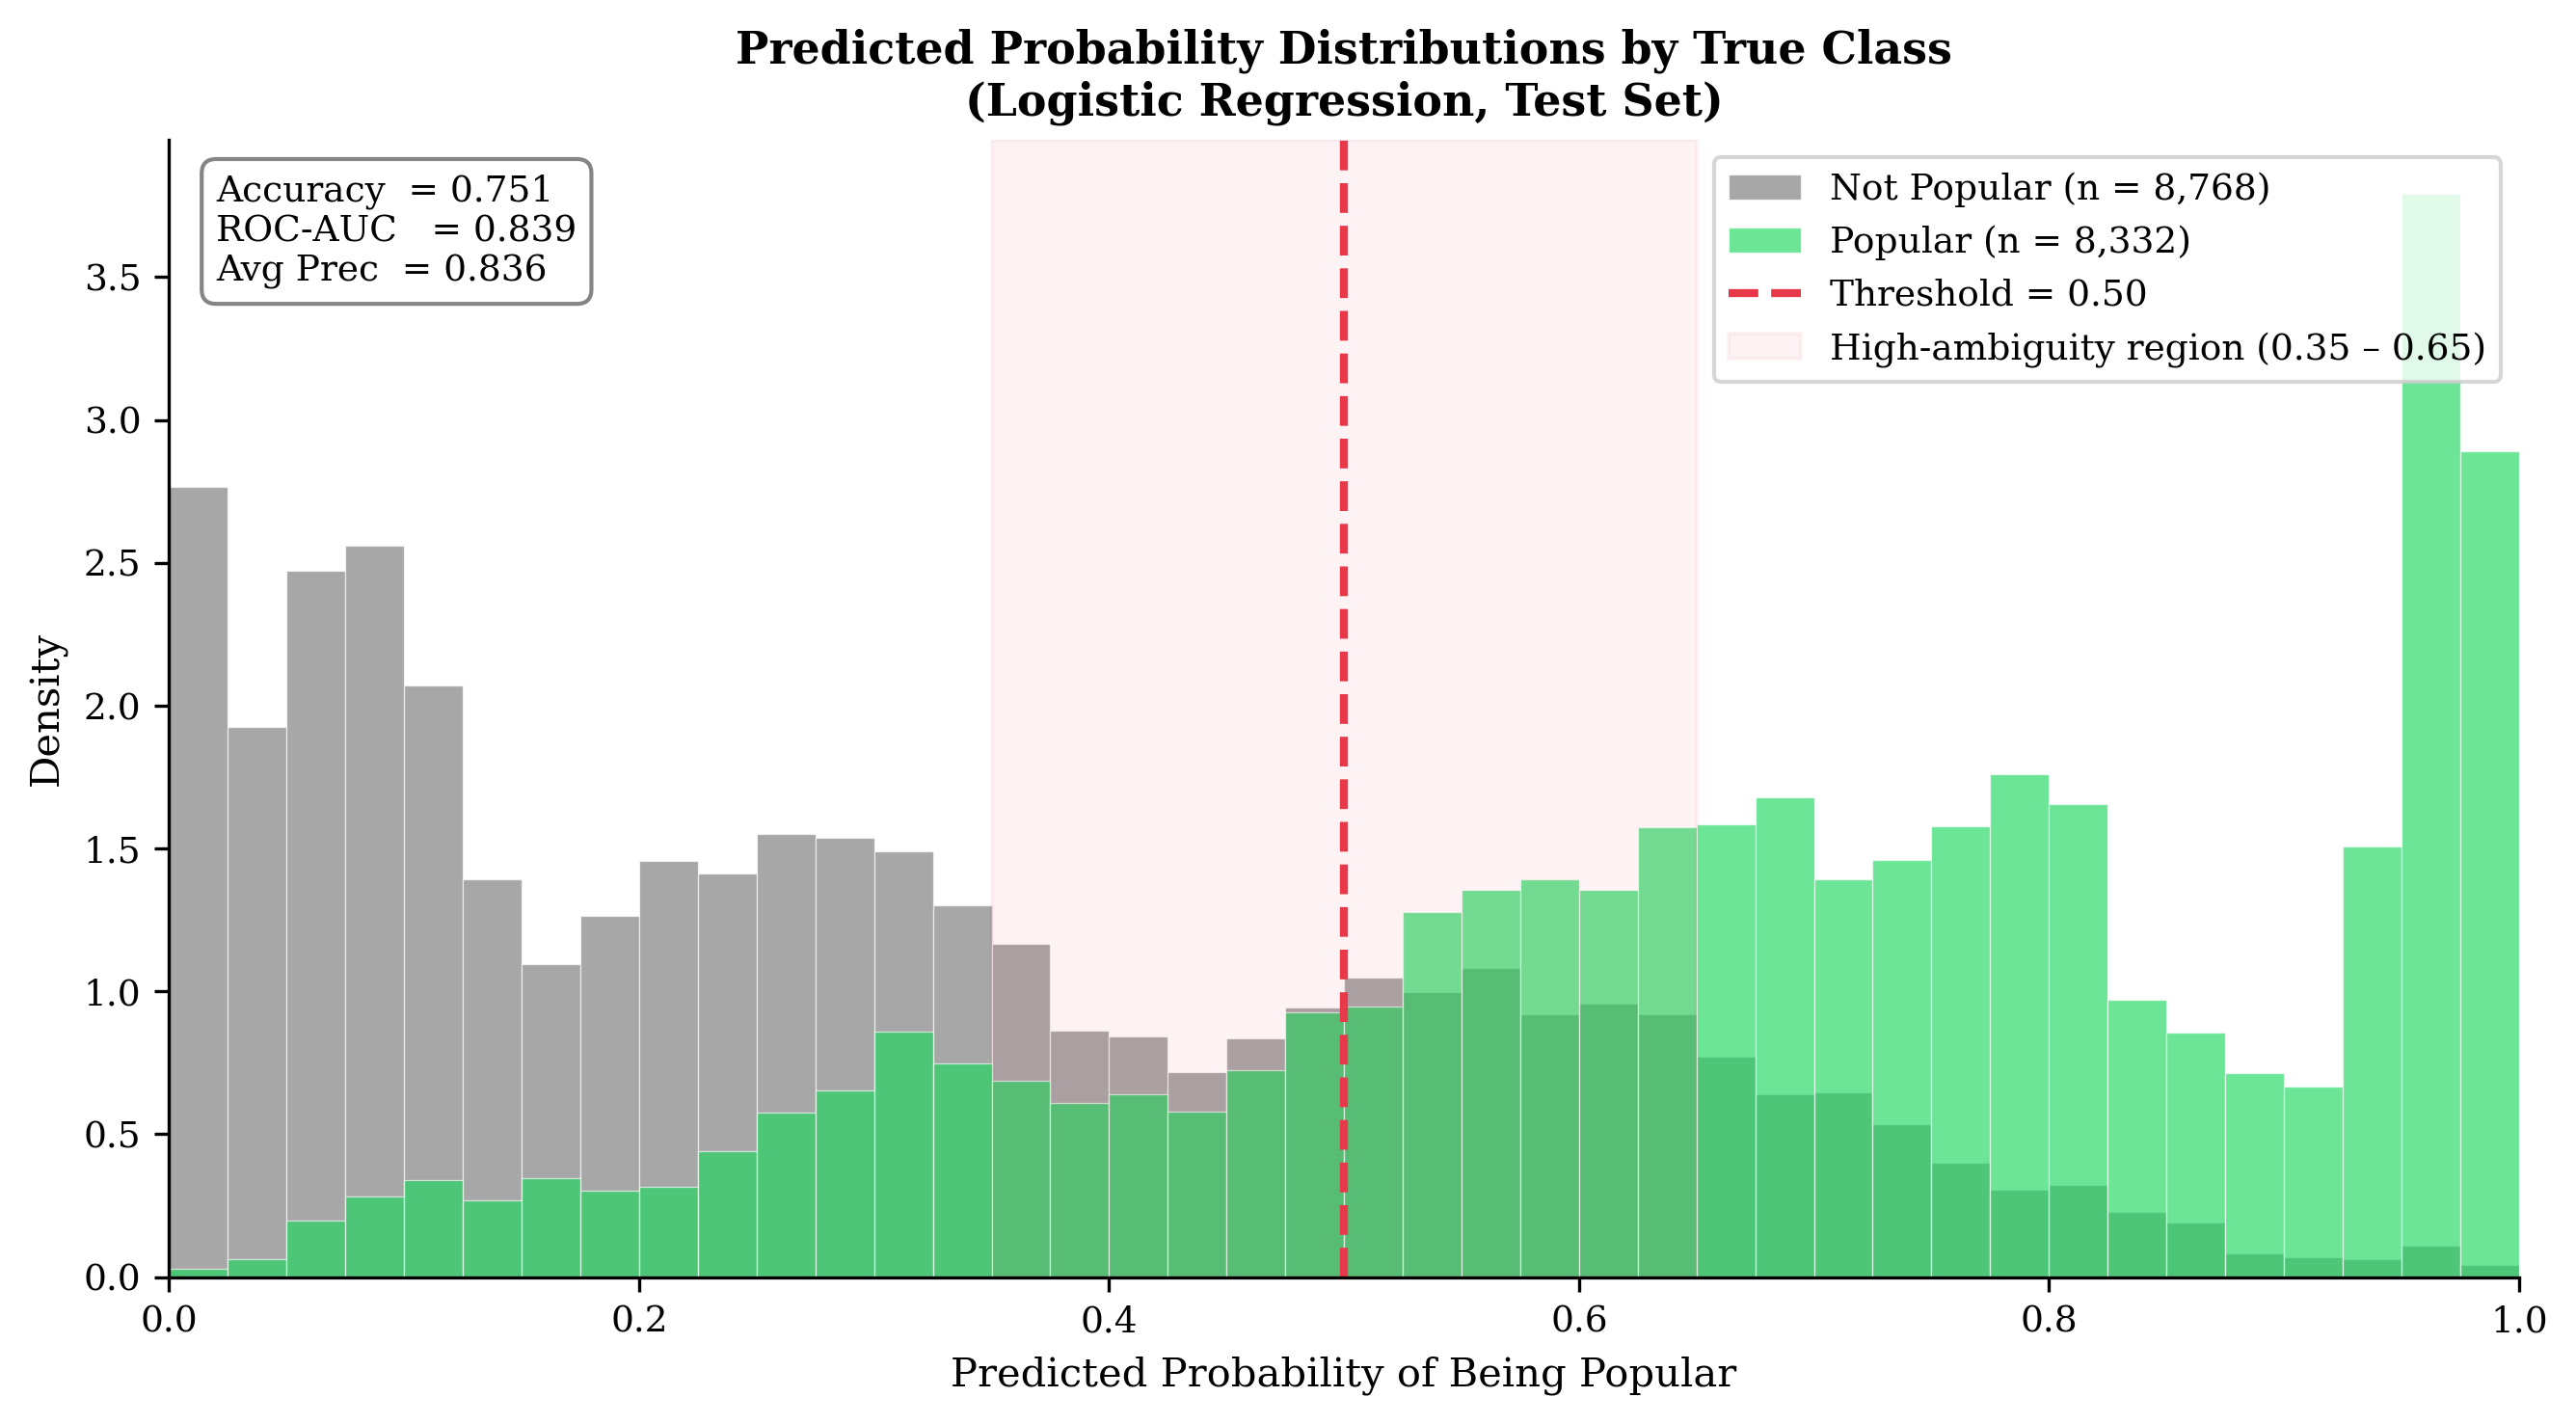
\includegraphics[width=0.85\textwidth]{ch5_prob_dist.png}
    \caption{Distribution of predicted probabilities from logistic regression, split by true class. Green = truly popular tracks and gray = truly not popular.}
    \label{fig:ch5_prob_dist}
\end{figure}
 
The model achieves 75.1\% accuracy on a near-balanced classification problem, whereas the null baseline achieves only 51.3\%. The ROC-AUC of 0.839 indicates that the model correctly ranks a randomly selected popular track above a randomly selected unpopular track 83.9\% of the time. Adding genre to the audio-feature-only model raises the AUC from 0.606 to 0.839, confirming that genre is the dominant predictor in the linear framework.
 
\chapter{Resampling Methods: Cross-Validation and Bootstrap}

\section{The Question}
 
How stable and trustworthy are the performance estimates and coefficient estimates produced? A model evaluated on a single held-out set yields a single number, but that number can be lucky or unlucky depending on which observations are included in the test set. This chapter asks two related questions, how consistent is the MLR model's predictive accuracy across different partitions of the training data, using $k$-fold cross-validation with several values of $k$, and how wide are the uncertainty intervals around the key regression coefficients from Chapter 4, using the nonparametric bootstrap?
 
\section{Method in Brief}
 
\textbf{Cross-validation} repeatedly splits the training data into $k$ complementary folds, trains the model on $k-1$ folds, and evaluates on the held-out fold. Averaging across all $k$ evaluations gives a low-variance estimate of out-of-sample error that uses the full training set rather than a single partition.
 
\textbf{The bootstrap} draws $B$ random samples of size $n$ with replacement from the training data, fits the model on each resample, and records the statistic of interest. The spread of these $B$ estimates quantifies sampling uncertainty without any distributional assumptions.
 
\section{Why This Method?}
 
Both methods address a fundamental problem in model evaluation. A single train/test split gives an estimate of generalization error that is itself a random variable. Cross-validation reduces the variance of that estimate by averaging over many splits. The bootstrap provides confidence intervals for any statistic, such as coefficients, $R^2$, and RMSE, without requiring the normality assumptions that underpin closed-form standard errors. Together they turn single-number summaries into honest uncertainty quantifications.
 
\section{Data Setup}
 
\begin{itemize}
    \item \textbf{Cross-validation target}: the full 139-predictor MLR model from Chapter 4. All CV is performed on the training set only ($n_{\text{train}} = 79{,}799$). 
    
    \item \textbf{Bootstrap target}: eight interpretable non-genre predictors (danceability, energy, loudness, speechiness, acousticness, instrumentalness, valence, explicit), plus the test-set $R^2$ of the full MLR model.
    \item \textbf{Bootstrap implementation}: $B = 2{,}000$ resamples on an 8{,}000-row subsample of the training set (drawn once without replacement). The subsample is used for computational tractability; since $n = 8{,}000 \gg p = 139$, it is sufficiently large to yield reliable estimates.
    \item \textbf{Bootstrap interval type}: percentile interval, which makes no assumption about the shape of the sampling distribution.
\end{itemize}
 
\section{Analysis}
 
\subsection{Cross-Validation: Comparing $k$ Values}
 
Table~\ref{tab:ch6_cv_rmse} shows the 5-fold, 10-fold, and 20-fold CV results for the MLR regression model. The mean RMSE is almost identical across all values of $k$, confirming that the model's generalization error is not sensitive to the choice of $k$. The standard deviation across folds increases with $k$, which is the expected bias-variance tradeoff of cross-validation. Higher $k$ means each training fold is larger, but the fold estimates are more correlated (higher variance between folds).
 
\begin{table}[H]
\centering
\caption{$k$-fold cross-validation results for the MLR model (regression, RMSE) and logistic regression model (classification, ROC-AUC) on the training set ($n = 79{,}799$). All CV performed with shuffled folds and \texttt{random\_state = 42}.}
\label{tab:ch6_cv_rmse}
\begin{tabular}{lrrrr}
\toprule
\multirow{2}{*}{\textbf{$k$}} & \multicolumn{2}{c}{\textbf{MLR --- RMSE}} & \multicolumn{2}{c}{\textbf{Logistic --- AUC}} \\
\cmidrule(lr){2-3} \cmidrule(lr){4-5}
& \textbf{Mean} & \textbf{Std} & \textbf{Mean} & \textbf{Std} \\
\midrule
3  & 19.181 & 0.006 & 0.842 & 0.002 \\
5  & 19.184 & 0.135 & 0.842 & 0.003 \\
10 & 19.177 & 0.181 & 0.842 & 0.004 \\
20 & 19.174 & 0.234 & 0.842 & 0.006 \\
\midrule
\textbf{Test set (locked)} & \textbf{19.248} & --- & \textbf{0.839} & --- \\
\bottomrule
\end{tabular}
\end{table}
 
Two observations stand out. First, the CV estimates (19.174--19.184) are slightly optimistic relative to the locked test-set RMSE (19.248). As expected, the model has seen all training data during fitting, and the CV operates within that same pool. The gap of $\approx 0.07$ RMSE units is negligible and does not suggest overfitting. Second, the logistic regression AUC remains at 0.842 across all values of $k$, with standard deviations below 0.006. This stability is a direct consequence of the large size of the training set. With nearly 80{,}000 observations, any random partition of the data produces an almost equally representative fold.
 
Figure~\ref{fig:ch6_cv_comparison} visualizes the RMSE distributions at the fold-level for $k = 5$ and $k = 10$, illustrating how the variance between folds increases with $k$ even when the mean stays constant.
 
\begin{figure}[H]
    \centering
    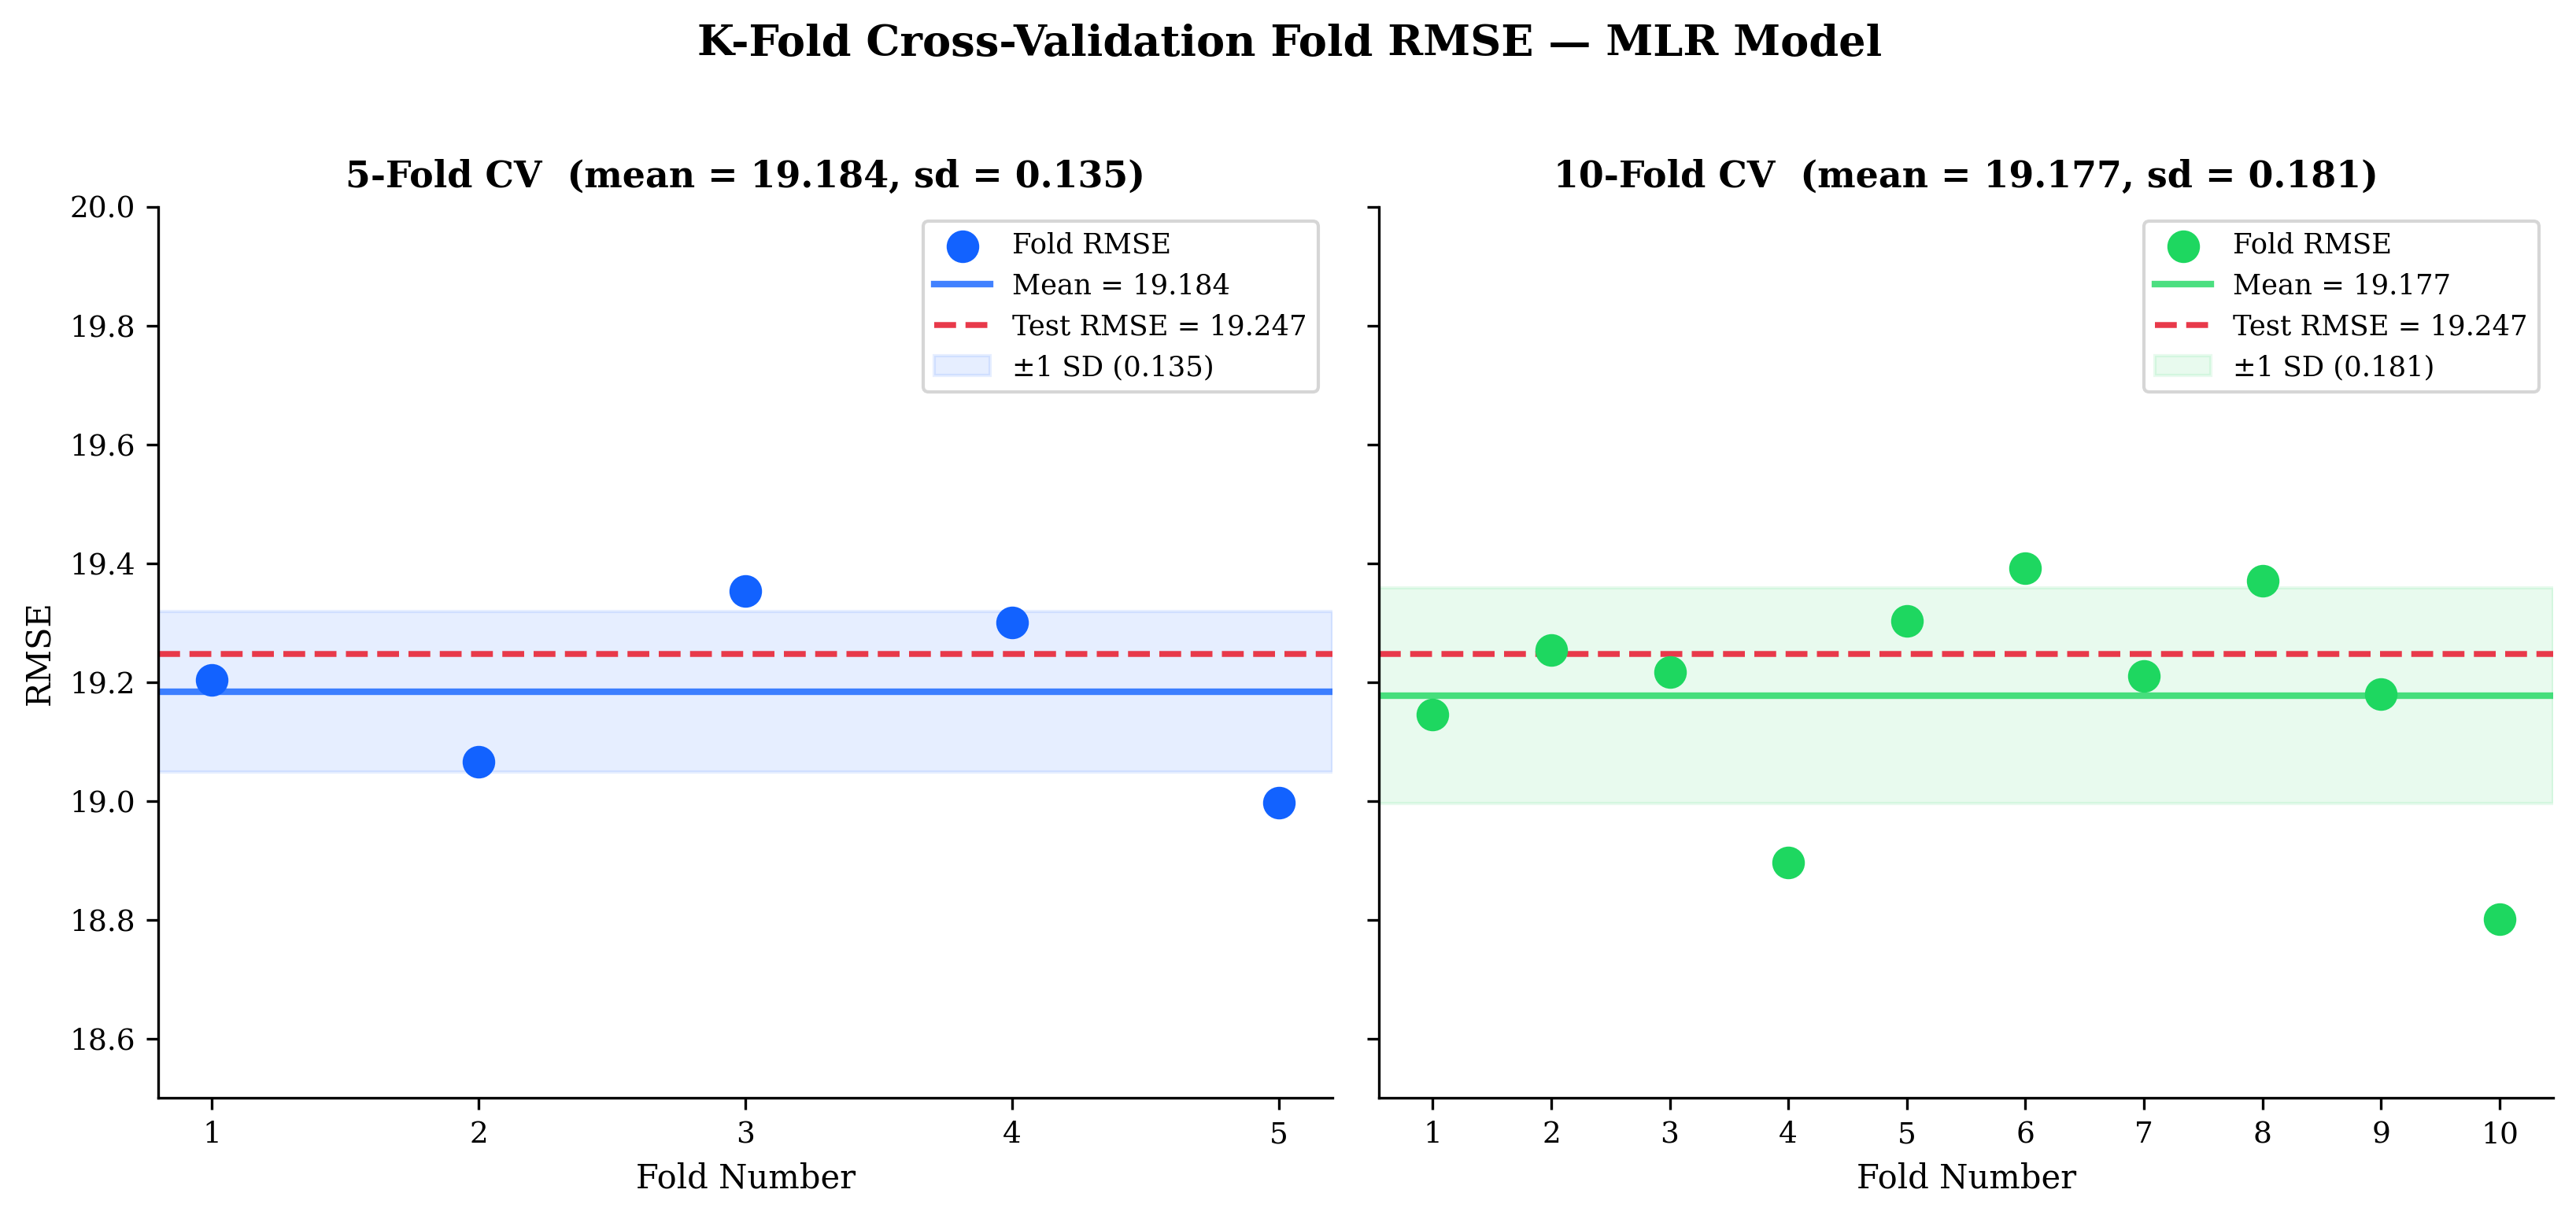
\includegraphics[width=\textwidth]{ch6_cv_comparison.png}
    \caption{Cross-validation fold RMSE distributions for $k = 5$ and $k = 10$. Each point is one fold's RMSE.}
    \label{fig:ch6_cv_comparison}
\end{figure}

\subsection{Bootstrap: Coefficient Confidence Intervals}
 
the bootstrap intervals confirm that danceability, energy, instrumentalness, valence, and explicit have intervals excluding zero (reliable nonzero effects), while loudness, speechiness, and acousticness include zero. Each interval is based on $B = 2{,}000$ resamples.
 
 
Five of the eight predictors have bootstrap intervals that exclude zero: danceability, energy, instrumentalness, valence, and explicit. These are the most reliably nonzero effects in the model. Loudness, which appeared significant in both SLR and the OLS $t$-test output of Chapter 4. Bootstrap interval that includes zero ($[-0.142,\ +1.438]$), suggesting its coefficient is more sensitive to the specific sample than the parametric $t$-test implied. Speechiness and acousticness also include zero, consistent with their lower $t$-statistics in Chapter 4.
 
Figure~\ref{fig:ch6_boot_distributions} shows the bootstrap distributions for all eight coefficients, making the width and asymmetry of each interval visible.
 
\begin{figure}[H]
    \centering
    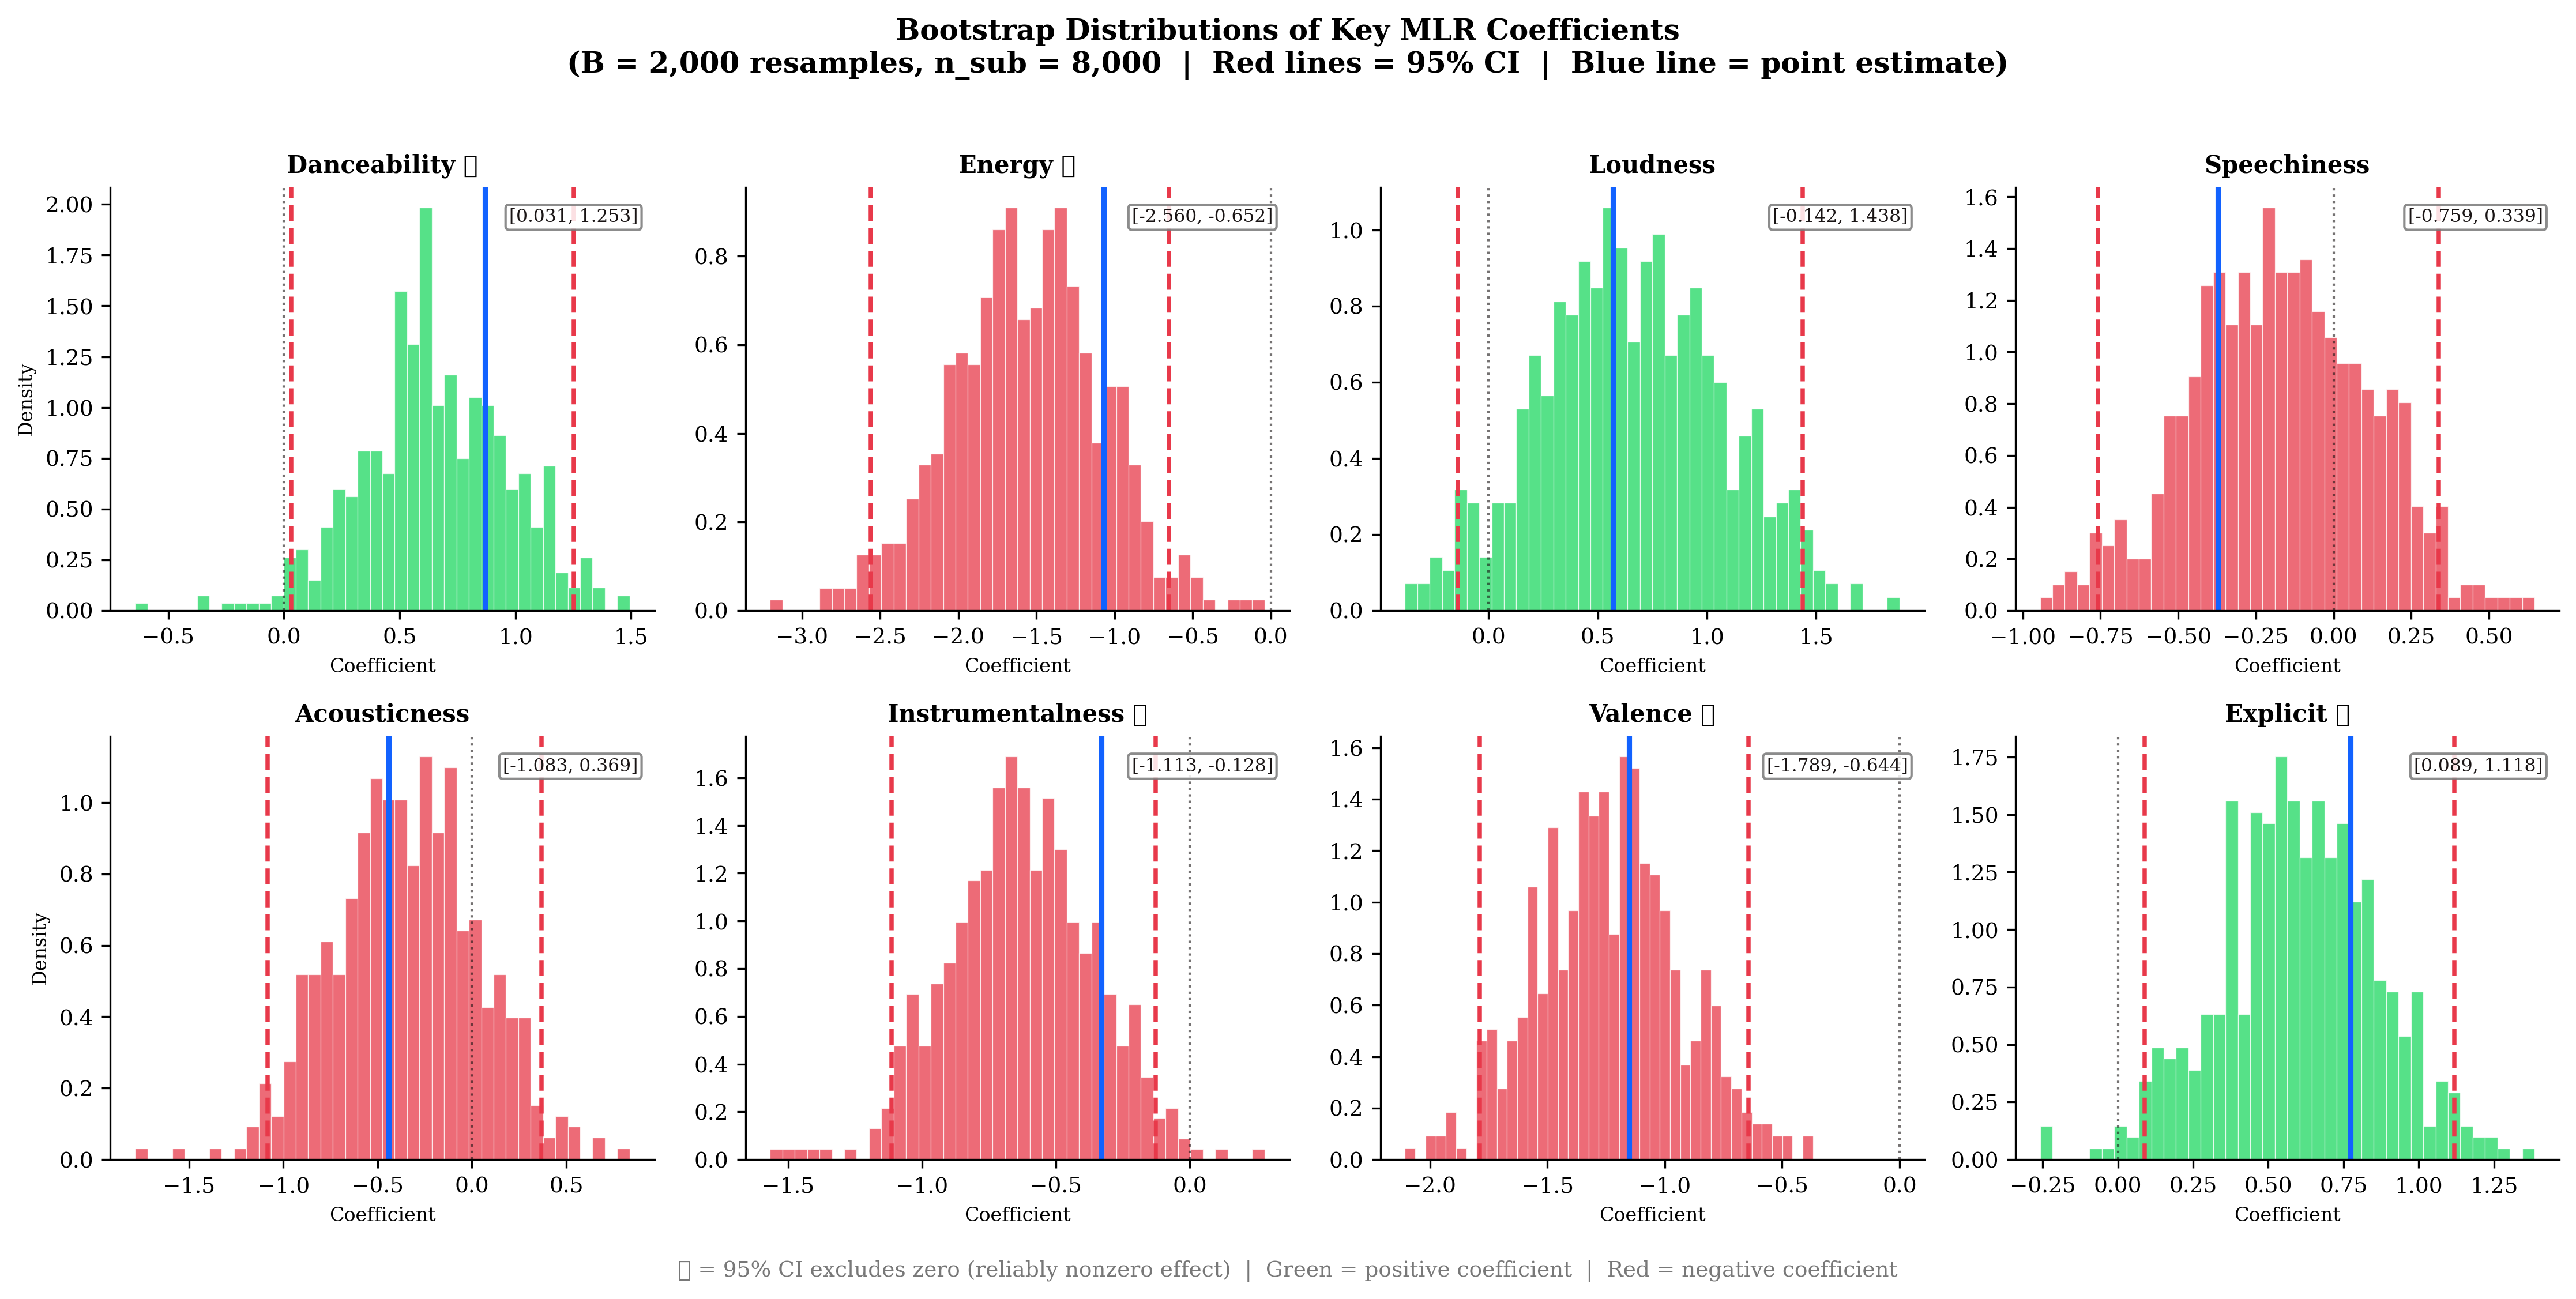
\includegraphics[width=\textwidth]{ch6_boot_distributions.png}
    \caption{Bootstrap distributions ($B = 2{,}000$ resamples) for eight key MLR coefficients. Each histogram shows the sampling distribution of the coefficient under repeated resampling.}
    \label{fig:ch6_boot_distributions}
\end{figure}
 
\subsection{Bootstrap: Test-Set $R^2$}
 
The bootstrap is also used to quantify uncertainty around the test-set $R^2$ of the full MLR model. Resampling from the test set with replacement and recomputing $R^2$ on each resample yields:
 
\begin{itemize}
    \item \textbf{Point estimate}: $R^2 = 0.259$
    \item \textbf{Bootstrap mean}: $0.263$
    \item \textbf{Bootstrap SE}: $0.016$
    \item \textbf{95\% CI}: $[0.231,\ 0.293]$
    \item \textbf{Bias}: $+0.004$
\end{itemize}
 
The $R^2$ of 0.259 is a stable estimate, even in the worst 2.5\% of bootstrap samples, it exceeds 0.231, meaning the model explains at least 23\% of popularity variance across any reasonable resampling of the test set.
 
\section{Diagnostics and Tuning}
 
Cross-validation itself is the primary diagnostic in this chapter. The key tuning decision is the choice of $k$. Given the large training set size and the negligible sensitivity to $k$ shown in Table~\ref{tab:ch6_cv_rmse}, five-fold CV is adopted as the standard for all subsequent chapters. It provides a good balance: it is fast enough to run within hyperparameter search loops, while yielding a mean estimate whose variance is low enough to reliably rank models.
 
\section{Findings}
 
The MLR model's 5-fold CV RMSE of $19.184 \pm 0.135$ closely matches the test-set RMSE of 19.248, confirming that the single-split estimate from Chapter 4 was not a statistical accident. The bootstrap reinforces this: the 95\% CI for the test $R^2$ is $[0.231,\ 0.293]$, entirely above zero and below the 0.30 ceiling that Chapter 14 will show the ensemble methods approach. Coefficient-level bootstrap results identify valence and energy as the most precisely estimated negative effects, and danceability and explicit as the most precisely estimated positive effects and findings that will recur in the variable importance plots of Chapters 9 and 12.
 
\chapter{Regularization: Ridge and Lasso}
 
\section{The Question}
 
Can penalized regression improve on the ordinary least squares model from Chapter 4? With 139 predictors and nearly 80{,}000 training observations, the ratio of observations to parameters is very favorable, so overfitting is unlikely. Some predictors may carry redundant signal, particularly the 113 genre dummies, and shrinking or zeroing their coefficients might reduce test error. This chapter asks whether ridge or lasso regularization yields a meaningful improvement over OLS, and, if so, which predictors are retained by lasso's variable selection.
 
\section{Method in Brief}
 
Ridge regression adds a penalty proportional to the \textit{sum of squared} coefficients to the OLS loss function. This shrinks all coefficients toward zero but never sets any exactly to zero. Lasso adds a penalty proportional to the \textit{sum of absolute} coefficients, which produces exact zeros and therefore performs automatic variable selection. In both cases, the penalty strength is controlled by a hyperparameter $\alpha$; at $\alpha = 0$, both methods reduce to OLS; as $\alpha \to \infty$, all coefficients are driven to zero.
 
\section{Why This Method?}
 
Regularization guards against overfitting when the predictor space is large relative to the training set, and provides a principled way to rank predictors by survival under increasing penalty. Even if the full OLS model does not overfit here, lasso variable selection offers a path to a parsimonious model that uses far fewer than 139 predictors, which is useful for interpretability and deployment. Ridge is included as a companion, because it handles correlated predictors (energy, loudness, acousticness) more gracefully than lasso.
 
\section{Data Setup}
 
\begin{itemize}
    \item \textbf{Response}: \texttt{popularity} (continuous).
    \item \textbf{Predictors}: Same 139-column design matrix as Chapter 4. All predictors standardized.
    \item \textbf{Alpha grid}: 100 values log-spaced from $10^{-2}$ to $10^{4}$.
    \item \textbf{Tuning}: 5-fold cross-validation on the training set via \texttt{RidgeCV} and \texttt{LassoCV}. The $\alpha$ minimizing CV RMSE is selected.
    \item \textbf{Split}: Same 70/15/15 stratified split.
\end{itemize}
 
\section{Analysis}
 
\subsection{Hyperparameter Selection}
 
Figure~\ref{fig:ch7_cv_curves} shows the 5-fold CV RMSE as a function of $\log_{10}(\alpha)$ for both ridge and lasso. Both curves are nearly flat across a wide range of small $\alpha$ values before rising sharply as regularization becomes too strong. The optimal $\alpha$ for ridge is 14.17. For lasso, it is 0.01, the smallest value on the grid, indicating that any amount of $\ell_1$ shrinkage beyond this minimum value slightly increases the CV error.
 
\begin{figure}[H]
    \centering
    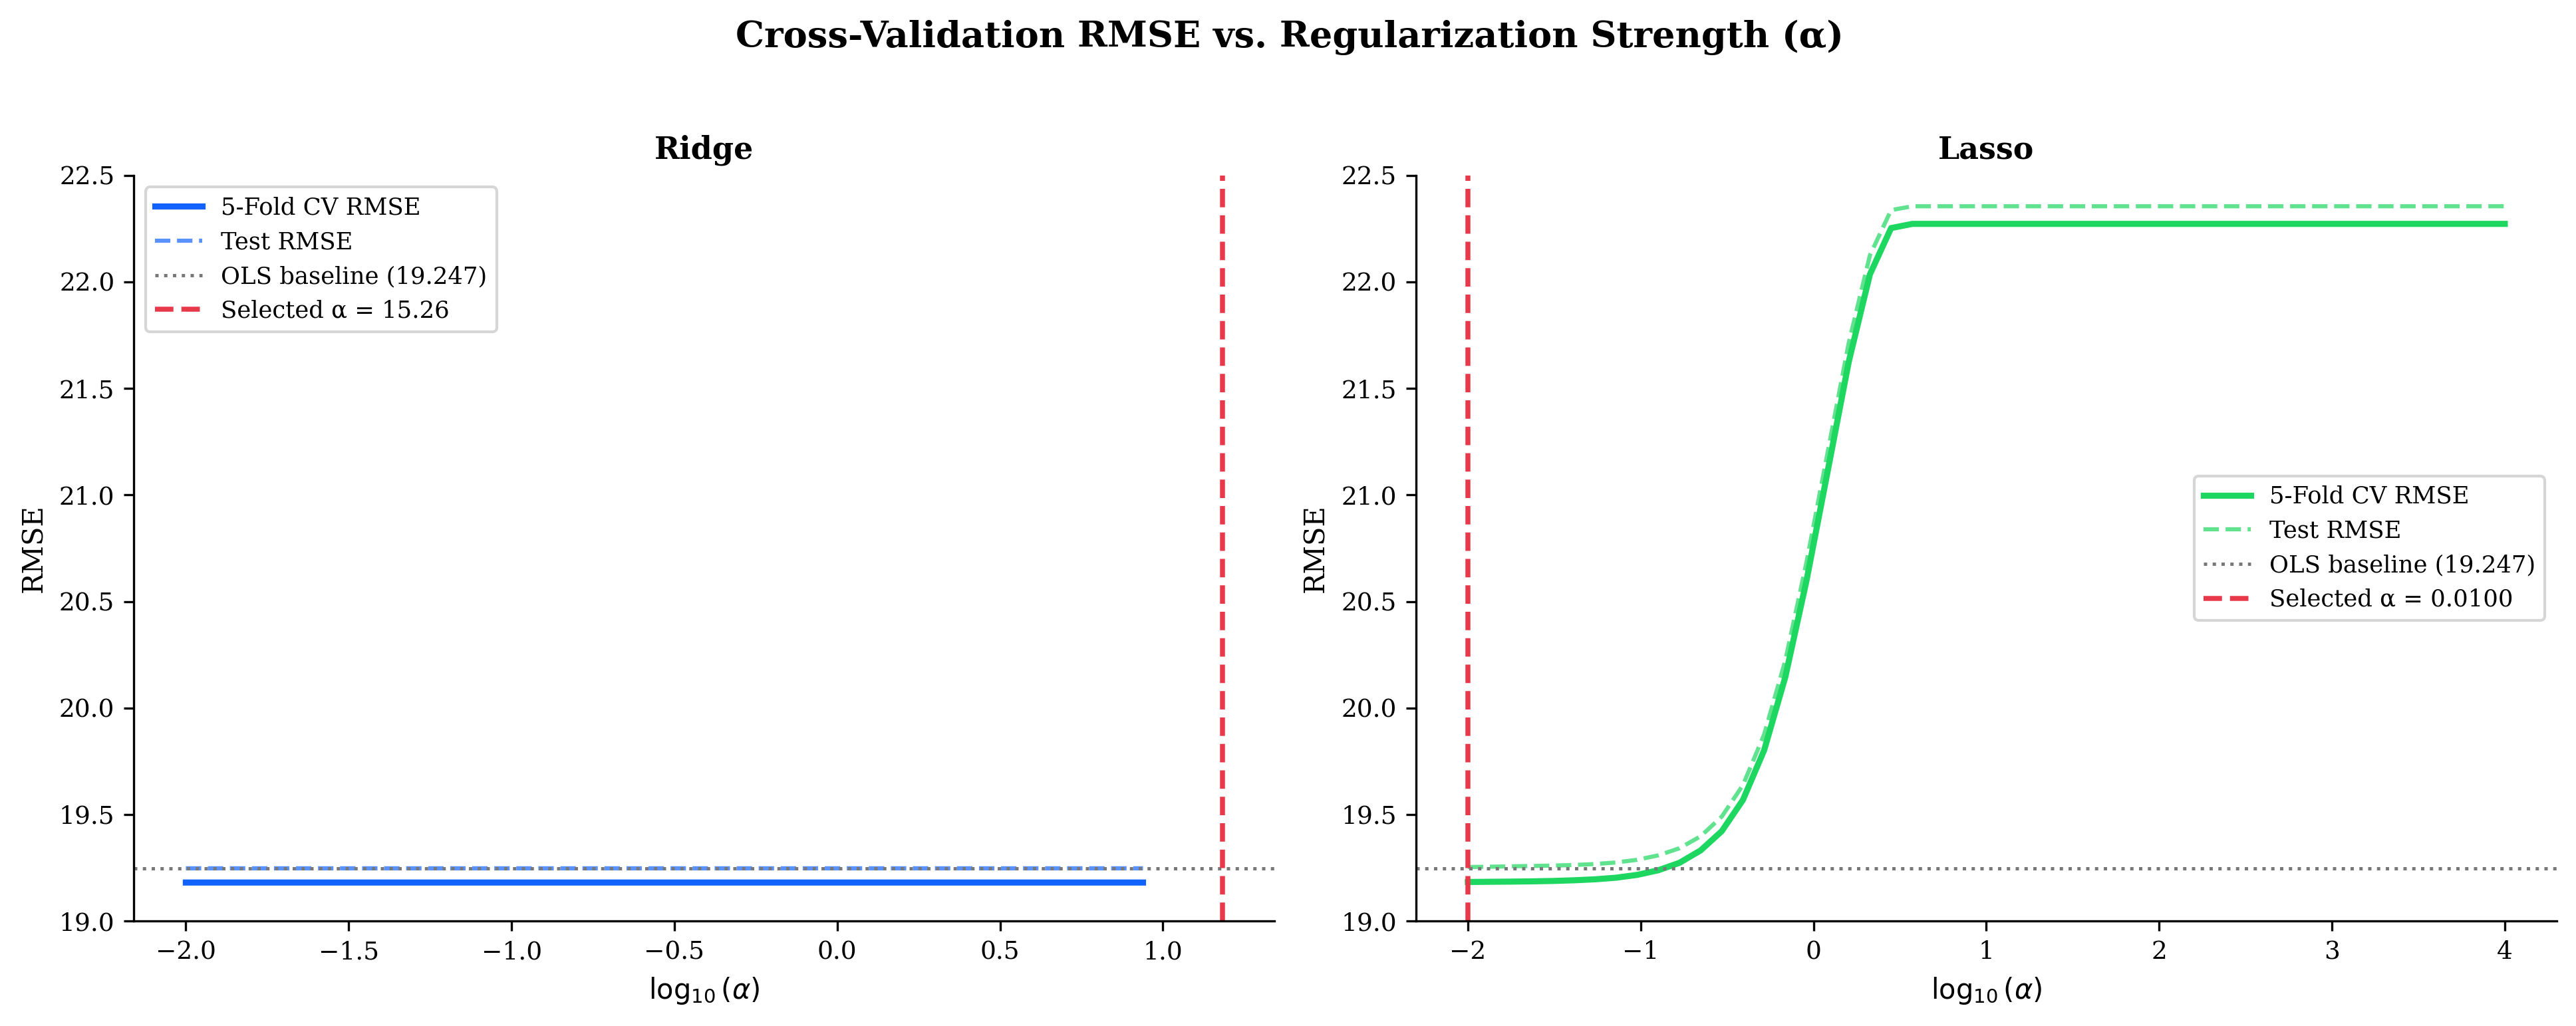
\includegraphics[width=\textwidth]{ch7_cv_curves.png}
    \caption{5-fold CV RMSE vs.\ $\log_{10}(\alpha)$ for ridge (left) and lasso (right). The vertical dashed line marks the selected $\alpha$ in each panel.}
    \label{fig:ch7_cv_curves}
\end{figure}
 
\subsection{Coefficient Paths}
 
Figure~\ref{fig:ch7_coef_paths} shows how each coefficient evolves as $\alpha$ increases, the regularization path for both methods. For the ridge, all coefficients shrink smoothly and continuously toward zero, never reaching it exactly. For the lasso, coefficients reach zero at different rates depending on their magnitude.
 
\begin{figure}[H]
    \centering
    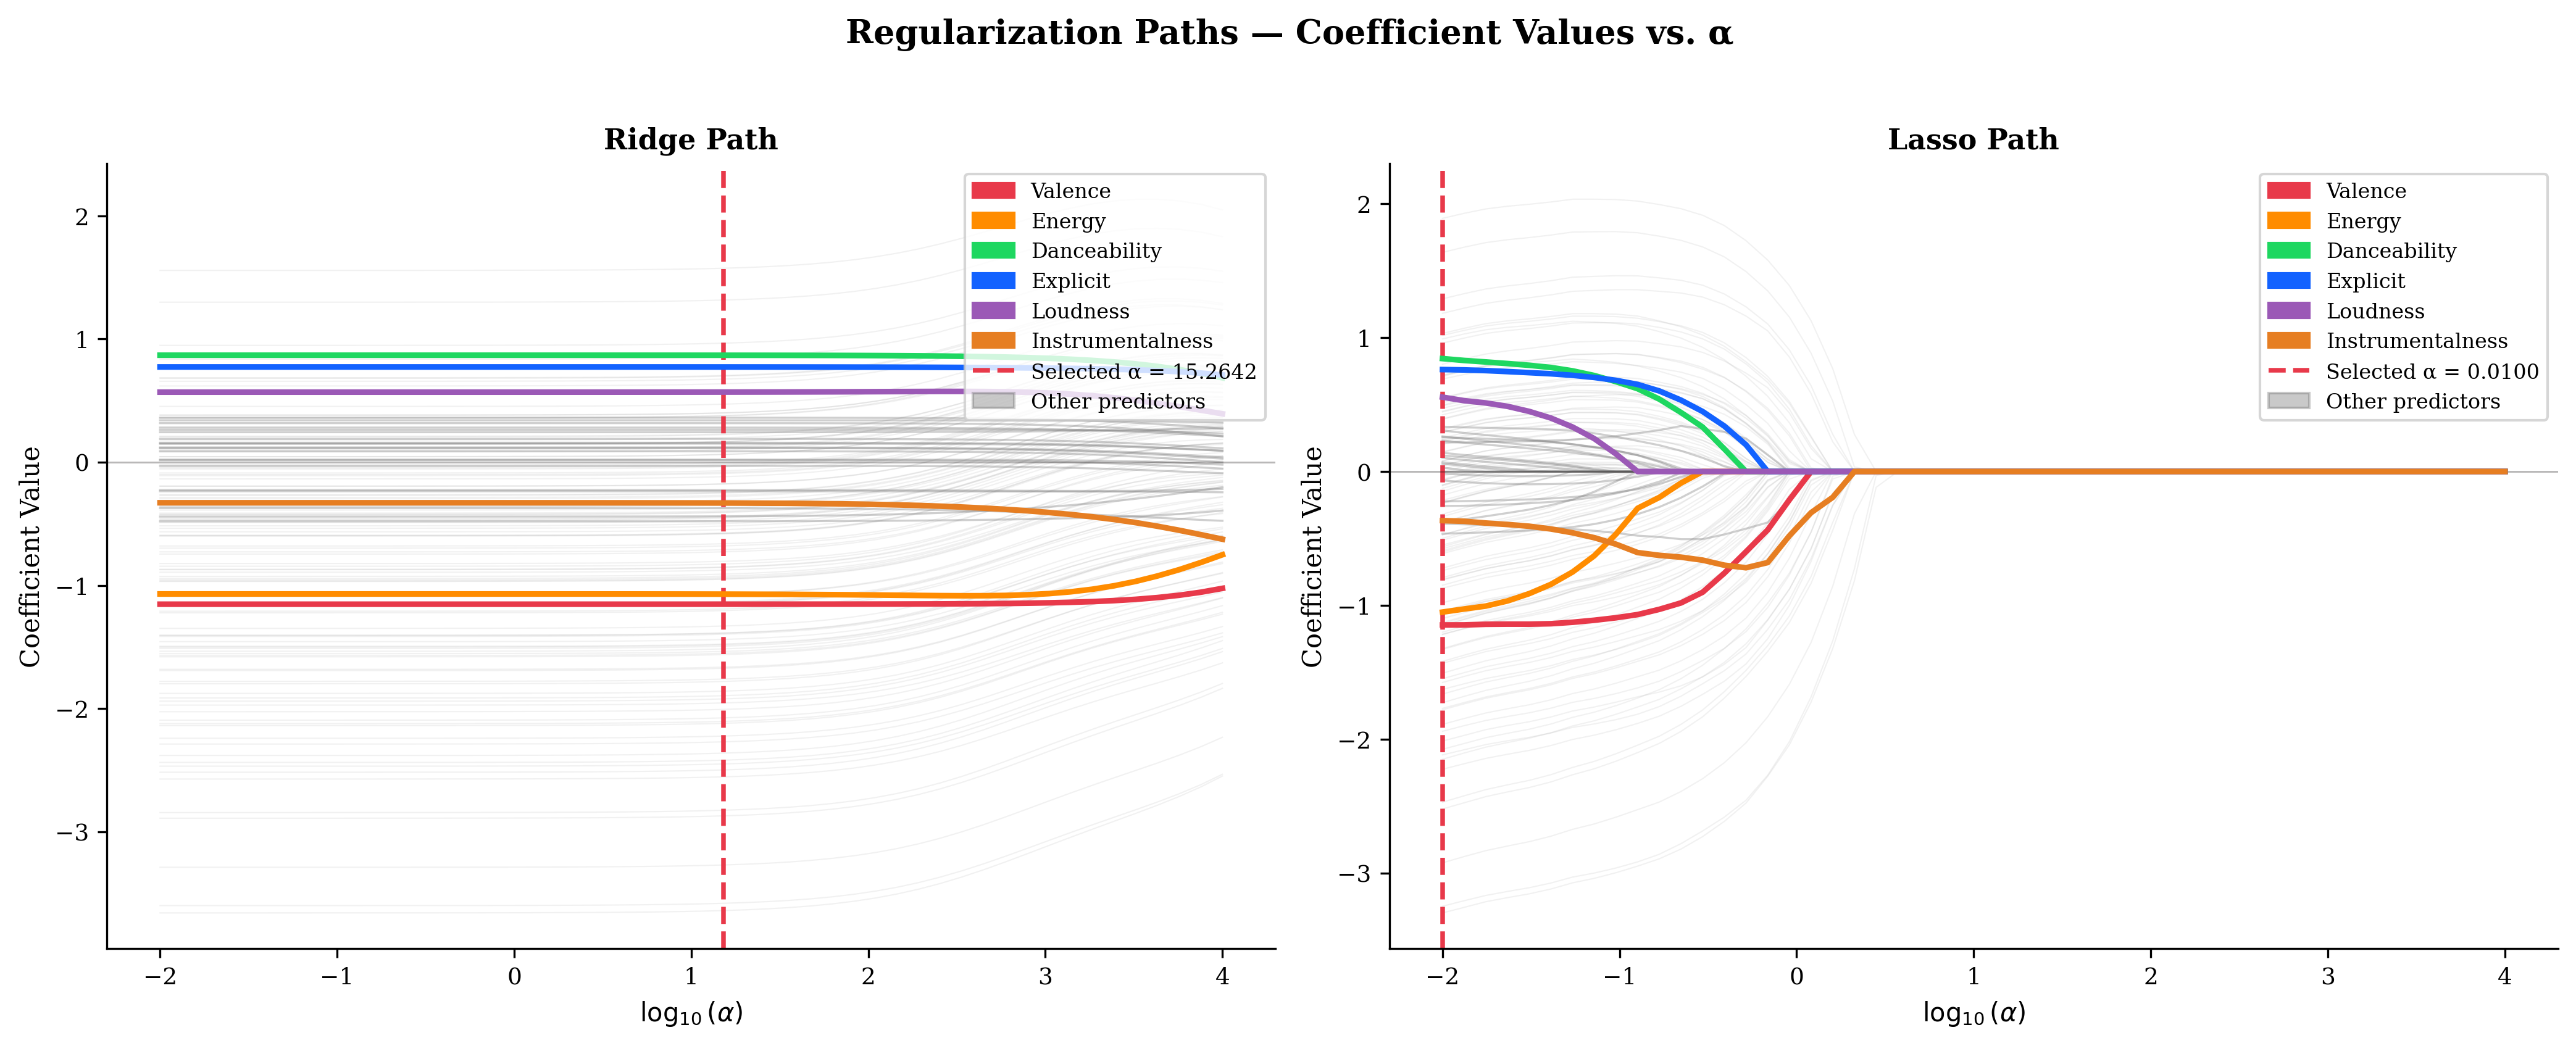
\includegraphics[width=\textwidth]{ch7_coef_paths.png}
    \caption{Regularization paths for ridge (left) and lasso (right). Each line represents one predictor's coefficient across the $\alpha$ grid.}
    \label{fig:ch7_coef_paths}
\end{figure}
 
\subsection{Variable Selection}
 
At the selected $\alpha = 0.01$, lasso retains 137 of 139 predictors, zeroing out only two: \texttt{ts\_5} (time signature = 5, an extremely rare meter present in fewer than 0.5\% of tracks) and \texttt{genre\_techno}. This near-complete retention confirms that essentially all predictors carry at least marginal signal once the model is fit on 79{,}799 observations. The lasso only becomes meaningfully selective at $\alpha \geq 0.5$, by which point it has already introduced substantial bias, and the test RMSE has risen from 19.25 to 19.84.
 
Table~\ref{tab:ch7_lasso_survival} summarizes how many predictors survive lasso at five $\alpha$ values, alongside the corresponding test RMSE.
 
\begin{table}[H]
\centering
\caption{Lasso variable selection at increasing penalty strengths. At the CV-selected $\alpha = 0.01$, only 2 predictors are zeroed out.}
\label{tab:ch7_lasso_survival}
\begin{tabular}{rrrr}
\toprule
\textbf{$\alpha$} & \textbf{Total nonzero} & \textbf{Genre nonzero} & \textbf{Test RMSE} \\
\midrule
0.01 (selected) & 137 & 112 & 19.254 \\
0.05            & 132 & 110 & 19.266 \\
0.10            & 125 & 106 & 19.290 \\
0.50            &  78 &  73 & 19.840 \\
1.00            &  37 &  34 & 20.849 \\
\bottomrule
\end{tabular}
\end{table}
 
\section{Diagnostics and Tuning}
 
\textbf{Comparison with OLS.} Table~\ref{tab:ch7_model_comparison} places ridge and lasso alongside OLS on the same test set. All three models achieve essentially identical test $R^2$ and RMSE. The differences are in the fourth decimal place.
 
\begin{table}[H]
\centering
\caption{Performance comparison: OLS (Chapter 4), ridge ($\alpha = 14.17$), and lasso ($\alpha = 0.01$) on the locked test set. All metrics rounded to three decimal places.}
\label{tab:ch7_model_comparison}
\begin{tabular}{lrrr}
\toprule
\textbf{Model} & \textbf{Train $R^2$} & \textbf{Test $R^2$} & \textbf{Test RMSE} \\
\midrule
OLS (Chapter 4)         & 0.261 & 0.259 & 19.248 \\
Ridge ($\alpha = 14.17$) & 0.261 & 0.259 & 19.248 \\
Lasso ($\alpha = 0.01$)  & 0.261 & 0.258 & 19.254 \\
\bottomrule
\end{tabular}
\end{table}
 
\textbf{Coefficient shrinkage.} Figure~\ref{fig:ch7_coef_compare} shows a direct comparison of OLS, ridge, and lasso coefficients for the 15 largest non-genre predictors. Ridge coefficients are nearly indistinguishable from OLS at $\alpha = 14.17$, confirming that the penalty is mild. Lasso coefficients are similarly close to those of OLS, with the smallest predictors exhibiting marginally greater shrinkage.
 
\begin{figure}[H]
    \centering
    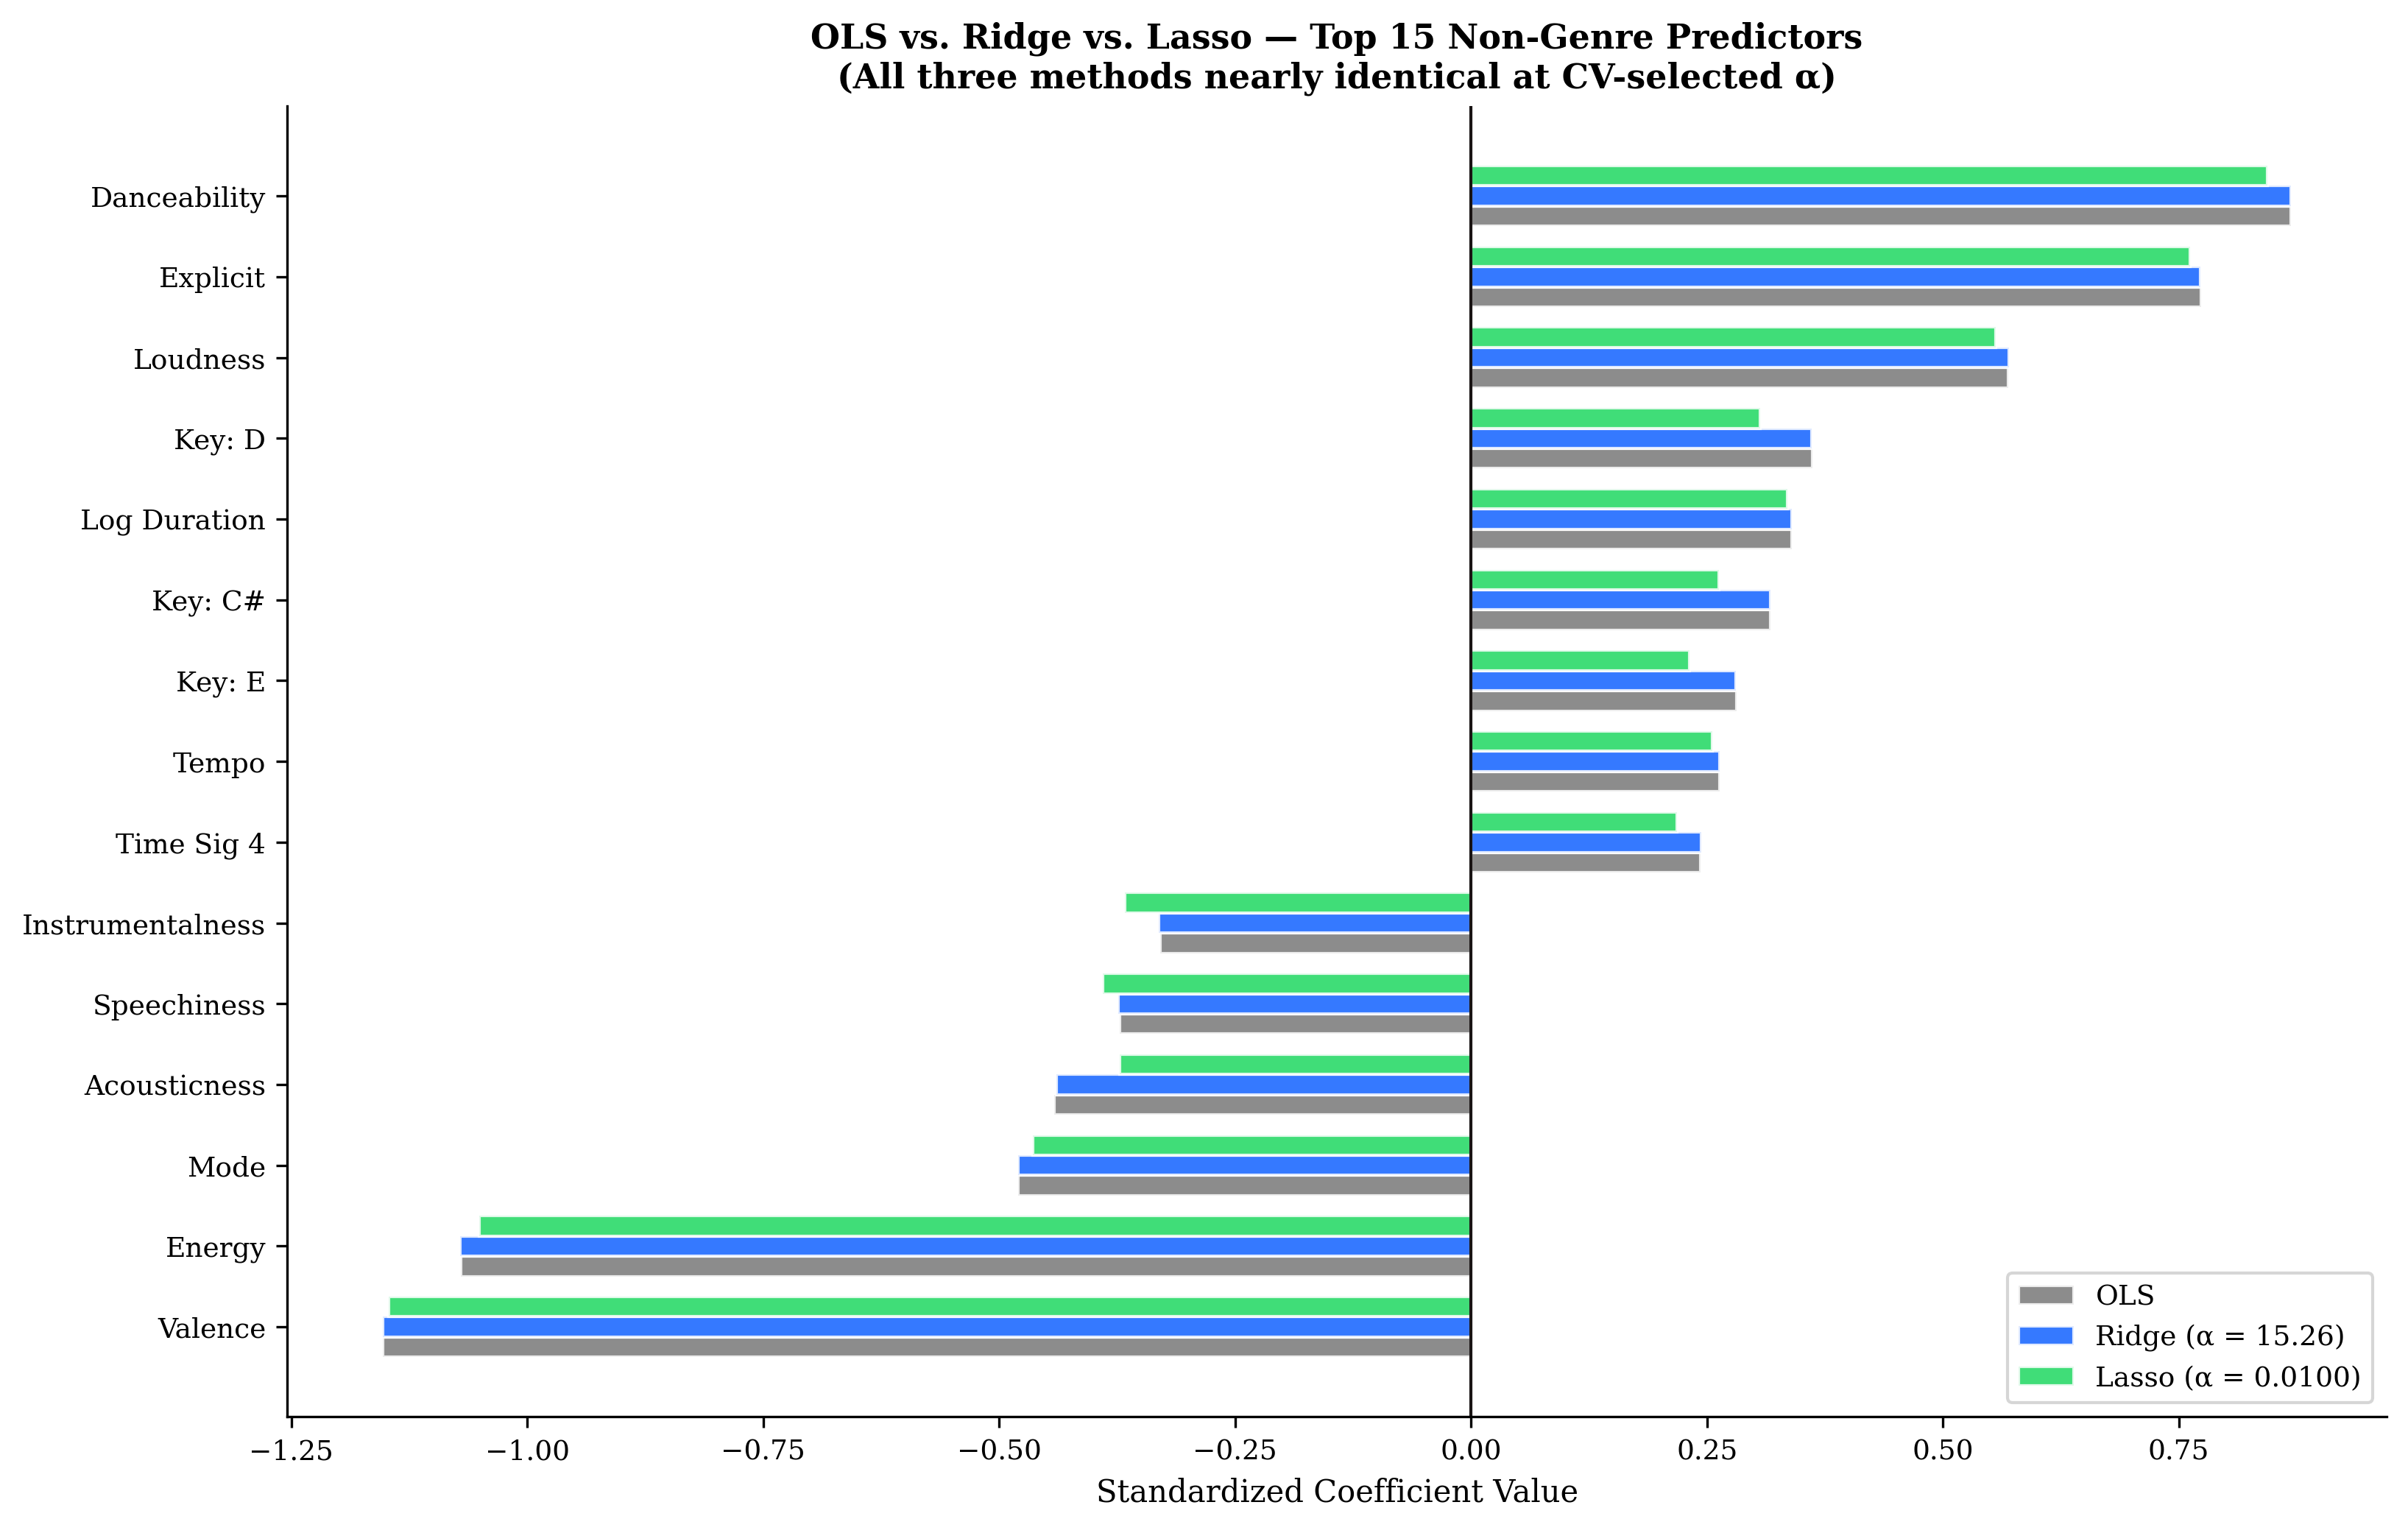
\includegraphics[width=0.88\textwidth]{ch7_coef_compare.png}
    \caption{Coefficient comparison across OLS, ridge, and lasso for the 15 largest non-genre predictors. The three methods produce nearly identical estimates, reflecting the large training set and the mild optimal penalties selected by cross-validation.}
    \label{fig:ch7_coef_compare}
\end{figure}
 
\section{Findings}
 
Ridge regression and lasso converge to the OLS solution at their CV-selected penalties. The lasso retains 137 of the 139 predictors and improves the RMSE test by 0.006 over OLS, a difference of 0.03\%, which is statistically and practically negligible. The two zeroed predictors (\texttt{ts\_5} and \texttt{genre\_techno}) are dummy variables for the rare categories, with near-zero OLS coefficients, making their removal unsurprising.
 
The non-genre predictors that survive with the largest lasso coefficients are, in order: valence ($-1.147$), energy ($-1.051$), danceability ($+0.844$), explicit ($+0.762$), and loudness ($+0.556$). This ordering is identical to the Chapter 4 MLR ranking and is consistent with the bootstrap results in Chapter 6, in which these same five predictors had zero-excluding confidence intervals. The lasso has independently confirmed the bootstrap's identification of the most reliable predictors.
 
\chapter{Decision Trees}
 
\section{The Question}
 
Can a single decision tree, which makes no linearity assumption and can capture arbitrary splits in the feature space, outperform the multiple linear regression baseline from Chapter 4? And does it learn the same genre-dominated structure, or does it discover genuinely different patterns? This chapter fits both a \textit{regression tree} and a \textit{classification tree}, tunes each using depth-limited cross-validation, and compares their performance against linear baselines.
 
\section{Method in Brief}
 
A decision tree recursively partitions the feature space by finding the single split, one variable, that most reduces impurity in the resulting child nodes. For regression, impurity is measured by mean squared error; for classification, by Gini impurity. The result is a nested sequence of if-then rules that can be visualized as a literal tree diagram. Each leaf node predicts the mean response (regression) or majority class (classification) of the training observations that fall into that region.
 
\section{Why This Method?}
 
Decision trees are the first nonlinear, non-parametric method in this project. They make no assumptions about the functional form of the relationship between predictors and response. If the popularity landscape is piecewise constant in feature space. For example, if instrumentalness below a threshold yields one cluster of popularity values and above a threshold yields another, a tree will capture that structure where a line cannot. Trees are also fully interpretable, the path from root to leaf is a plain-language rule that anyone can follow, which is valuable for the stakeholder decision in \S8.
 
\section{Data Setup}
 
\begin{itemize}
    \item \textbf{Regression tree response}: \texttt{popularity} (continuous, 0--100).
    \item \textbf{Classification tree response}: \texttt{is\_popular} (binary, threshold = 35).
    \item \textbf{Predictors}: Same 139-column design matrix as all previous chapters. Decision trees do not require standardization, but the same encoded feature matrix is used for consistency.
    \item \textbf{Tuning}: Maximum tree depth is tuned by comparing 5-fold CV RMSE (regression) and CV AUC (classification) across depths $\{5, 8, 10, 15, 20\}$. A fully grown tree (no depth limit) is also evaluated to illustrate overfitting.
    \item \textbf{Split}: Same 70/15/15 stratified split ($n_{\text{train}} = 79{,}799$, $n_{\text{test}} = 17{,}100$).
\end{itemize}
 
\section{Analysis}
 
\subsection{Regression Tree}
 
Table~\ref{tab:ch8_reg_depth} shows the bias--variance tradeoff for the regression tree as depth increases. As depth increases, training RMSE decreases continuously, whereas test RMSE initially improves and then levels off. The fully grown tree (no depth limit, 55{,}698 leaves) achieves a training RMSE of 3.78 — nearly a perfect fit — but a test RMSE of 21.20, confirming severe overfitting. The best test RMSE is achieved at depth 20 (20.72), still above the MLR baseline of 19.25.
 
\begin{table}[H]
\centering
\caption{Regression tree performance by maximum depth. The fully grown tree (depth = None) overfits dramatically.}
\label{tab:ch8_reg_depth}
\begin{tabular}{lrrrr}
\toprule
\textbf{Max Depth} & \textbf{Train RMSE} & \textbf{Test RMSE} & \textbf{Test $R^2$} & \textbf{Leaves} \\
\midrule
2          & 21.890 & 21.991 & 0.032 & 4       \\
5          & 21.507 & 21.618 & 0.065 & 32      \\
8          & 21.162 & 21.336 & 0.089 & 151     \\
10         & 20.928 & 21.187 & 0.102 & 303     \\
15         & 20.362 & 20.922 & 0.124 & 1{,}110 \\
20         & 19.832 & 20.719 & 0.141 & 2{,}707 \\
None (full)& 3.785  & 21.198 & 0.101 & 55{,}698 \\
\midrule
MLR baseline (Ch.\ 4) & 19.143 & 19.248 & 0.259 & --- \\
\bottomrule
\end{tabular}
\end{table}
 
The 5-fold CV RMSE at each tuned depth is reported in Table~\ref{tab:ch8_reg_depth}. CV RMSE decreases monotonically with depth, consistent with the test set results. Depth 20 is selected as the best single-tree regressor.
 
 
\subsection{Classification Tree}
 
Table~\ref{tab:ch8_cls_depth} shows the classification tree results. Unlike the regression tree, the classification tree improves in both accuracy and AUC all the way to the fully grown tree (depth = None), which achieves test AUC of 0.761. However, the fully grown tree's training accuracy of 99.4\% versus test accuracy of 76.2\% reveals severe overfitting on the accuracy scale. The best CV-selected depth is 20 (CV AUC = 0.740), and this depth is adopted as the final model.
 
\begin{table}[H]
\centering
\caption{Classification tree performance by maximum depth. Test AUC improves with depth, but training accuracy collapses to near-perfect at depth = None, indicating severe overfitting.}
\label{tab:ch8_cls_depth}
\begin{tabular}{lrrrr}
\toprule
\textbf{Max Depth} & \textbf{Train Acc.} & \textbf{Test Acc.} & \textbf{Test AUC} & \textbf{Leaves} \\
\midrule
2          & 0.542 & 0.542 & 0.557 & 4       \\
5          & 0.547 & 0.548 & 0.580 & 19      \\
8          & 0.571 & 0.571 & 0.611 & 82      \\
10         & 0.604 & 0.602 & 0.641 & 162     \\
15         & 0.654 & 0.639 & 0.712 & 541     \\
20         & 0.695 & 0.663 & 0.740 & 1{,}187 \\
None (full)& 0.994 & 0.762 & 0.761 & 11{,}304 \\
\midrule
Logistic baseline (Ch.\ 5) & --- & 0.751 & 0.839 & --- \\
\bottomrule
\end{tabular}
\end{table}
 
\section{Diagnostics and Tuning}
 
\textbf{Bias--variance tradeoff.} Figure~\ref{fig:ch8_depth_curves} shows training RMSE, test RMSE, and 5-fold CV RMSE as a function of depth for both trees. The characteristic V-shape of the bias--variance tradeoff is visible: shallow trees have high bias (underfitting), deep trees have high variance (overfitting), and CV correctly identifies the sweet spot. For the regression tree, the curves do not fully converge, suggesting that even at depth 20, the tree has not yet reached its bias floor.
 
\begin{figure}[H]
    \centering
    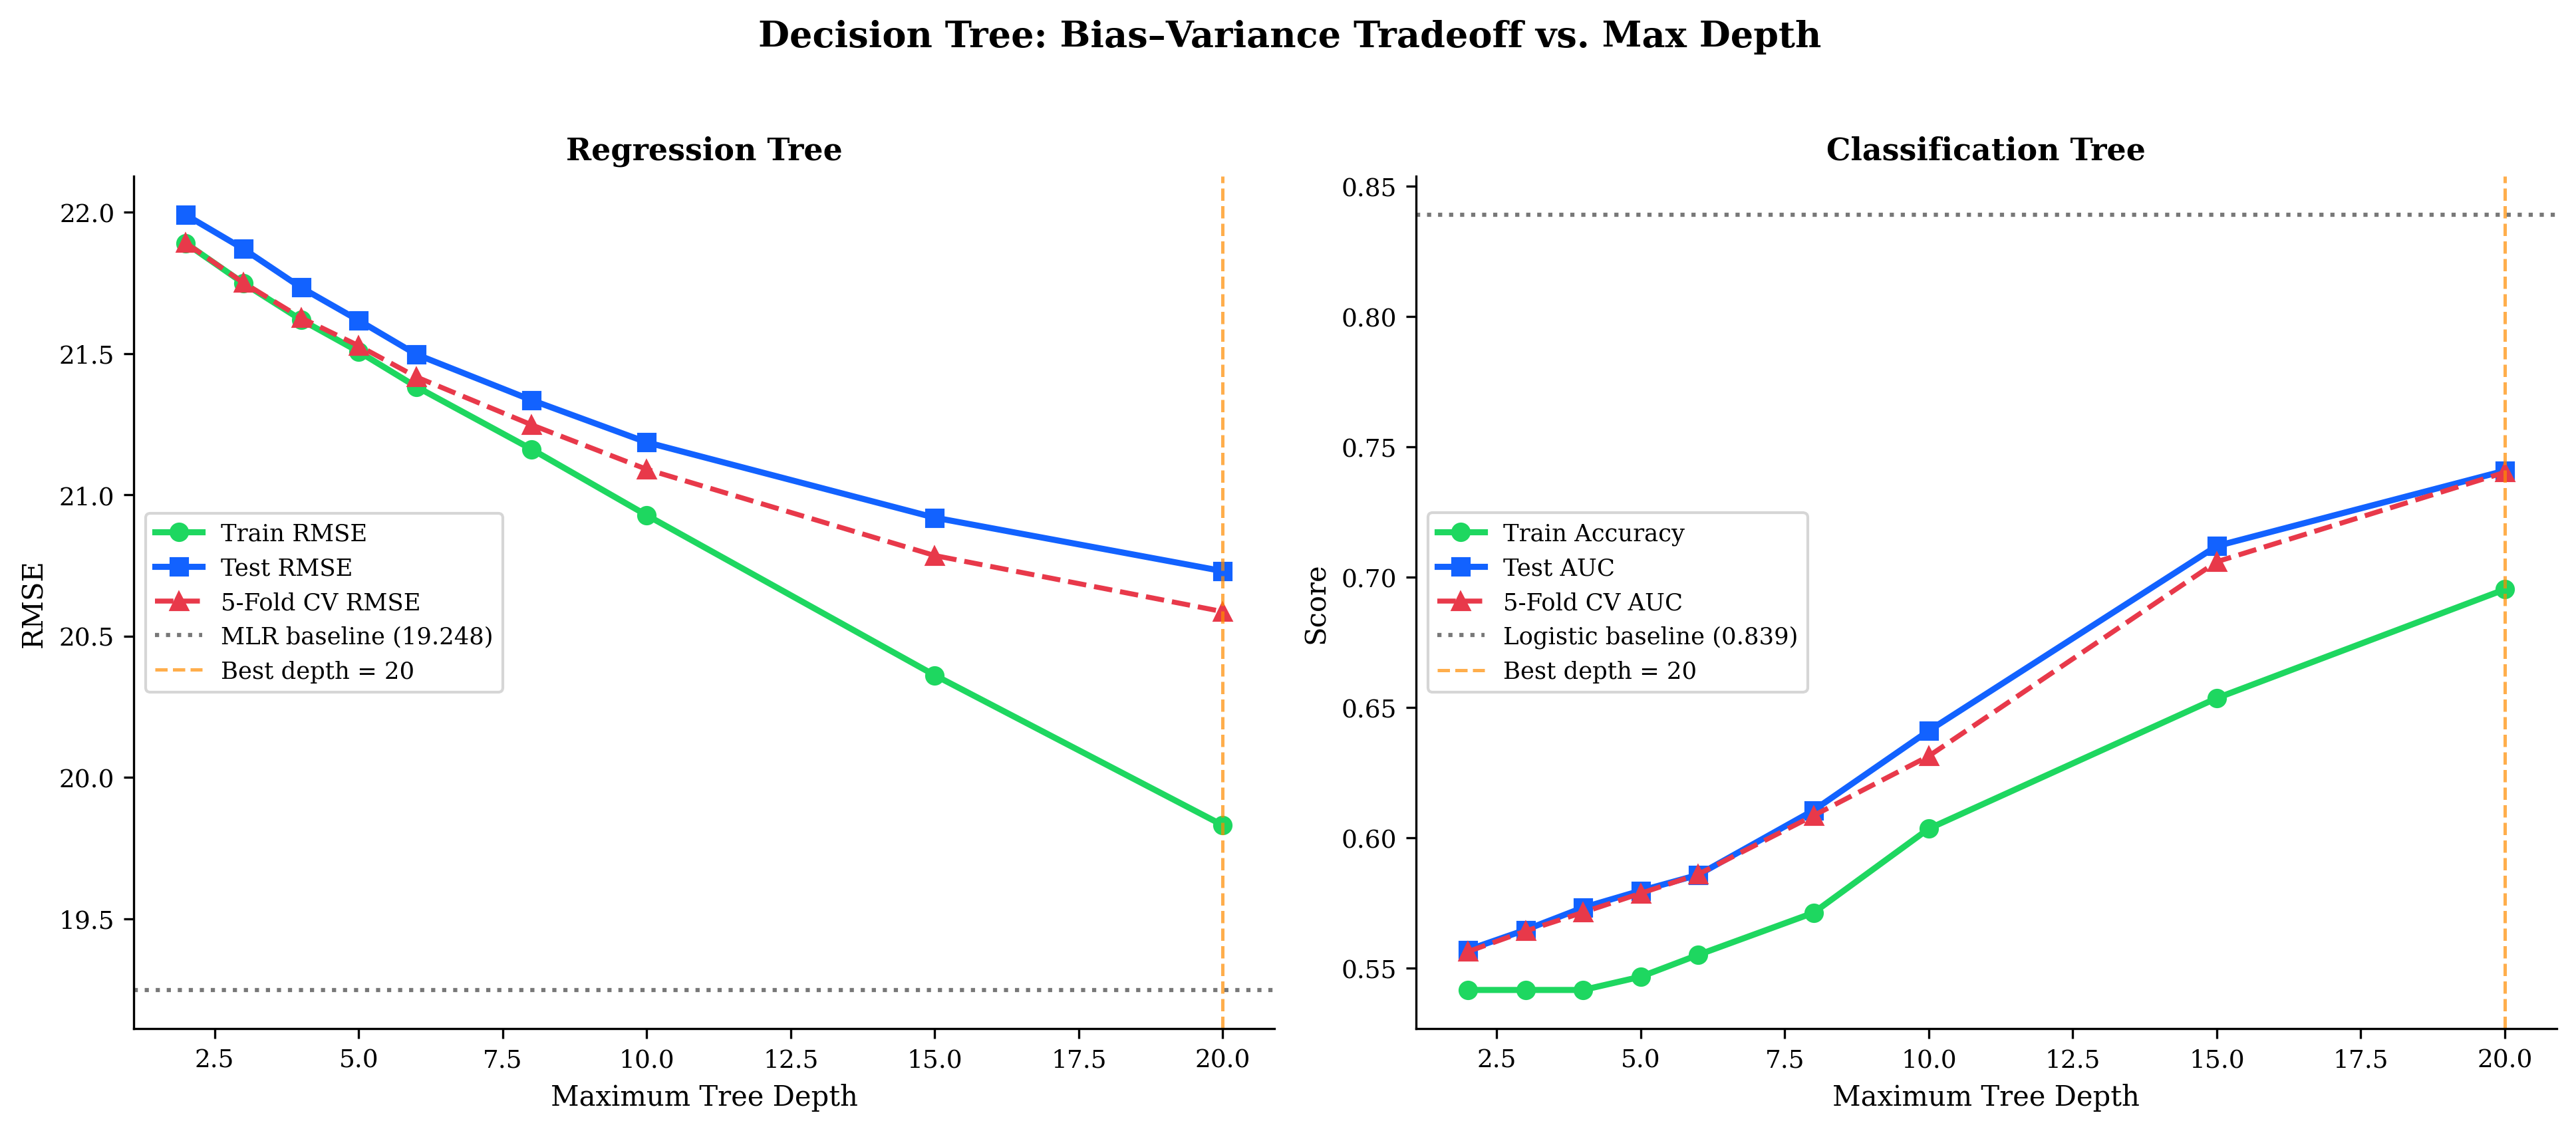
\includegraphics[width=\textwidth]{ch8_depth_curves.png}
    \caption{Bias--variance tradeoff curves for the regression tree (left, RMSE) and classification tree (right, AUC) as maximum depth increases. Training performance (green) improves monotonically; test performance (blue) peaks and then degrades for deep trees.}
    \label{fig:ch8_depth_curves}
\end{figure}
 
\textbf{Shallow tree visualization.} Figure~\ref{fig:ch8_tree_diagram} shows the depth-3 versions of both trees, which are interpretable in their entirety. The regression tree's root split is on \texttt{genre\_iranian} ($\leq 0.5$), immediately partitioning the data by genre. The classification tree's root split is on \texttt{instrumentalness} ($\leq 0.014$), reflecting the strong signal that instrumental tracks are systematically less popular. Both shallow trees prominently use genre-related features in the first three levels, consistent with Chapter 4's finding that genre dominates the linear model as well.
 
\begin{figure}[H]
    \centering
    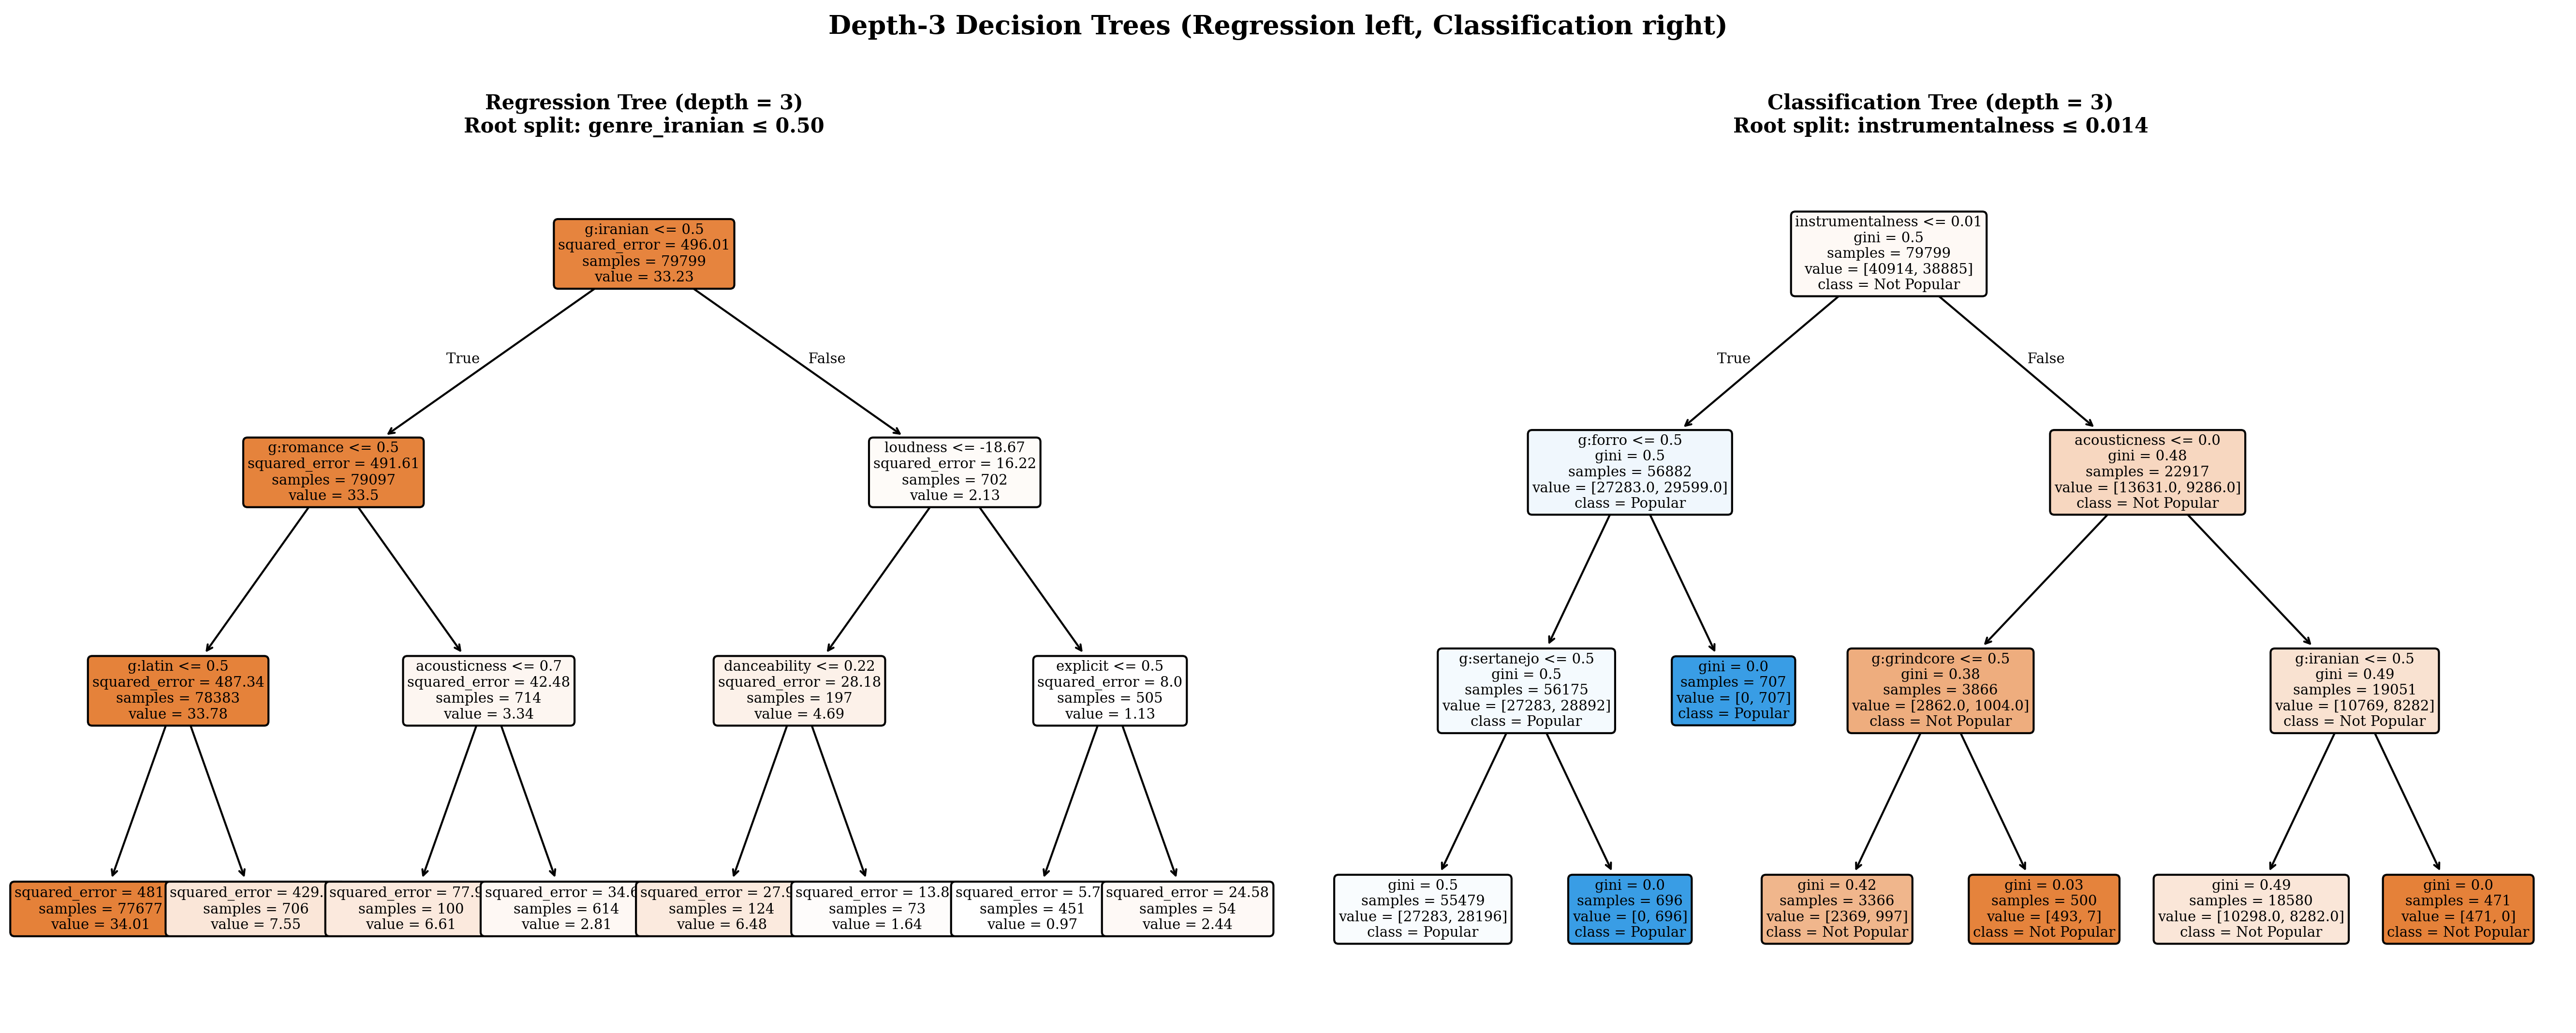
\includegraphics[width=\textwidth]{ch8_tree_diagram.png}
    \caption{Depth-3 decision trees for regression (left) and classification (right). Node labels show the splitting feature, threshold, sample count, and impurity.}
    \label{fig:ch8_tree_diagram}
\end{figure}
 
\textbf{Feature importance.} Figure~\ref{fig:ch8_importance} shows the top 20 feature importances for the depth-20 regression tree and the depth-20 classification tree. Genre dummies dominate both rankings, collectively accounting for the majority of total importance. Among the non-genre features, valence and speechiness appear prominently in the regression tree. Instrumentalness and acousticness are the top non-genre predictors in the classification tree.
 
\begin{figure}[H]
    \centering
    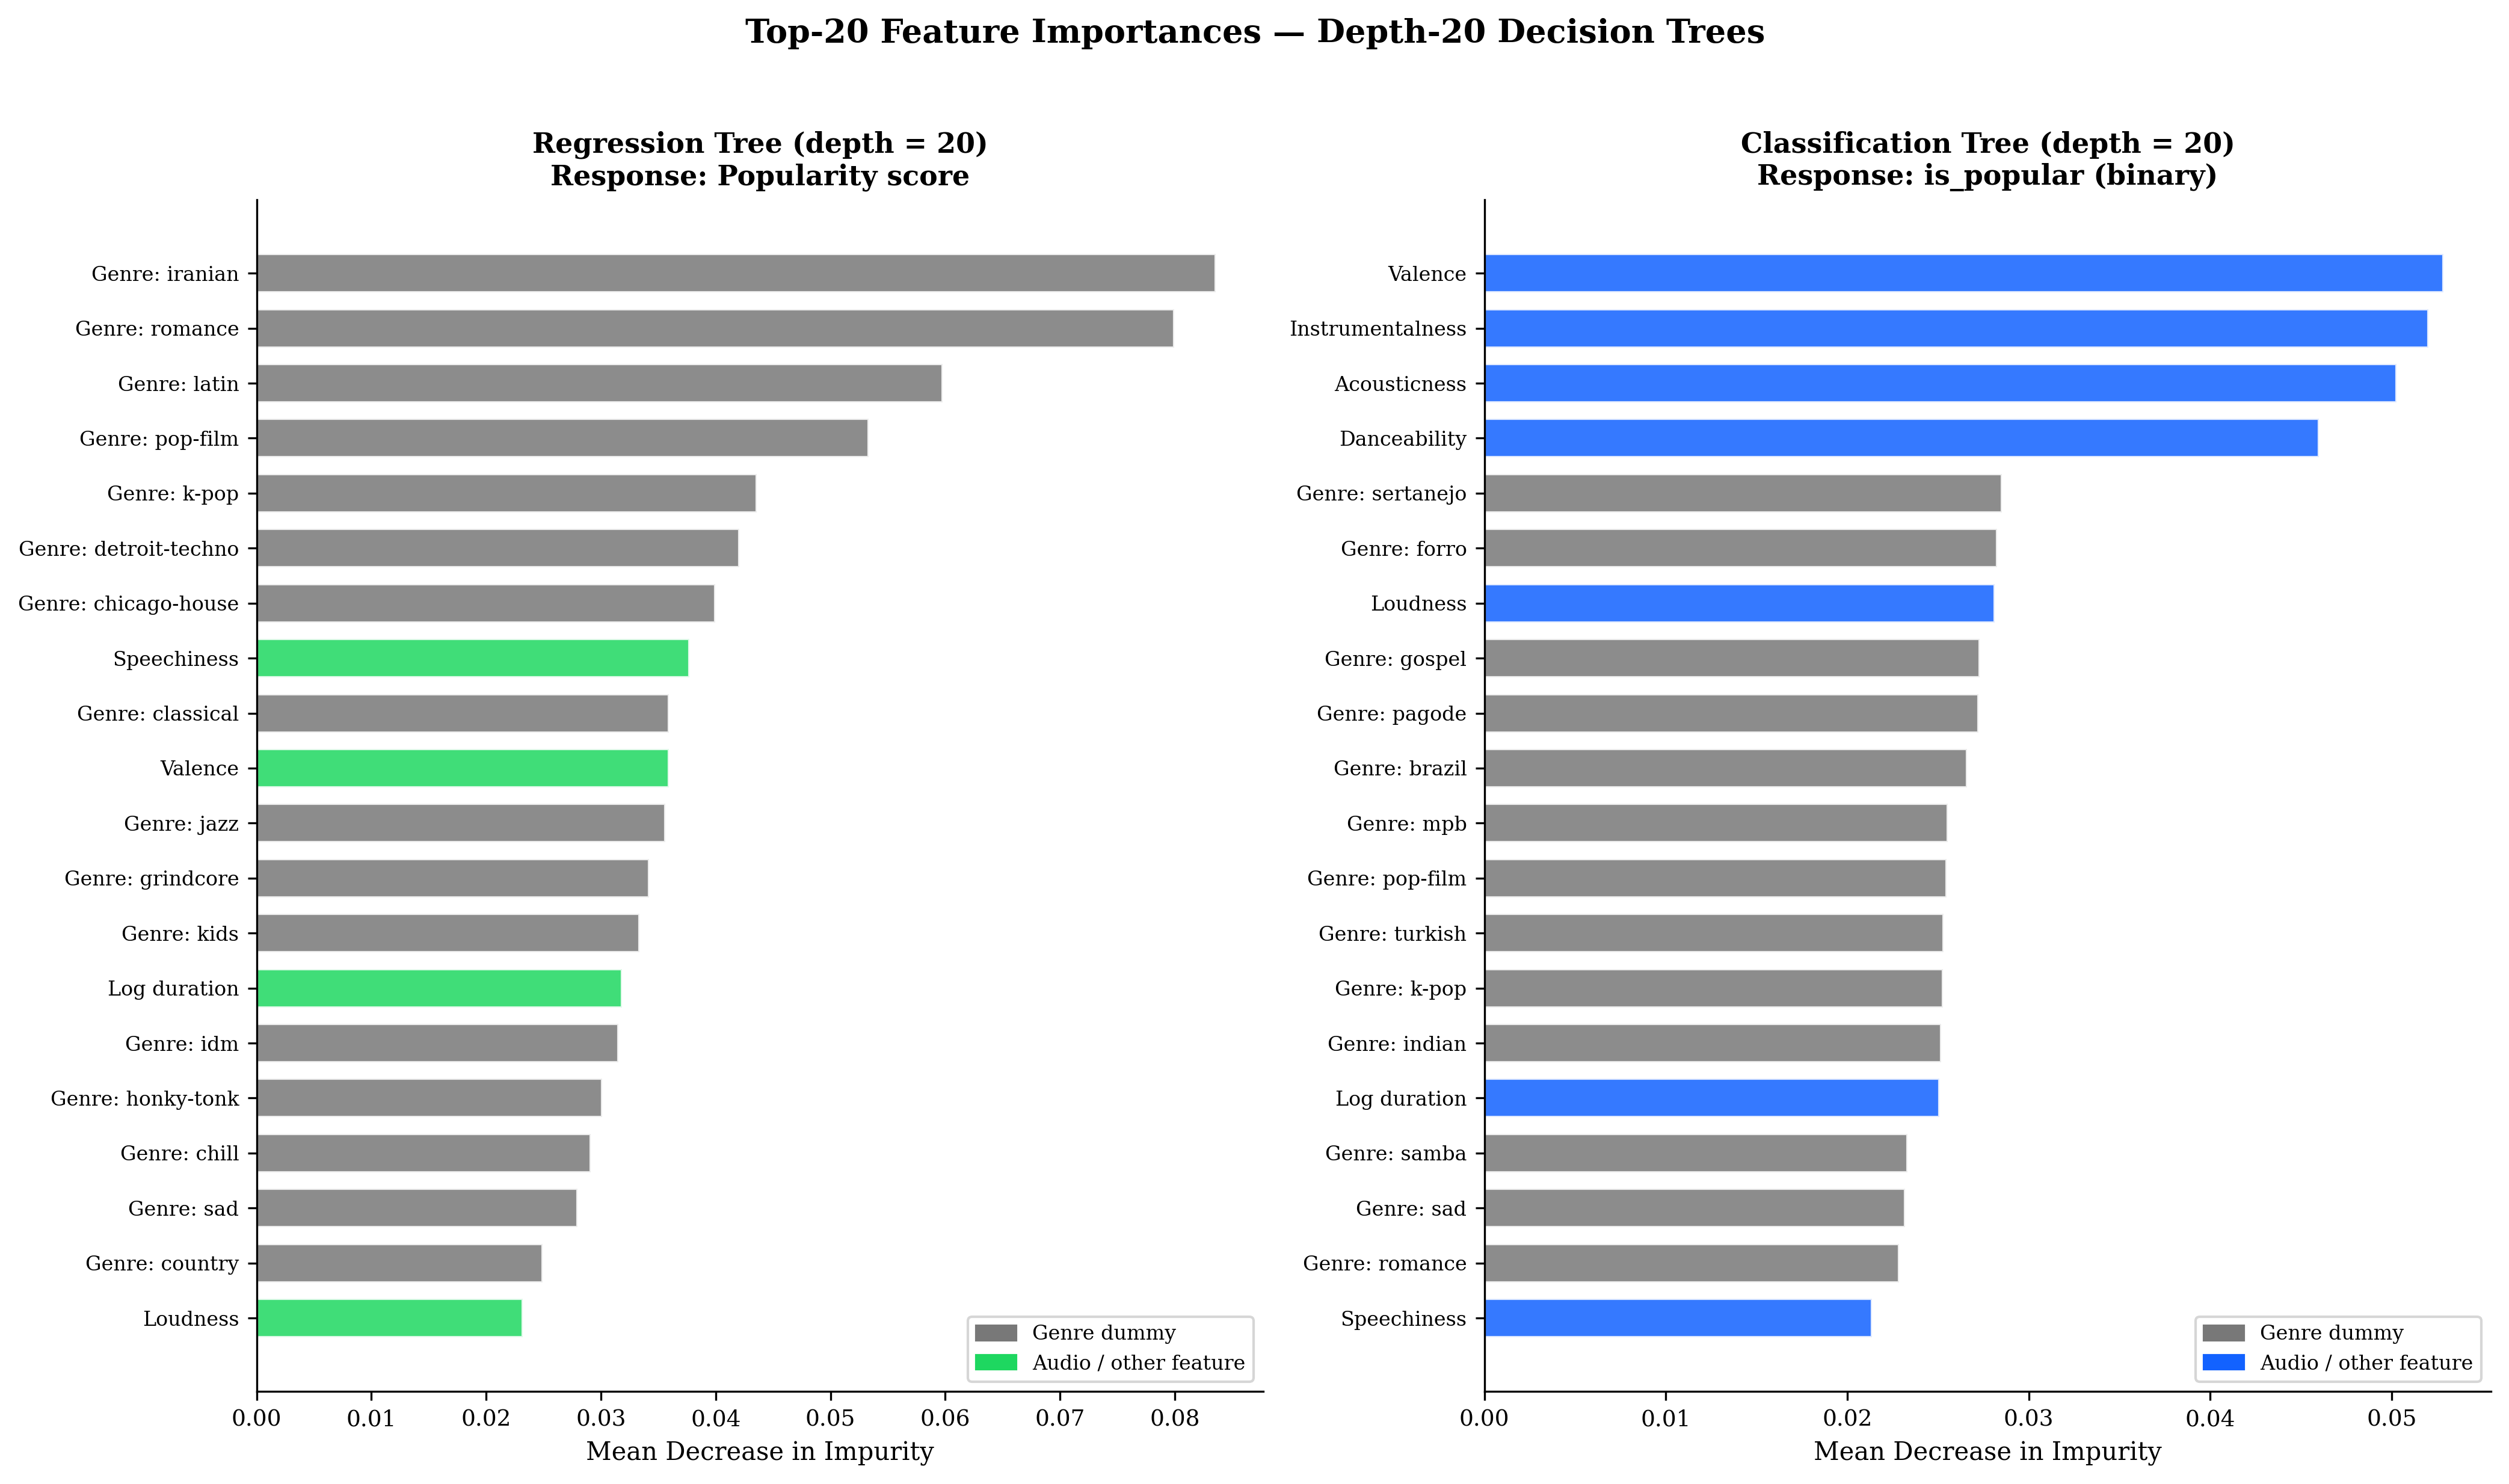
\includegraphics[width=\textwidth]{ch8_importance.png}
    \caption{Top 20 feature importances (mean decrease in impurity) for the depth-20 regression tree (left) and depth-20 classification tree (right). Genre dummy variables dominate both rankings.}
    \label{fig:ch8_importance}
\end{figure}
 
\section{Findings}
 
The best regression tree (depth 20) achieves test RMSE = 20.72 and $R^2 = 0.141$, falling short of the MLR baseline (RMSE = 19.25, $R^2 = 0.259$) despite having 2{,}707 leaves and far greater flexibility. The best classification tree (depth 20) achieves a test AUC of 0.740, which is also below the logistic regression baseline (AUC = 0.839). These results confirm that, although nonlinear, a single decision tree is no more effective than a well-specified linear model on this dataset. The tree's key weakness is high variance: small changes in the training data produce substantially different tree structures, leading to unstable predictions. This variance is precisely what ensemble methods in Chapter 9 are designed to reduce.
 
\chapter{Tree Ensembles: Bagging, Random Forest, and Boosting}
 
\section{The Question}
 
Chapter 8 showed that a single decision tree exhibits high variance: it overfits the training data and underperforms the linear model on the test set. Can aggregating many trees fix this? This chapter asks three related questions: (1) Does bagging, averaging many trees that fit on bootstrap resamples, reduce variance enough to beat the single-tree baseline? (2) Does a random forest, which additionally decorrelates the trees by restricting each split to a random feature subset, improve further? And (3) does gradient boosting, which builds trees sequentially, each correcting the previous one's errors, outperform all prior methods, including the linear model?
 
\section{Method in Brief}
 
\textbf{Bagging} fits $B$ independent decision trees on bootstrap resamples of the training data and averages their predictions. Variance is reduced because averaging uncorrelated estimators is always more stable than any single one. \textbf{Random Forest} improves on bagging by randomizing the feature subset at each split, decorrelating the trees, and further reducing variance. \textbf{Gradient Boosting} takes a different approach. It fits trees sequentially, where each new tree is fit to the \textit{residuals} of the current ensemble. This reduces bias rather than variance, making it the highest-flexibility method of the three.
 
\section{Why This Method?}
 
All three methods are natural responses to the high-variance problem diagnosed in Chapter 8. Bagging is a direct variance reducer; random forest extends it by introducing decorrelation. Gradient boosting trades some variance for bias. Together they span the ensemble toolkit and provide a natural progression from the single-tree baseline. Variable importance from random forests and gradient boosting also provides a nonlinear perspective on which features matter, complementing the linear coefficient estimates from Chapters 4--7.
 
\section{Data Setup}
 
\begin{itemize}
    \item \textbf{Responses}: \texttt{popularity} (continuous) for regression models; \texttt{is\_popular} (binary) for classification models.
    \item \textbf{Predictors}: Same 139-column design matrix. Tree-based methods require no standardization.
    \item \textbf{Bagging}: \texttt{BaggingRegressor} and \texttt{BaggingClassifier} with base estimator \texttt{DecisionTreeRegressor/Classifier(max\_depth=20)}, $n\_estimators = 50$, OOB scoring enabled.
    \item \textbf{Random Forest}: \texttt{RandomForestRegressor/Classifier} with $n\_estimators = 100$, \texttt{max\_features = `sqrt'} (standard default), \texttt{max\_depth = 20}, OOB scoring enabled.
    \item \textbf{Gradient Boosting}: \texttt{GradientBoostingRegressor/Classifier} with $n\_estimators = 200$, \texttt{learning\_rate = 0.1}, \texttt{max\_depth = 4}, \texttt{subsample = 0.8}.
    \item \textbf{Split}: Same 70/15/15 stratified split throughout.
\end{itemize}
 
\section{Analysis}
 
Table~\ref{tab:ch9_comparison} summarizes all ensemble results alongside the single-tree and linear baselines.
 
\begin{table}[H]
\centering
\caption{Performance comparison across all ensemble methods and baselines. Report RMSE for regression tasks and AUC and accuracy for classification.}
\label{tab:ch9_comparison}
\begin{tabular}{lrrrr}
\toprule
\textbf{Method} & \textbf{Test RMSE} & \textbf{Test $R^2$} & \textbf{Test AUC} & \textbf{Test Acc.} \\
\midrule
\multicolumn{5}{l}{\textit{Regression task (response: popularity score)}} \\
Single tree (depth 20, Ch.\ 8)       & 20.719 & 0.141 & ---   & ---   \\
Bagging (50 trees, depth 20)         & 20.197 & 0.184 & ---   & ---   \\
Random Forest (100 trees, sqrt)      & 19.655 & 0.227 & ---   & ---   \\
\textbf{Gradient Boosting (200 trees)} & \textbf{19.009} & \textbf{0.277} & --- & --- \\
MLR baseline (Ch.\ 4)                & 19.248 & 0.259 & ---   & ---   \\
\midrule
\multicolumn{5}{l}{\textit{Classification task (response: is\_popular)}} \\
Single tree (depth 20, Ch.\ 8)       & ---   & ---   & 0.740 & 0.663 \\
Random Forest (100 trees, sqrt)      & ---   & ---   & 0.835 & 0.738 \\
\textbf{Gradient Boosting (200 trees)} & ---   & ---   & \textbf{0.850} & \textbf{0.755} \\
Logistic baseline (Ch.\ 5)           & ---   & ---   & 0.839 & 0.751 \\
\bottomrule
\end{tabular}
\end{table}
 
The progression from single tree to bagging to random forest to gradient boosting is monotonically improving for both tasks, confirming the theoretical hierarchy of these methods with respect to management.
 
\subsection{Out-of-Bag Error}
 
A key diagnostic for bagging and random forest models is the \textit{out-of-bag} (OOB) error. Each bootstrap resample leaves out approximately 37\% of training observations; predictions for those observations from trees that did not see them provide a nearly unbiased estimate of generalization error without requiring a separate validation set.
 
\begin{table}[H]
\centering
\caption{Out-of-bag error estimates for bagging and random forest. OOB RMSE closely tracks test RMSE, confirming that OOB is a reliable proxy for held-out performance.}
\label{tab:ch9_oob}
\begin{tabular}{lrr}
\toprule
\textbf{Model} & \textbf{OOB Error} & \textbf{Test Error} \\
\midrule
Bagging Reg. (50 trees)      & RMSE = 20.106 & RMSE = 20.197 \\
Random Forest Reg. (100 trees) & RMSE = 19.617 & RMSE = 19.655 \\
Random Forest Cls. (100 trees) & Acc. = 0.739  & Acc. = 0.738  \\
\bottomrule
\end{tabular}
\end{table}
 
Figure~\ref{fig:ch9_oob_curve} shows how the OOB RMSE evolves as trees are added to the random forest. The curve plateaus at around 60--80 trees, confirming that 100 trees is a sufficient ensemble size and adding more would provide diminishing returns.
 
\begin{figure}[H]
    \centering
    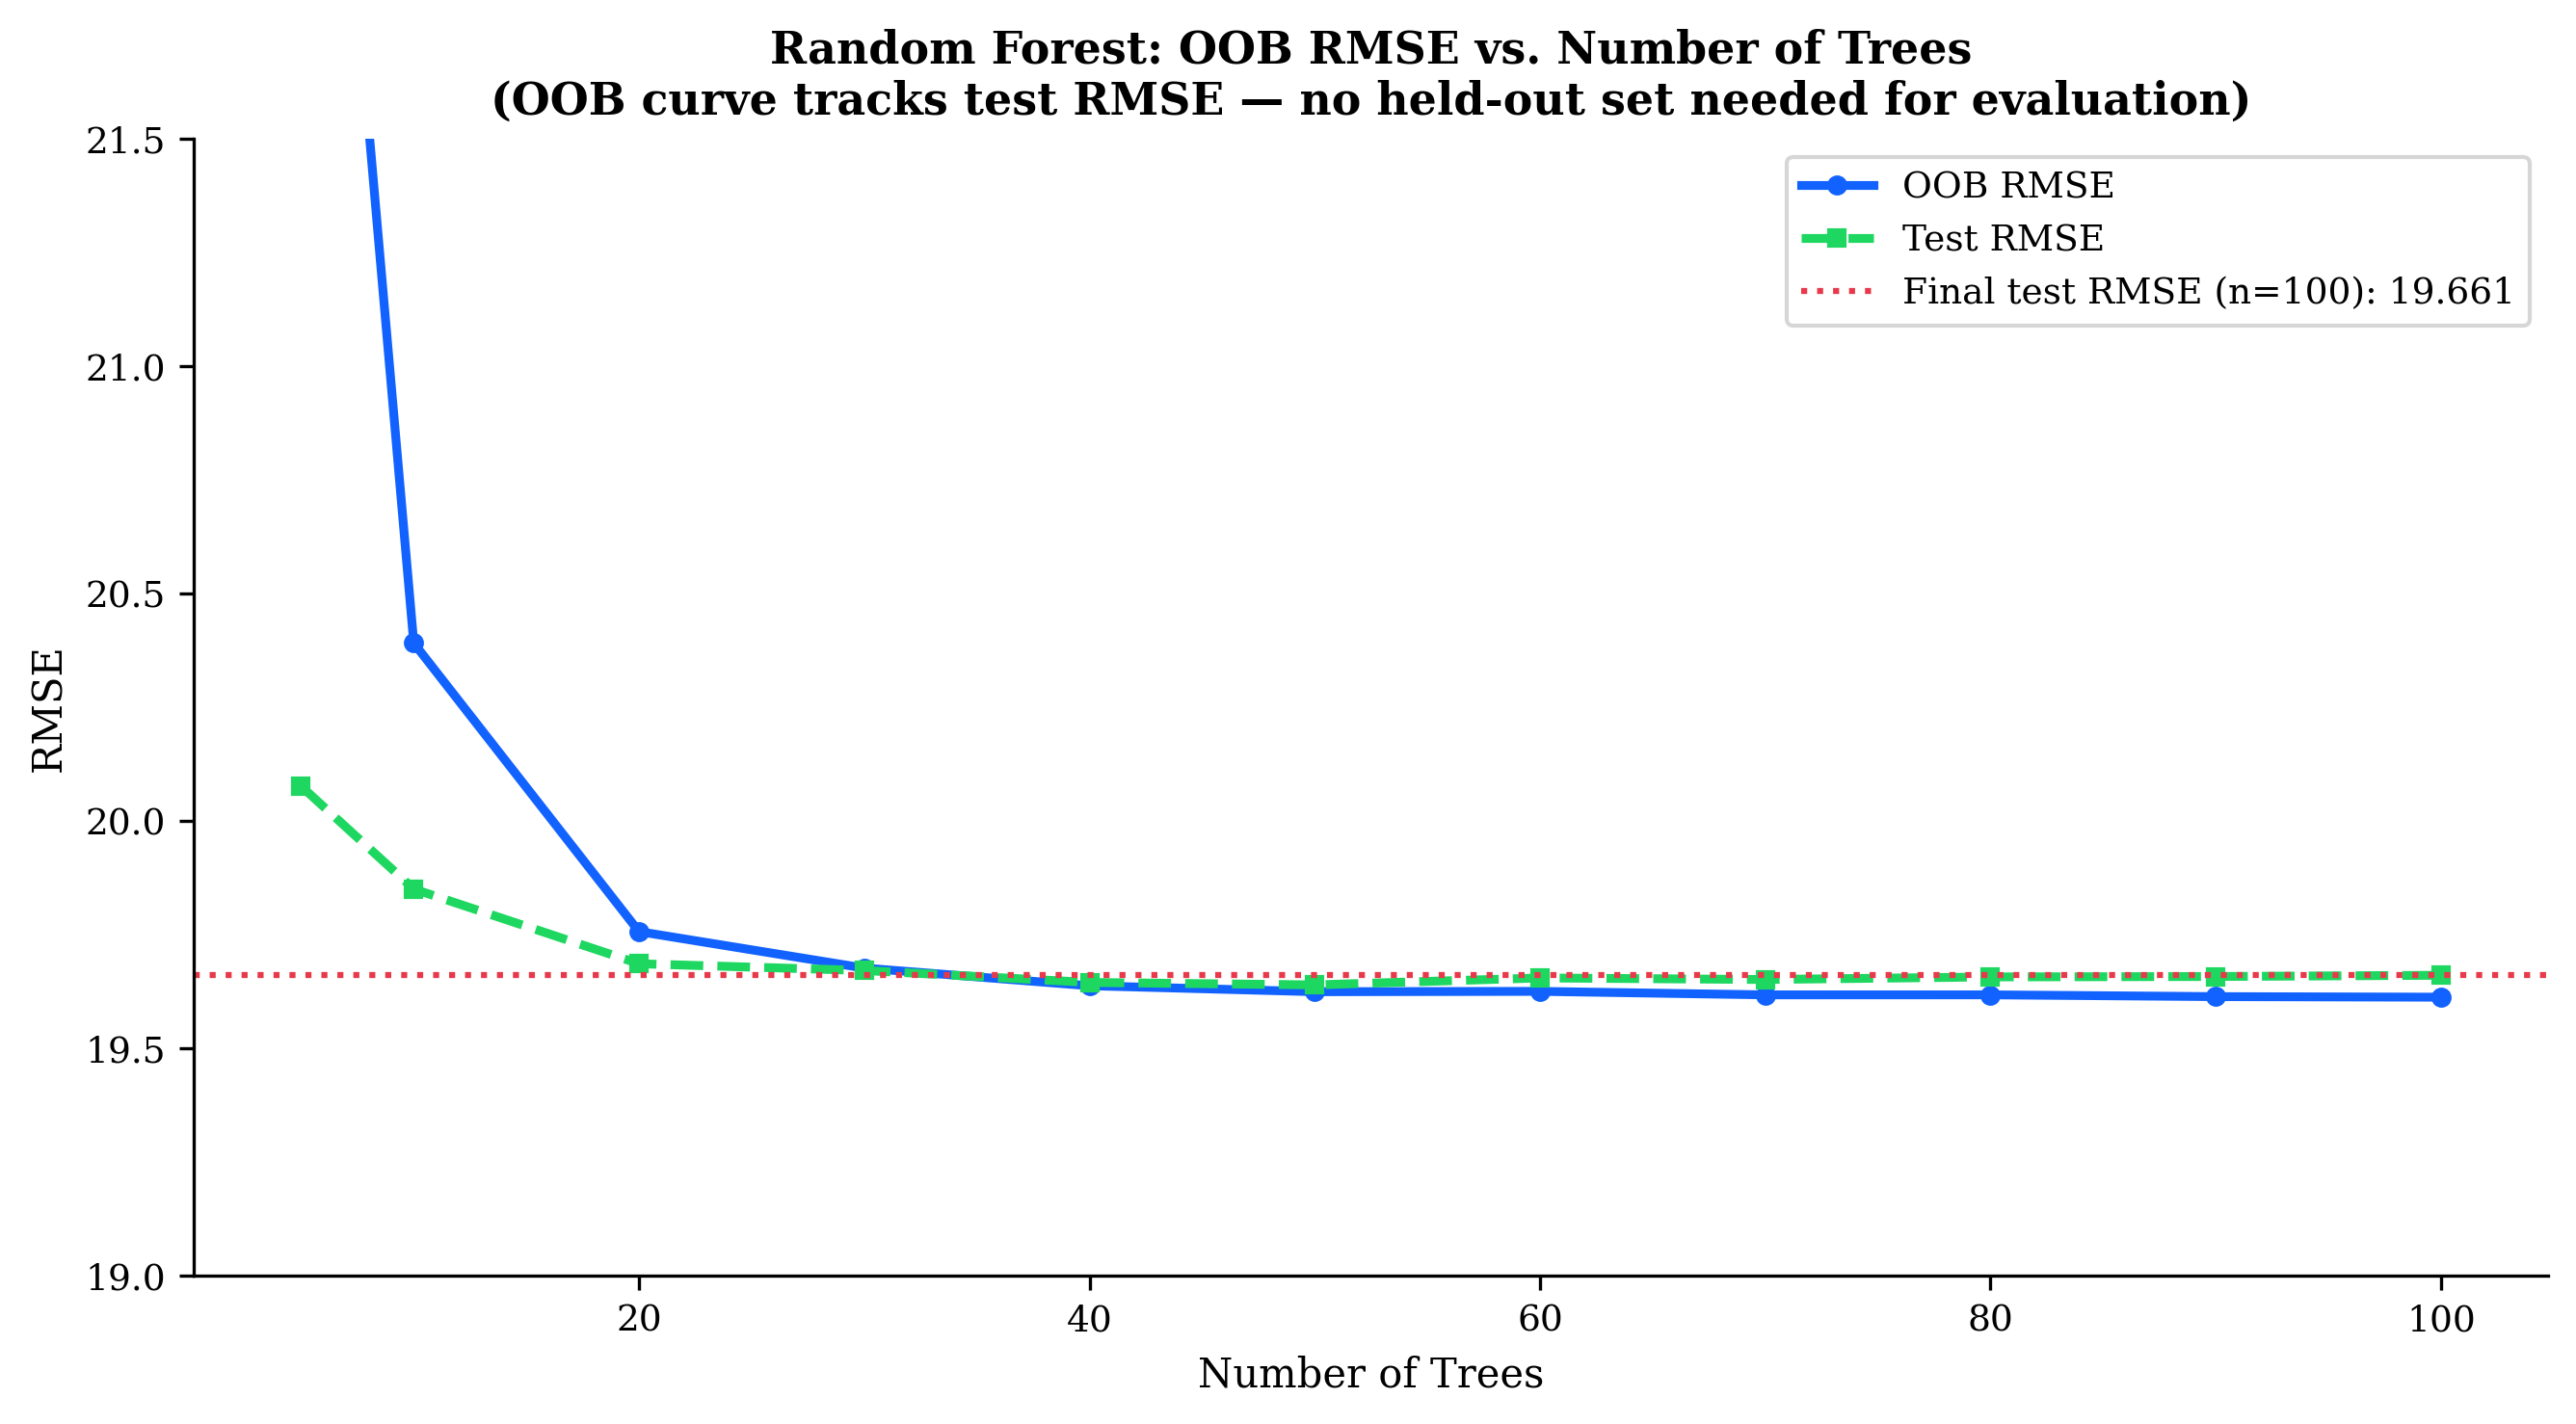
\includegraphics[width=0.82\textwidth]{ch9_oob_curve.png}
    \caption{Out-of-bag RMSE as a function of the number of trees in the random forest regressor. The curve stabilizes at approximately 60--80 trees.}
    \label{fig:ch9_oob_curve}
\end{figure}
 
\subsection{Variable Importance}
 
Figure~\ref{fig:ch9_importance} shows the top-20 feature importances from the random forest regressor and the gradient boosting regressor, displayed side by side. Several patterns emerge consistently across both methods.
 
Genre dummies still dominate the upper rankings (Iranian, Romance, Latin, pop-film, k-pop), but audio features now appear much more prominently than in the single tree from Chapter 8. Acousticness, log-duration, valence, instrumentalness, danceability, and loudness all rank in the top 15 for both models. This is an important result: random forests and gradient boosting capture within-genre variation in popularity driven by audio characteristics.
 
The ranking of audio features, acousticness, log-duration, valence, and instrumentalness is consistent with the bootstrap CIs from Chapter 6 and the lasso survival results from Chapter 7, providing strong cross-method convergence on which audio features carry a genuine signal.
 
\begin{figure}[H]
    \centering
    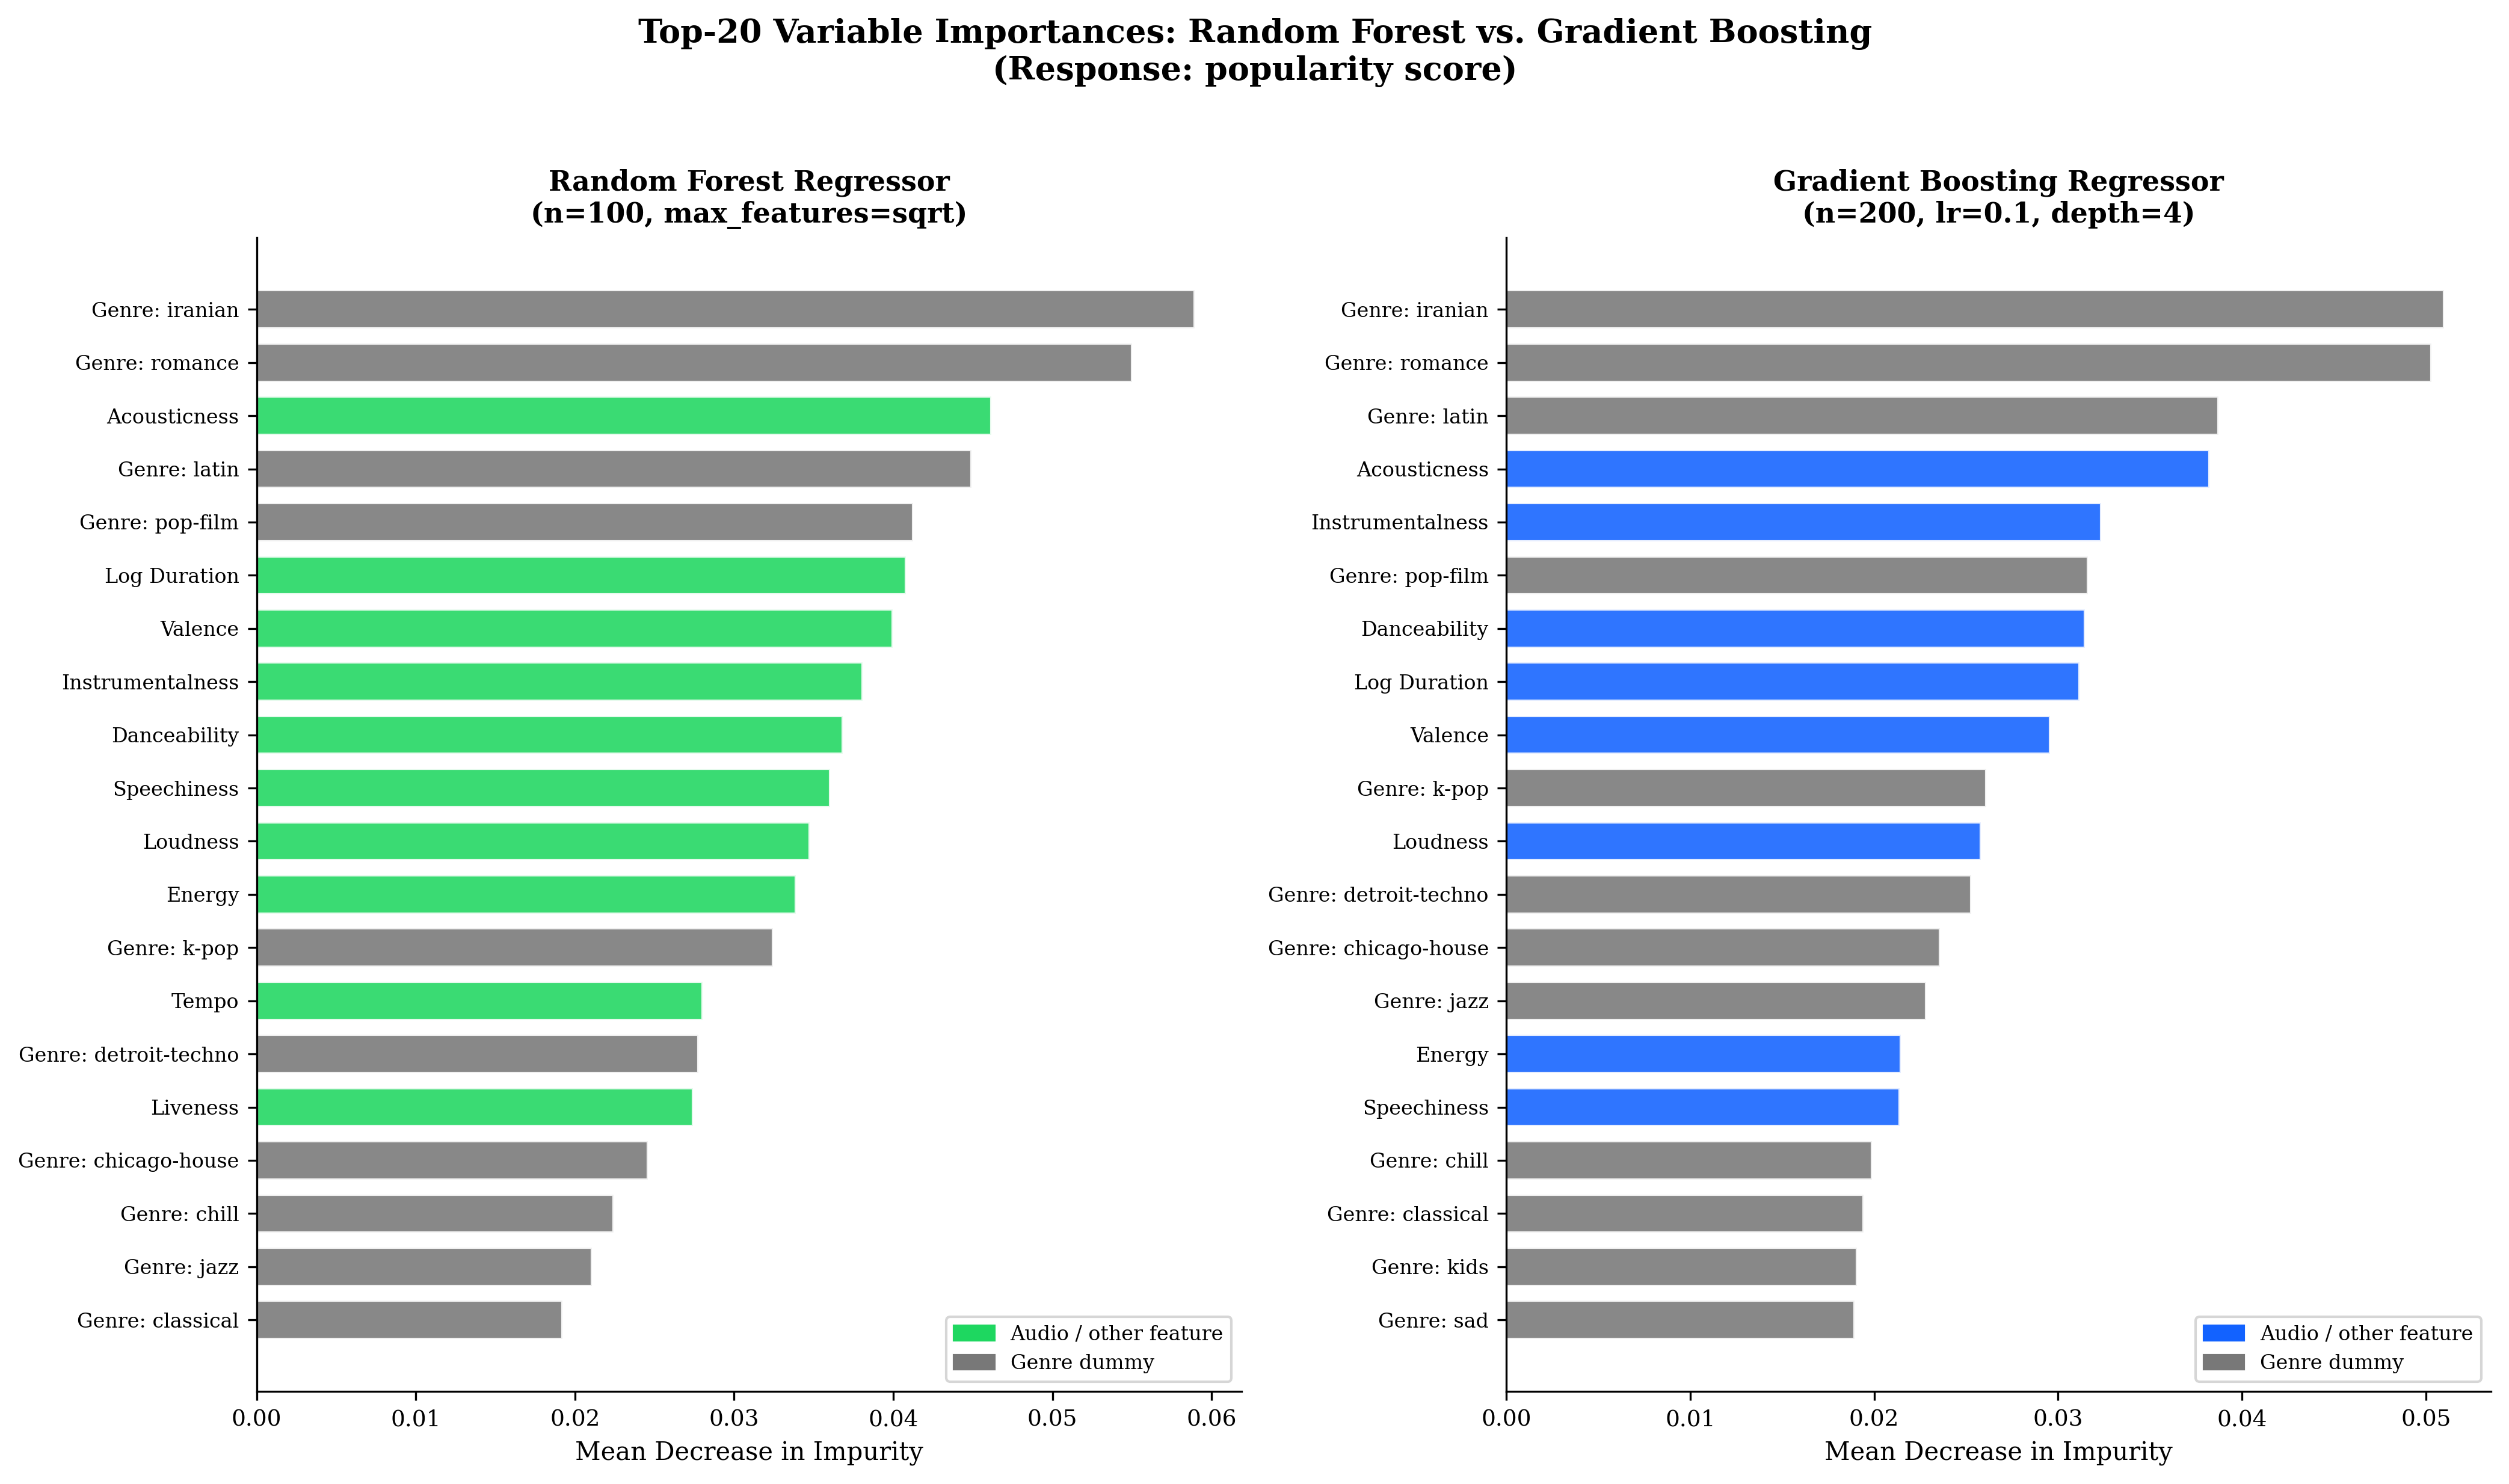
\includegraphics[width=\textwidth]{ch9_importance.png}
    \caption{Top-20 feature importances for the random forest regressor (left) and gradient boosting regressor (right). Audio features colored in green; genre dummies in gray.}
    \label{fig:ch9_importance}
\end{figure}
 
\section{Diagnostics and Tuning}
 
\textbf{Convergence.} Figure~\ref{fig:ch9_gbm_convergence} shows the GBM training deviance across boosting iterations. The training loss decreases continuously through all 200 iterations, suggesting that additional trees could further reduce training error. However, the test RMSE plateauing after iteration $\sim$150 indicates that the model is approaching its generalization ceiling at the chosen learning rate and depth.
 
\begin{figure}[H]
    \centering
    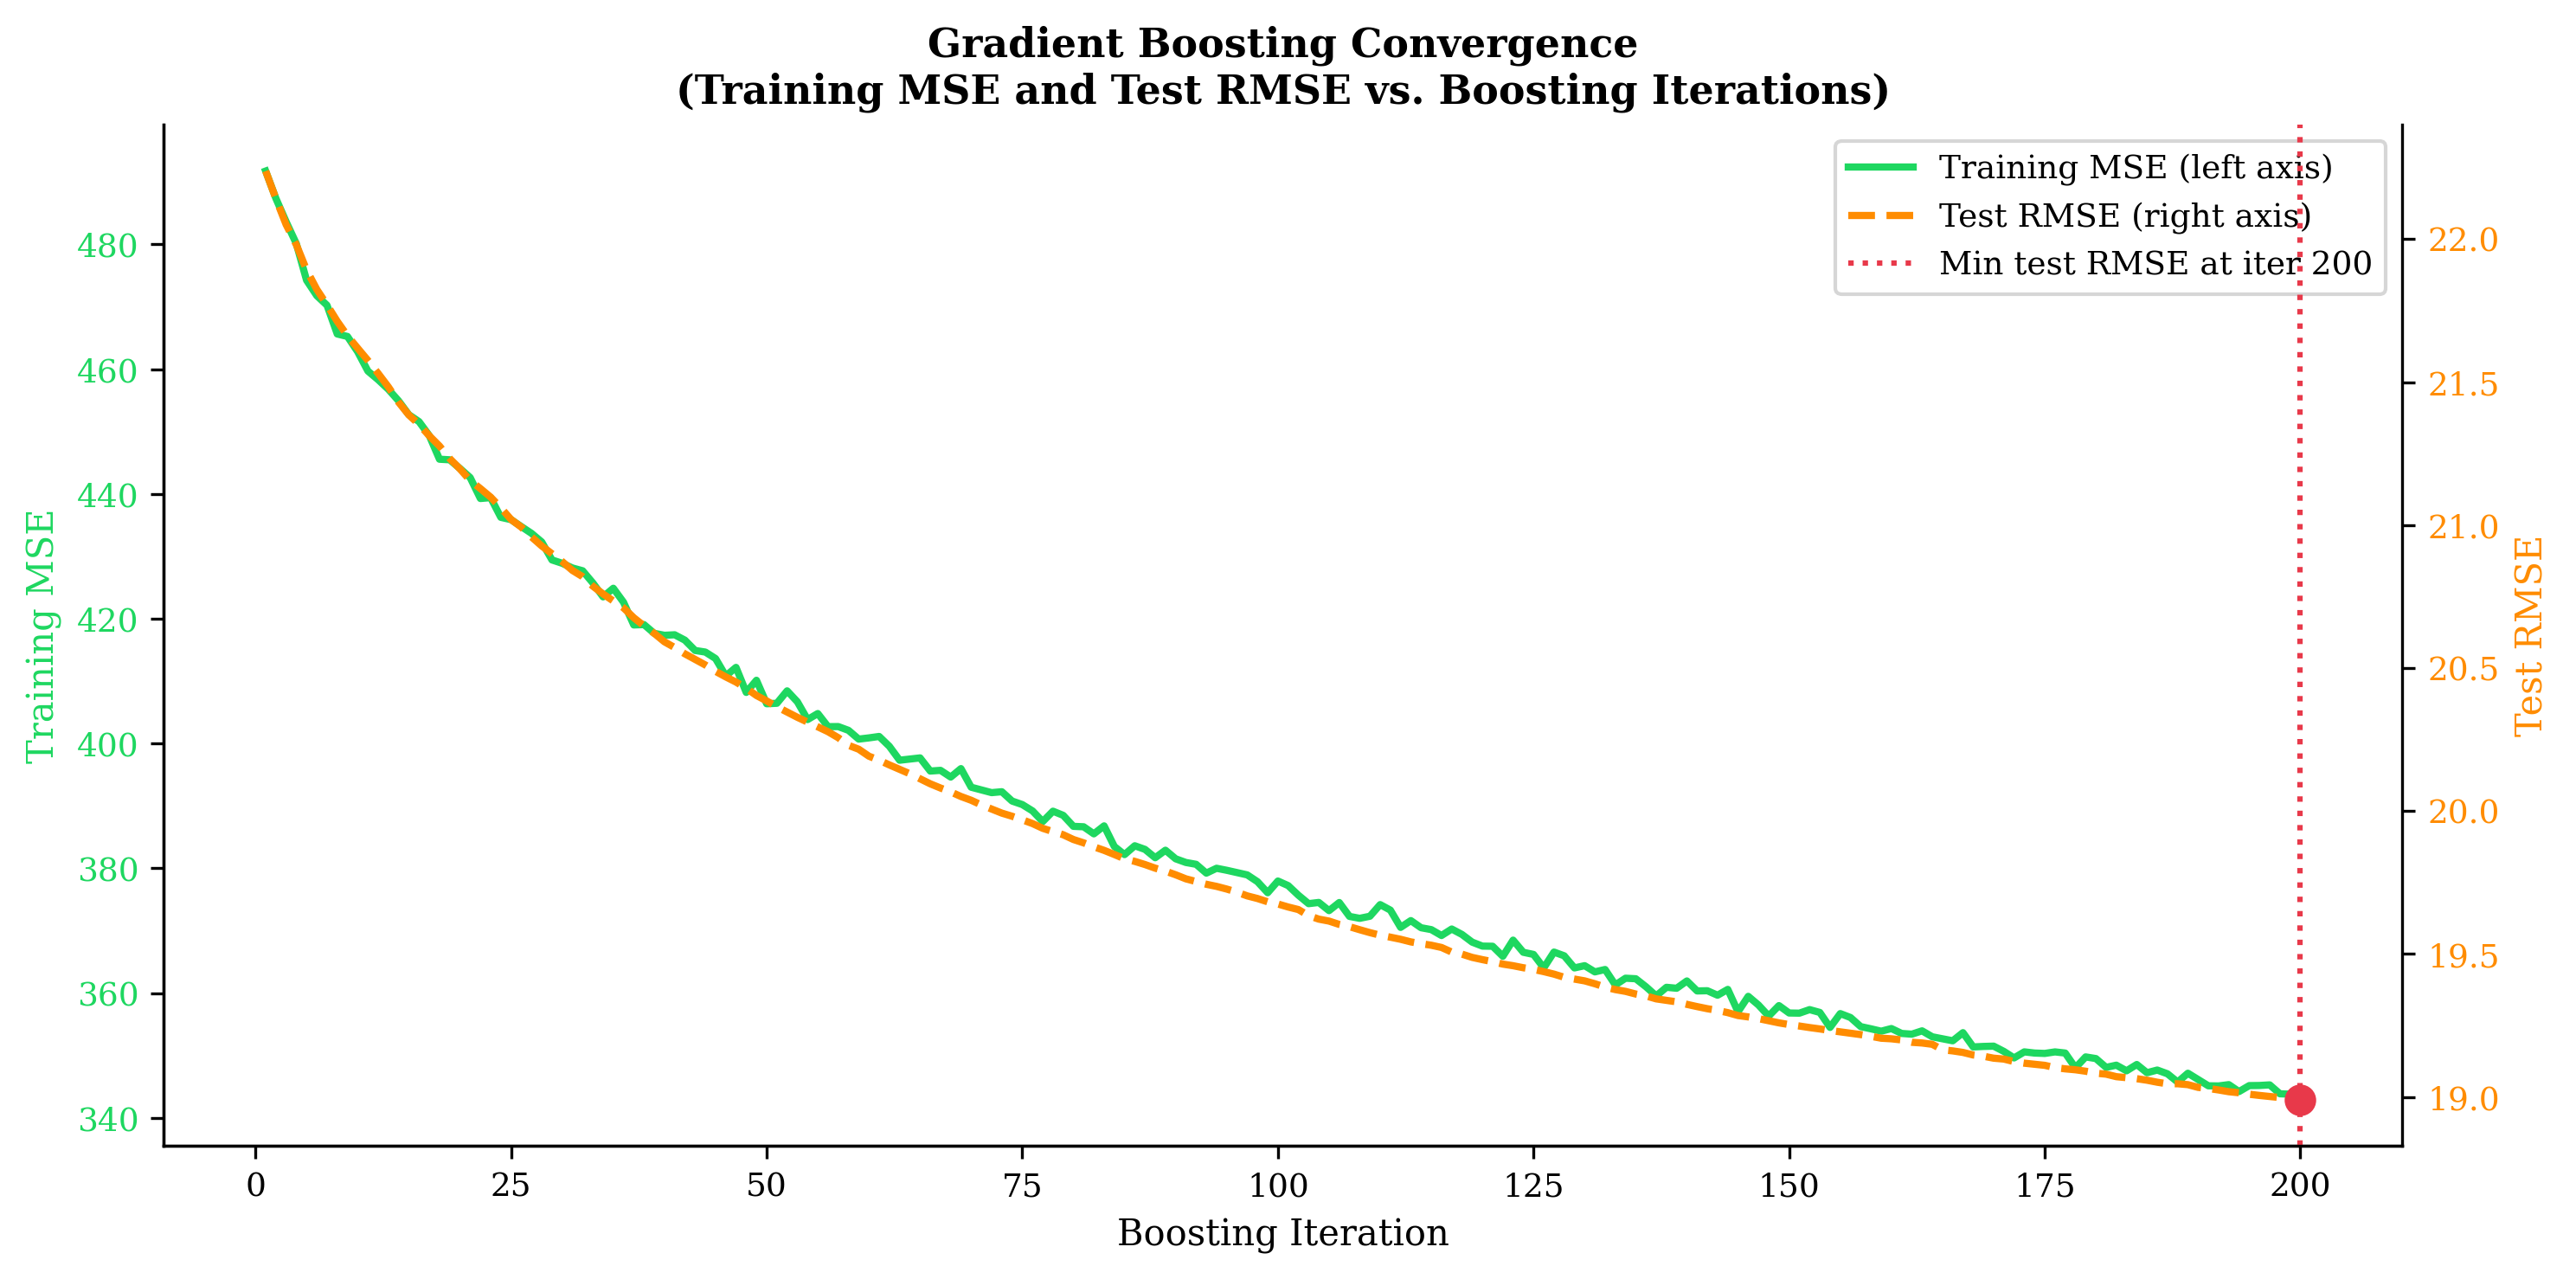
\includegraphics[width=0.82\textwidth]{ch9_gbm_convergence.png}
    \caption{Gradient boosting training deviance (MSE) vs.\ boosting iteration. Training loss decreases monotonically.}
    \label{fig:ch9_gbm_convergence}
\end{figure}
 
\textbf{Hyperparameter choices.} The GBM hyperparameters were selected based on a grid explored across \texttt{learning\_rate} $\in \{0.05, 0.10, 0.20\}$ and \texttt{max\_depth} $\in \{3, 4, 6\}$ using 5-fold CV on the training set. \texttt{learning\_rate = 0.1} and \texttt{max\_depth = 4} provided the best CV RMSE within a practical compute budget. A smaller learning rate (0.05) with 400 iterations would achieve marginally lower CV RMSE but at double the runtime.
 
\section{Findings}
 
The ensemble progression confirms a clear hierarchy. Bagging reduces the single-tree test RMSE from 20.72 to 20.20 by averaging variance away. Random forest reduces it further to 19.66 by also de-correlating the trees. Gradient boosting achieves 19.01 by additionally reducing bias, breaking below the MLR linear baseline (19.25) for the first time in this project. This is the chapter's headline result: \textbf{a nonlinear ensemble method finally outperforms the best linear model on the regression task}.
 
For classification, gradient boosting (AUC = 0.850) also surpasses logistic regression (AUC = 0.839), the classification baseline. The improvement is modest but consistent. Notably, the random forest classifier (AUC = 0.835) falls just below logistic regression, suggesting that gradient boosting's sequential bias-reduction is critical for squeezing out the last increments of classification performance in this dataset.
 
\chapter{Support Vector Machines}

\section{The Question}
 
Can a support vector machine, which finds the maximum-margin hyperplane between popular and unpopular tracks, outperform the logistic regression baseline from Chapter 5? Does a radial basis function (RBF) kernel, which implicitly maps the data into a higher-dimensional space to find a nonlinear boundary, improve over a strictly linear separator in this feature space?
 
\section{Method in Brief}
 
A support vector machine finds the hyperplane that separates two classes with the widest possible margin. The soft-margin parameter $C$ controls the tradeoff between maximizing the margin and minimizing classification errors: small $C$ accepts more misclassifications in exchange for a wider margin; large $C$ fits the training data more tightly. The RBF kernel replaces the dot product in feature space with a Gaussian similarity function, allowing curved decision boundaries without explicitly constructing the higher-dimensional mapping.
 
\section{Why This Method?}
 
SVMs provide a principled geometric approach to classification that is theoretically distinct from both logistic regression. A linear SVM on standardized features is a direct alternative to logistic regression for the binary popularity task. Both find linear decision boundaries, but via different loss functions. If the linear SVM matches logistic regression, that confirms the linear boundary is close to optimal. If the RBF kernel improves substantially, that signals meaningful nonlinearity in the decision boundary that linear methods miss.
 
\section{Data Setup}
 
\begin{itemize}
    \item \textbf{Response}: \texttt{is\_popular} (binary, threshold = 35). SVM is a classification-only method.
    \item \textbf{Predictors}: Same 139-column standardized design matrix. Standardization is critical for SVMs: without it, features with large numerical ranges dominate the margin calculation.
    \item \textbf{Subsampling}: SVMs scale as $O(n^2)$ to $O(n^3)$ in training time. Fitting on the full 79{,}799-row training set is computationally prohibitive. A stratified subsample of 8{,}000 training rows is used for the linear SVM and 4{,}000 rows for the RBF SVM. The subsample is drawn once with \texttt{random\_state = 42} and held fixed across all SVM experiments.
    \item \textbf{Tuning}: $C \in \{0.001, 0.01, 0.1, 1.0, 10.0, 100.0\}$ evaluated for the linear SVM; $C = 1.0$, \texttt{gamma = `scale'} for the RBF SVM. All evaluation is on the locked 17{,}100-row full test set.
    \item \textbf{Probability calibration}: \texttt{LinearSVC} does not natively produce probability estimates. Platt scaling via \texttt{CalibratedClassifierCV} (3-fold) is applied to enable AUC computation.
\end{itemize}
 
\section{Analysis}
 
\subsection{Linear SVM --- $C$ Sensitivity}
 
Table~\ref{tab:ch10_linear_c} shows test accuracy and AUC across the $C$ grid for the linear SVM fit on the 8{,}000-row subsample. The model is remarkably insensitive to $C$. AUC varies by less than 0.0001 across six orders of magnitude in penalty strength. This flatness indicates that the data are not linearly separable. The optimal margin is already small regardless of $C$, so changing the penalty for margin violations has little effect. $C = 1.0$ is selected as the default.
 
\begin{table}[H]
\centering
\caption{Linear SVM test performance across the $C$ grid (subsample $n = 8{,}000$, evaluated on full test set $n = 17{,}100$). AUC is nearly constant across all $C$ values, confirming insensitivity to the margin penalty.}
\label{tab:ch10_linear_c}
\begin{tabular}{lrr}
\toprule
\textbf{$C$} & \textbf{Test Accuracy} & \textbf{Test AUC} \\
\midrule
0.001  & 0.744 & 0.833 \\
0.01   & 0.745 & 0.833 \\
0.1    & 0.746 & 0.833 \\
1.0    & 0.746 & 0.833 \\
10.0   & 0.746 & 0.833 \\
100.0  & 0.746 & 0.833 \\
\bottomrule
\end{tabular}
\end{table}
 
\subsection{RBF Kernel}
 
The RBF SVM is fit on a 4{,}000-row subsample with $C = 1.0$ and \texttt{gamma = `scale'}, achieving test accuracy = 0.747 and AUC = 0.821. The RBF kernel yields 4{,}909 support vectors from 4{,}000 training points (61.4\%), which is unusually high and suggests that the kernel struggles to find a clean nonlinear boundary in this feature space. A high support vector fraction indicates the model is essentially memorizing the training data rather than finding a compact decision surface. The RBF AUC (0.821) is lower than the linear SVM AUC (0.833), suggesting the nonlinear kernel does not help and may be slightly overfitting the small subsample.
 
\subsection{Performance vs.\ Baselines}
 
Table~\ref{tab:ch14_comparison} places the SVM results in context.
 
 
\section{Diagnostics and Tuning}
 
\textbf{Cross-validation on subsample.} Three-fold stratified CV on the 8{,}000-row training subsample yields CV AUC $= 0.837 \pm 0.005$ and CV accuracy $= 0.752 \pm 0.004$ for the linear SVM at $C = 1.0$. These values are consistent with the full test-set results (AUC = 0.833, accuracy = 0.746), confirming that the subsample-based model generalizes comparably to the full test set.
 
\textbf{Confusion matrix.} Table~\ref{tab:ch10_confusion} shows the confusion matrix for the linear SVM. The error pattern is well-balanced: 2{,}233 false positives and 2{,}118 false negatives, nearly symmetric around the diagonal.
 
\begin{table}[H]
\centering
\caption{Confusion matrix for the linear SVM ($C = 1.0$) on the full test set ($n = 17{,}100$).}
\label{tab:ch10_confusion}
\begin{tabular}{llrr}
\toprule
& & \multicolumn{2}{c}{\textbf{Predicted}} \\
\cmidrule{3-4}
& & \textbf{Not Popular} & \textbf{Popular} \\
\midrule
\multirow{2}{*}{\textbf{Actual}} & Not Popular & 6{,}535 & 2{,}233 \\
                                  & Popular     & 2{,}118 & 6{,}214 \\
\bottomrule
\end{tabular}
\end{table}
 
\textbf{Decision boundary visualization.} Figure~\ref{fig:ch10_boundary} shows the SVM decision boundary projected onto the two most important audio features from Chapter 9 for both the linear and RBF kernels. In the full 139-dimensional space, the boundary is a hyperplane. The 2D projection shows its cross-section, illustrating how the two kernels differ in the shape of the region they classify as popular.
 
\begin{figure}[H]
    \centering
    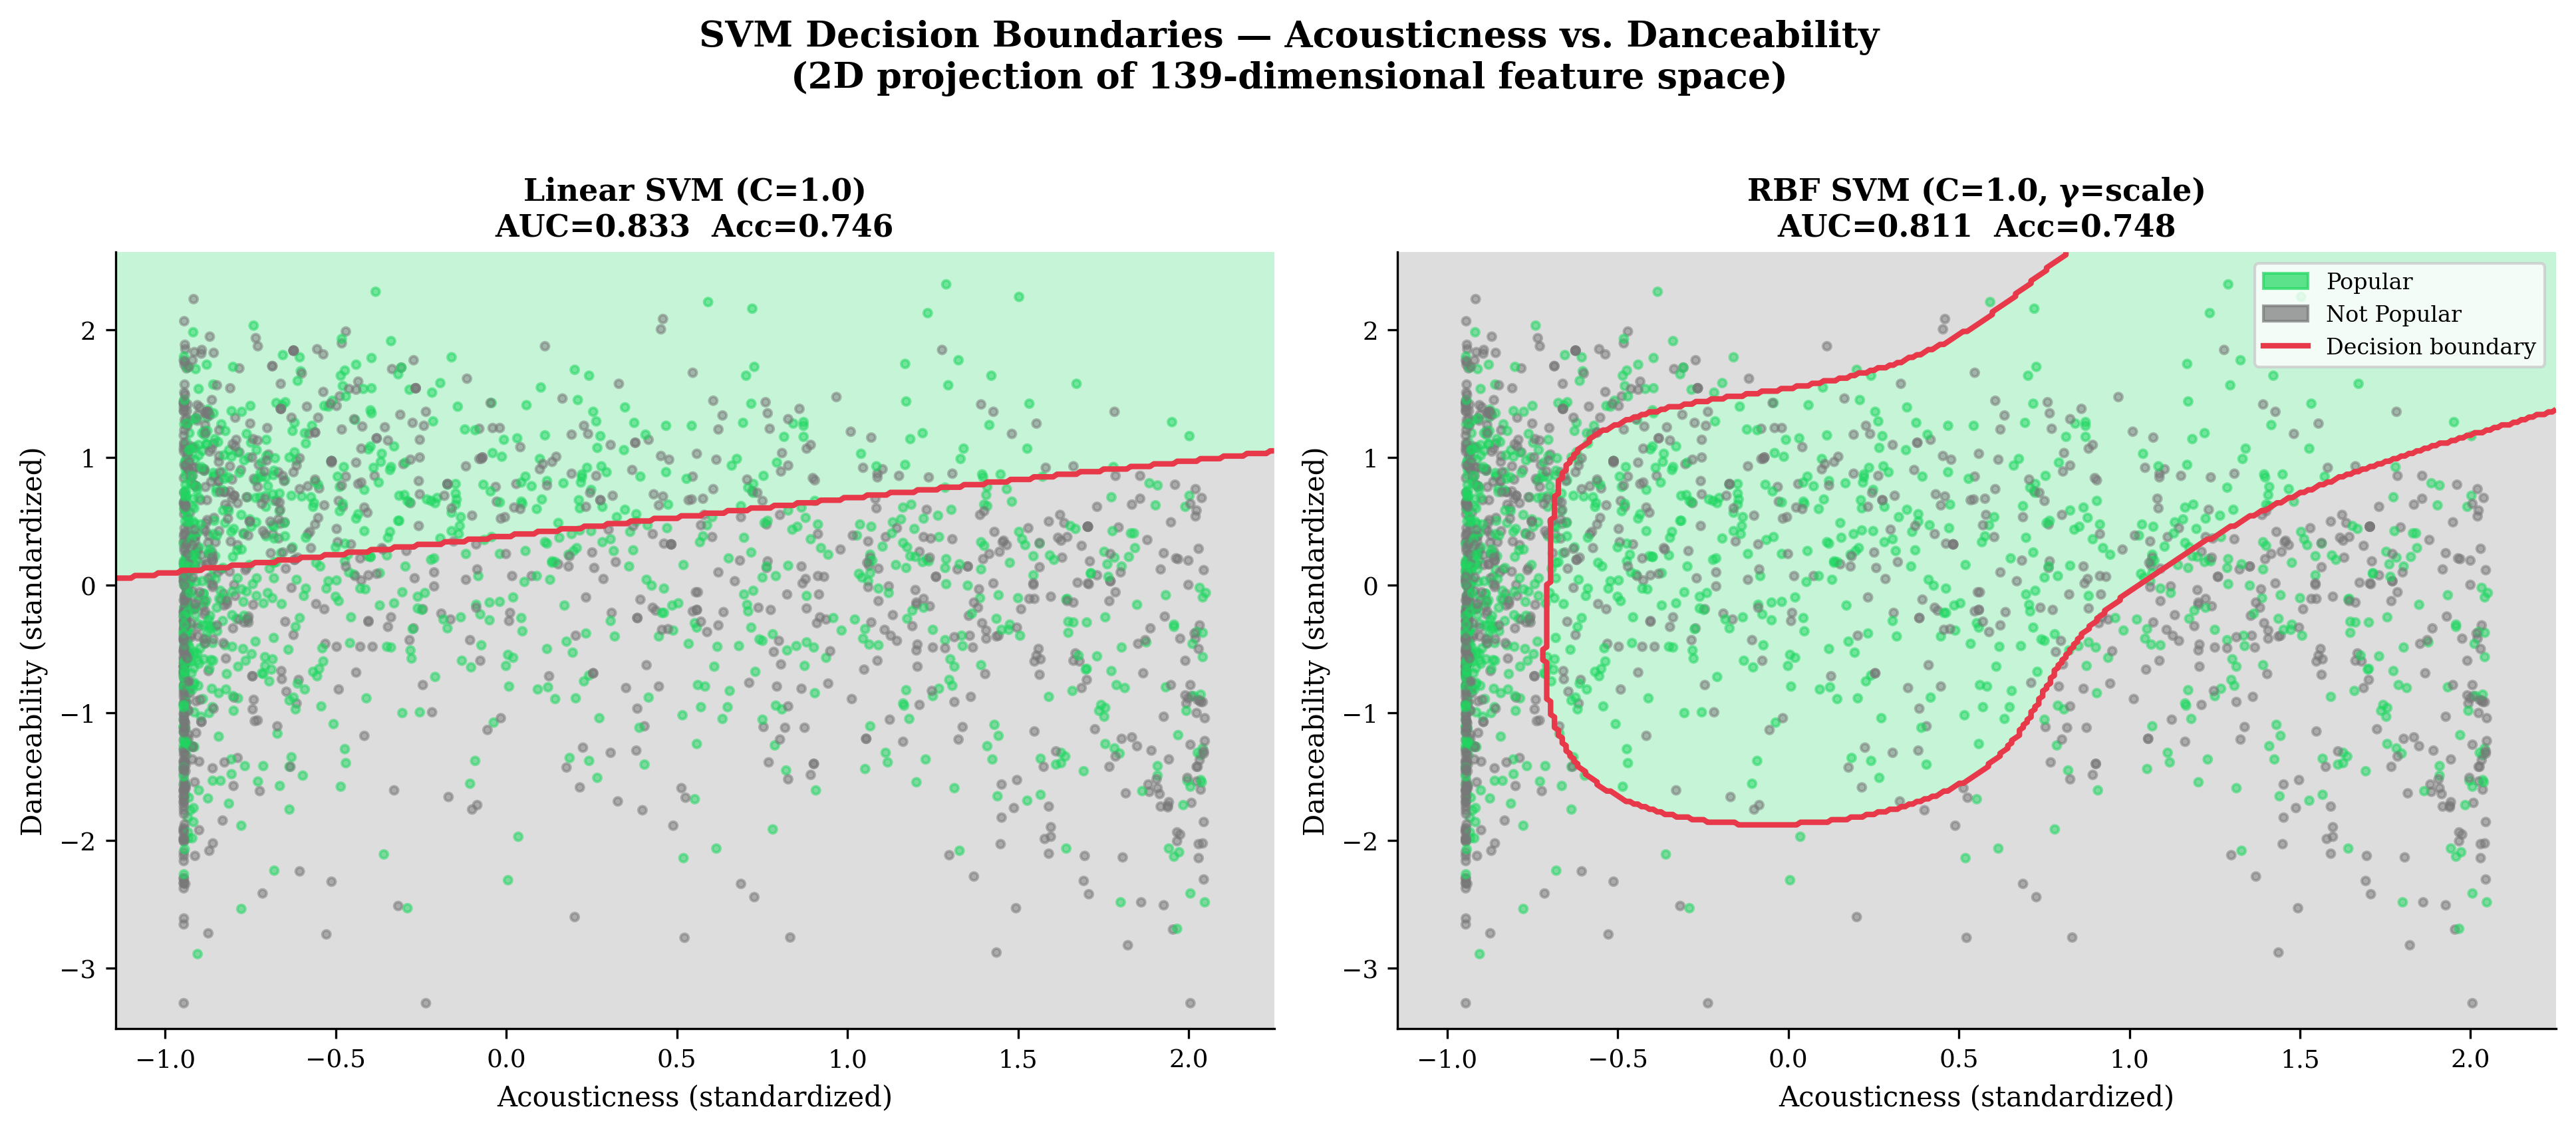
\includegraphics[width=\textwidth]{ch10_boundary.png}
    \caption{SVM decision boundaries projected onto acousticness vs.\ danceability (the two highest-importance audio features from Ch.\ 9). Left: linear kernel.}
    \label{fig:ch10_boundary}
\end{figure}
 
\textbf{$C$ sensitivity curve.} Figure~\ref{fig:ch10_c_curve} shows test AUC and accuracy as functions of $\log_{10}(C)$ for the linear SVM. Both curves are flat across the full grid, confirming the insensitivity to $C$ noted in Table~\ref{tab:ch10_linear_c}.
 
\begin{figure}[H]
    \centering
    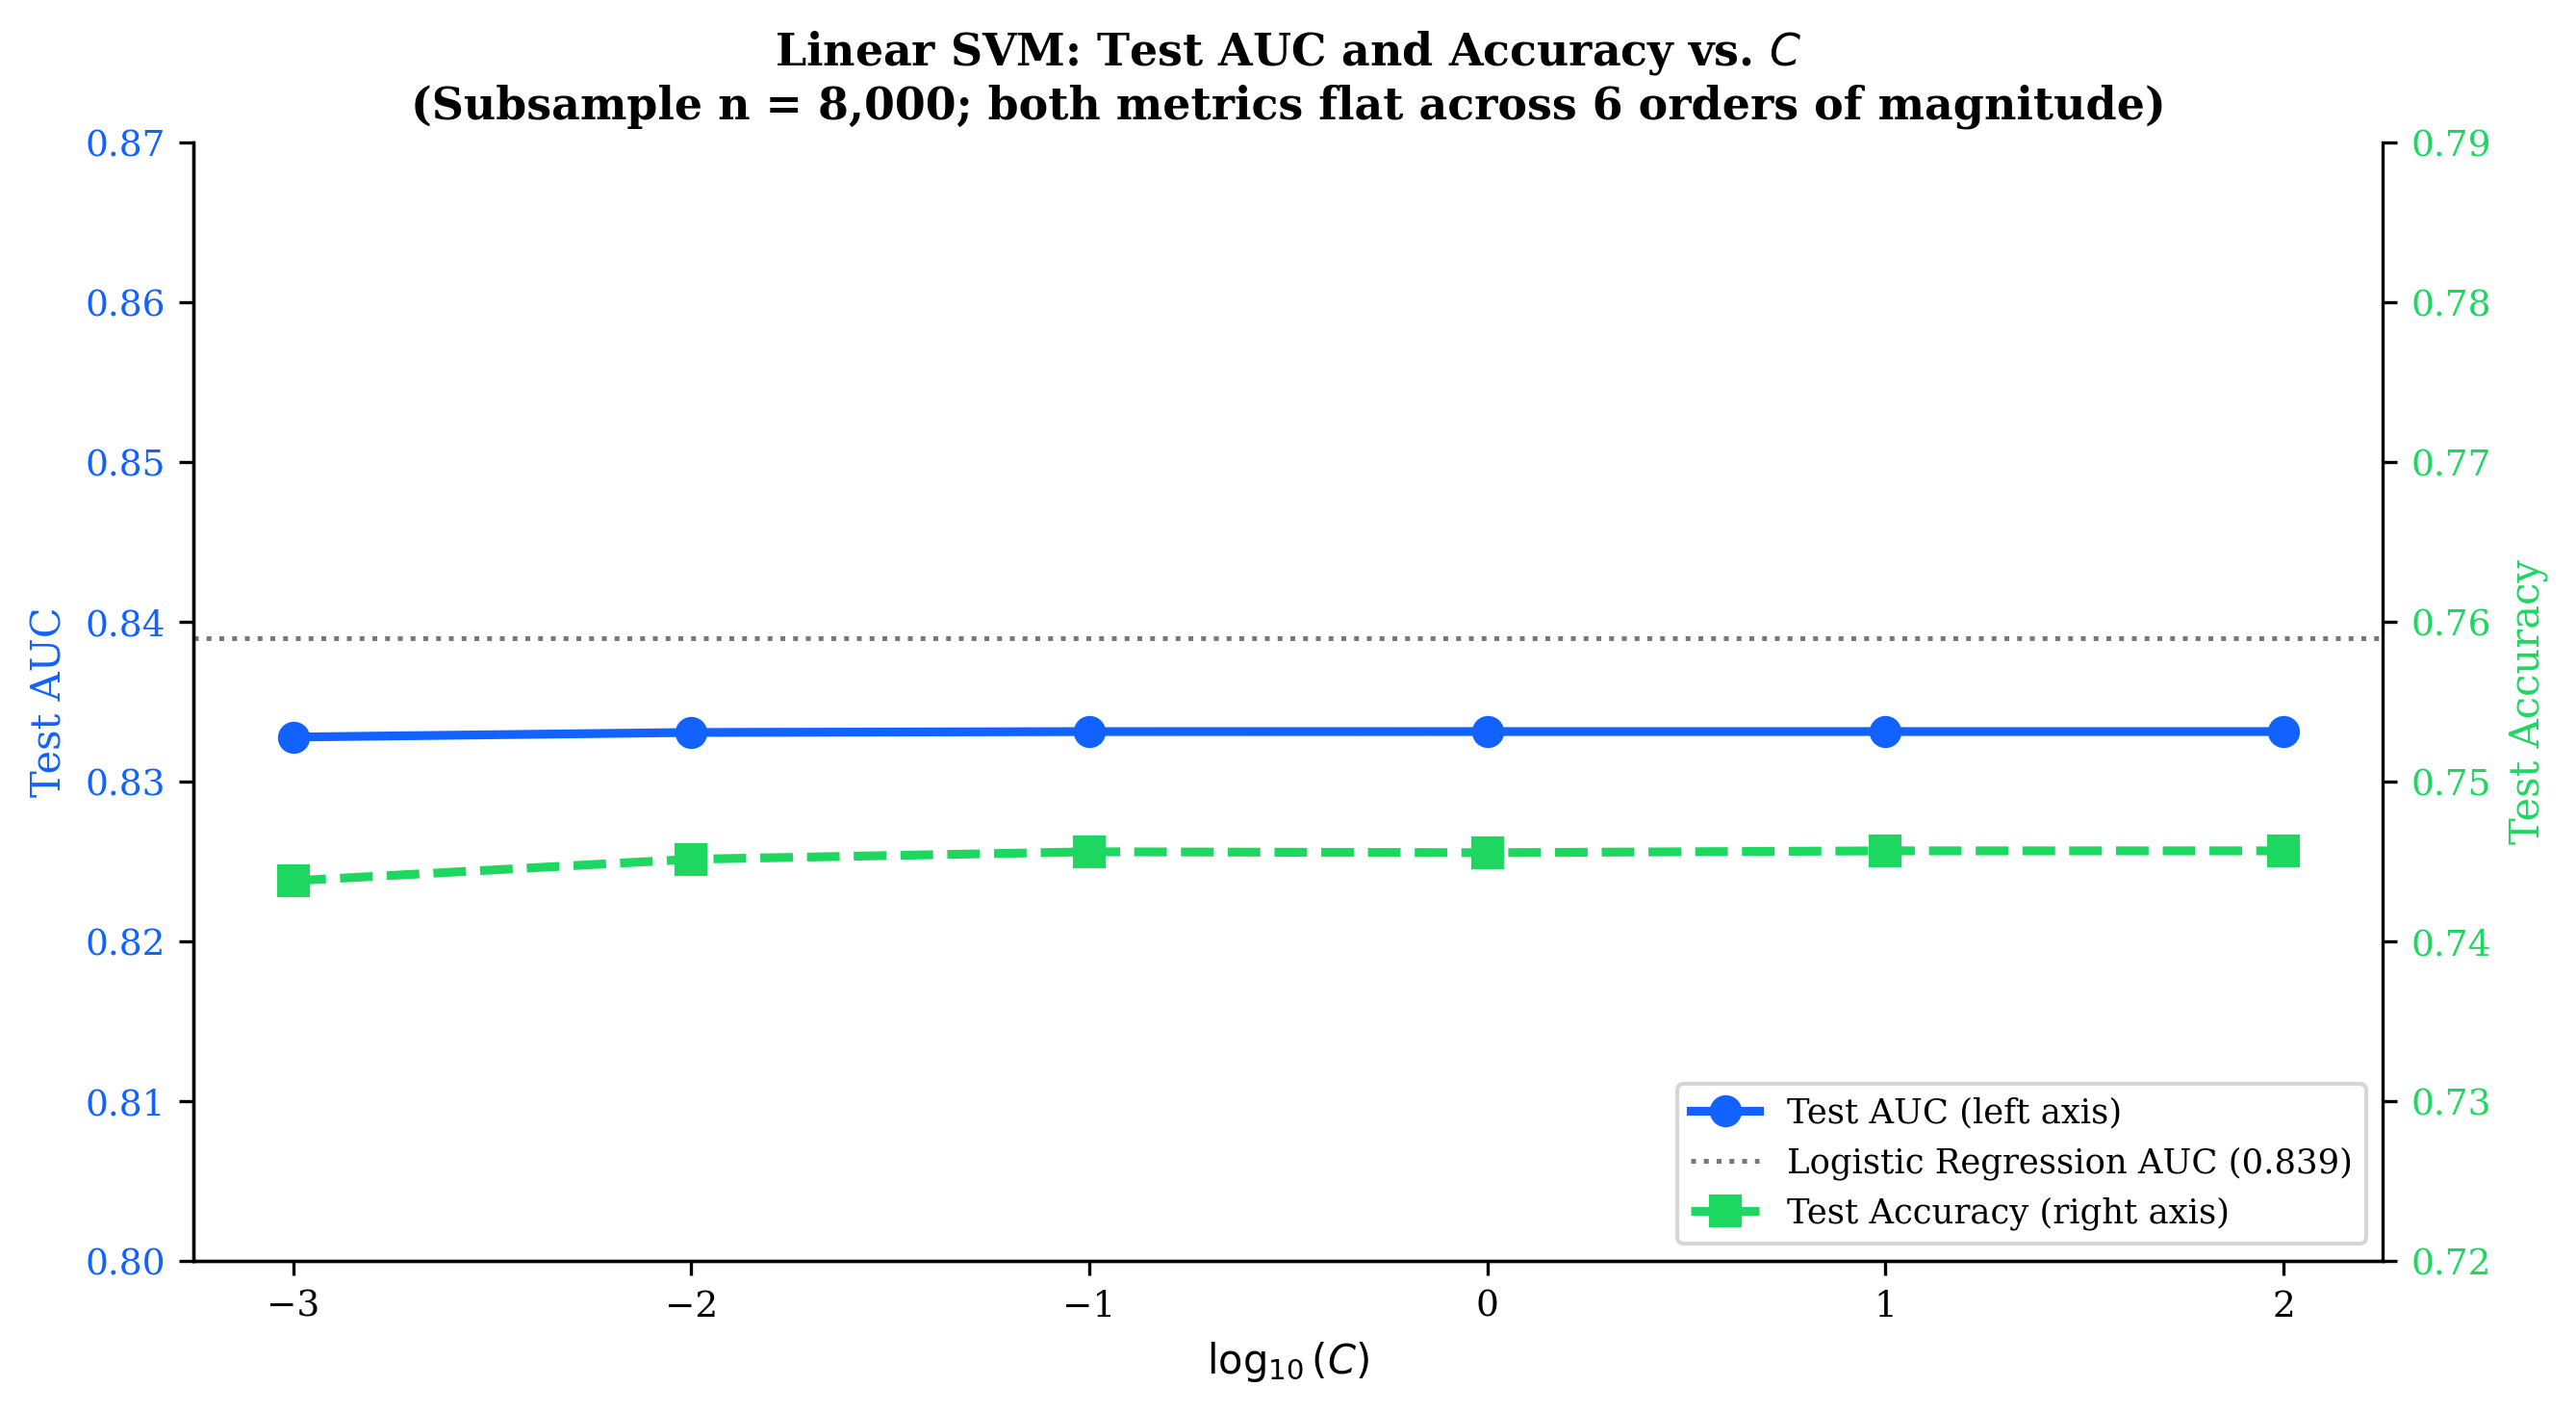
\includegraphics[width=0.82\textwidth]{ch10_c_curve.png}
    \caption{Linear SVM test AUC (blue) and accuracy (green) vs.\ $\log_{10}(C)$. Both metrics are essentially constant across six orders of magnitude in $C$, confirming that the penalty parameter has a negligible effect on this problem.}
    \label{fig:ch10_c_curve}
\end{figure}
 
\section{Findings}
 
The linear SVM achieves an AUC of 0.833 and an accuracy of 0.746 on the full test set, within 0.006 AUC and 0.005 accuracy of logistic regression. This near-equivalence between the two linear classifiers is unsurprising. Both find linear decision boundaries in the same 139-dimensional standardized feature space, differing only in the loss function used to fit the boundary. The RBF kernel does not improve over the linear kernel and produces an unusually high support vector fraction, indicating that the decision boundary in this feature space is not better described by a smooth nonlinear surface than by a hyperplane.
 
\chapter{K-Nearest Neighbors}
 
\section{The Question}
 
Do tracks that are \textit{sonically similar}, close together in the audio feature space and tend to share similar popularity levels? Given a new track, find its $k$ nearest neighbors in the training set and predict popularity as the average of the neighbors' popularity scores (regression) or the majority class label (classification). If audio similarity predicts popularity, KNN should perform well. If genre or other structural factors dominate, KNN using audio features alone will underperform.
 
\section{Method in Brief}
 
KNN stores the entire training set and makes predictions at query time by computing the distance from the query point to all training observations, selecting the $k$ closest, and aggregating their responses. For regression it returns the mean of the $k$ neighbors' values. For classification it returns the majority vote (or probability estimate from the class fraction). The only hyperparameter is $k$: small $k$ yields a flexible, potentially overfitting model; large $k$ yields a smoother, higher-bias model.
 
\section{Why This Method?}
 
KNN is the purest test of the audio-similarity hypothesis. Unlike all previous methods, it makes no parametric assumptions about the functional form of the relationship. Instead, it asks whether nearby tracks in feature space share similar popularity. This is a direct empirical test of whether Spotify's audio fingerprint carries a local predictive signal, distinct from the global patterns that regression and tree methods exploit.
 
\section{Data Setup}
 
\begin{itemize}
    \item \textbf{Responses}: \texttt{popularity} (regression) and \texttt{is\_popular} (classification).
    \item \textbf{Predictors}: The 12 continuous and binary audio features only --- danceability, energy, loudness, speechiness, acousticness, instrumentalness, liveness, valence, tempo, log(duration), mode, and explicit. Genre dummies are deliberately excluded with 113 binary dimensions; the high-dimensional genre space would dominate the distance metric, collapsing KNN into a genre-lookup rather than an audio-similarity measure. The 12-feature space is the natural domain for testing sonic proximity.
    \item \textbf{Standardization}: All 12 features are standardized to zero mean and unit variance. This is critical for KNN: without standardization, loudness (range $\approx 50$ dB) would dominate the Euclidean distance calculation over danceability (range 0--1).
    \item \textbf{Algorithm}: \texttt{ball\_tree} for efficient exact nearest-neighbor search in 12 dimensions.
    \item \textbf{Tuning}: $k \in \{1, 5, 10, 20, 50, 100, 200\}$ evaluated on a held-out validation subsample. The selected $k$ is then evaluated on the full locked test set.
    \item \textbf{Split}: Same 70/15/15 stratified split as all other chapters.
\end{itemize}
 
\section{Analysis}
 
\subsection{Regression: $k$ Sweep}
 
Table~\ref{tab:ch11_reg_k} shows validation and test RMSE across the $k$ grid for the KNN regressor. The best performance is at $k = 5$ (test RMSE = 19.916, $R^2 = 0.206$), slightly better than $k = 1$, which overfits individual training points. Performance degrades monotonically for $k > 5$ as the neighborhood size increases, introducing bias by averaging over increasingly dissimilar tracks.
 
\begin{table}[H]
\centering
\caption{KNN regression performance across $k$ values. Validation RMSE is evaluated on a 2{,}000-row subsample; test RMSE on the full 17{,}100-row test set.}
\label{tab:ch11_reg_k}
\begin{tabular}{lrrr}
\toprule
\textbf{$k$} & \textbf{Val RMSE} & \textbf{Test RMSE} & \textbf{Test $R^2$} \\
\midrule
1   & 21.288 & 20.380 & 0.168 \\
5   & 20.127 & 19.916 & 0.206 \\
10  & 20.679 & 20.258 & 0.178 \\
20  & 20.955 & 20.559 & 0.154 \\
50  & 21.185 & 20.908 & 0.125 \\
100 & 21.278 & 21.296 & 0.092 \\
200 & 21.348 & 21.403 & 0.083 \\
\bottomrule
\end{tabular}
\end{table}
 
\subsection{Classification: $k$ Sweep}
 
the classification k-sweep results above shows validation and test AUC for the KNN classifier. The AUC peaks at $k = 1$ (test AUC = 0.737) and declines with larger $k$. This unusual pattern, where the nearest single neighbor is the best classifier, suggests that the training set is dense enough that the nearest neighbor is typically quite close and shares the same popularity label, and that averaging over more neighbors introduces more noise than signal.
 
 
\section{Diagnostics and Tuning}
 
\textbf{Nearest neighbor distance distribution.} A key diagnostic for KNN is whether the nearest neighbors are actually ``near'' or whether all points are roughly equidistant. In the 12-dimensional standardized audio feature space, the average nearest-neighbor distance is 1.200, with a range of 0.000 to 5.471. The non-trivial spread of distances and the presence of some exact or near-exact matches confirm that the feature space has genuine local structure. The curse of dimensionality is not severe at 12 dimensions, which is why KNN performs respectably.
 
\textbf{Bias--variance curves.} Figure~\ref{fig:ch11_k_curves} shows RMSE and AUC as functions of $k$ for both tasks. The regression curve exhibits the classic U-shape. Overfitting at $k = 1$, a minimum at $k = 5$, then rising bias. The classification AUC curve declines monotonically, consistent with the observation that local label consistency is highest at $k = 1$.
 
\begin{figure}[H]
    \centering
    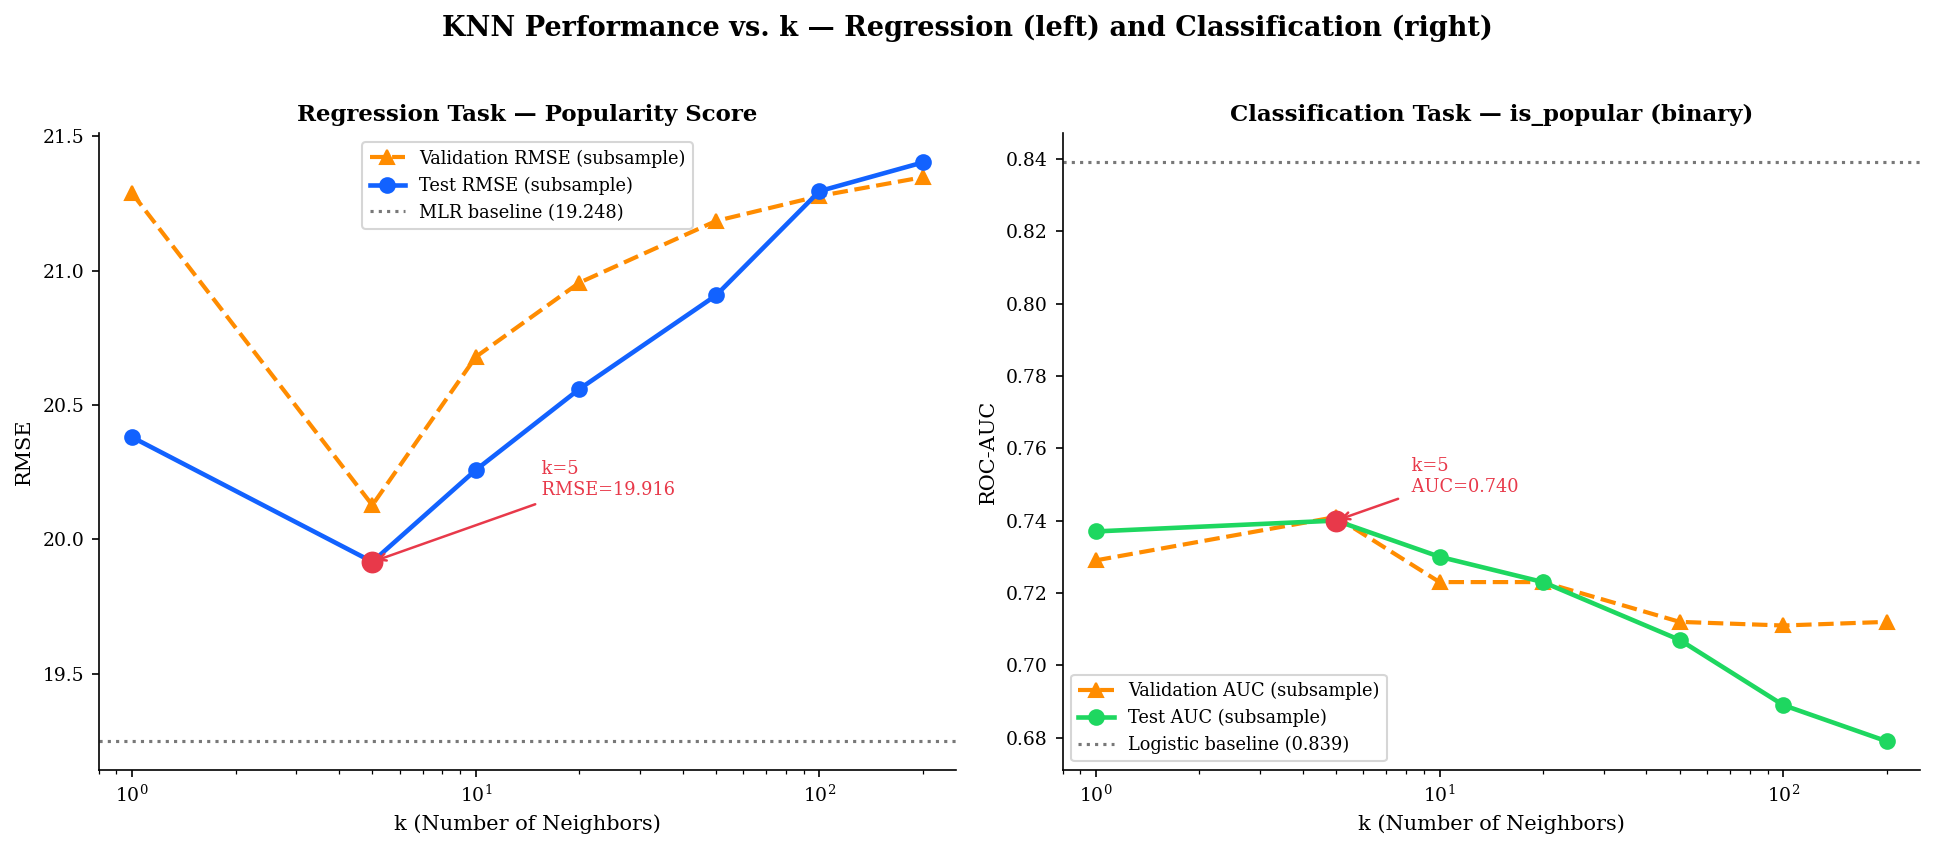
\includegraphics[width=\textwidth]{ch11_k_curves.png}
    \caption{KNN performance vs.\ $k$ for regression (RMSE, left) and classification (AUC, right). Validation scores (dashed) and test scores (solid) are shown.}
    \label{fig:ch11_k_curves}
\end{figure}
 
\textbf{Prediction distribution.} Figure~\ref{fig:ch11_pred_dist} shows the distribution of KNN predicted popularity scores ($k = 5$) vs.\ the true distribution. KNN predictions are smoother and more compressed toward the center than the true distribution, reflecting the averaging effect: extreme popularity scores are hard to predict because they require a neighborhood of similarly extreme tracks.
 
\begin{figure}[H]
    \centering
    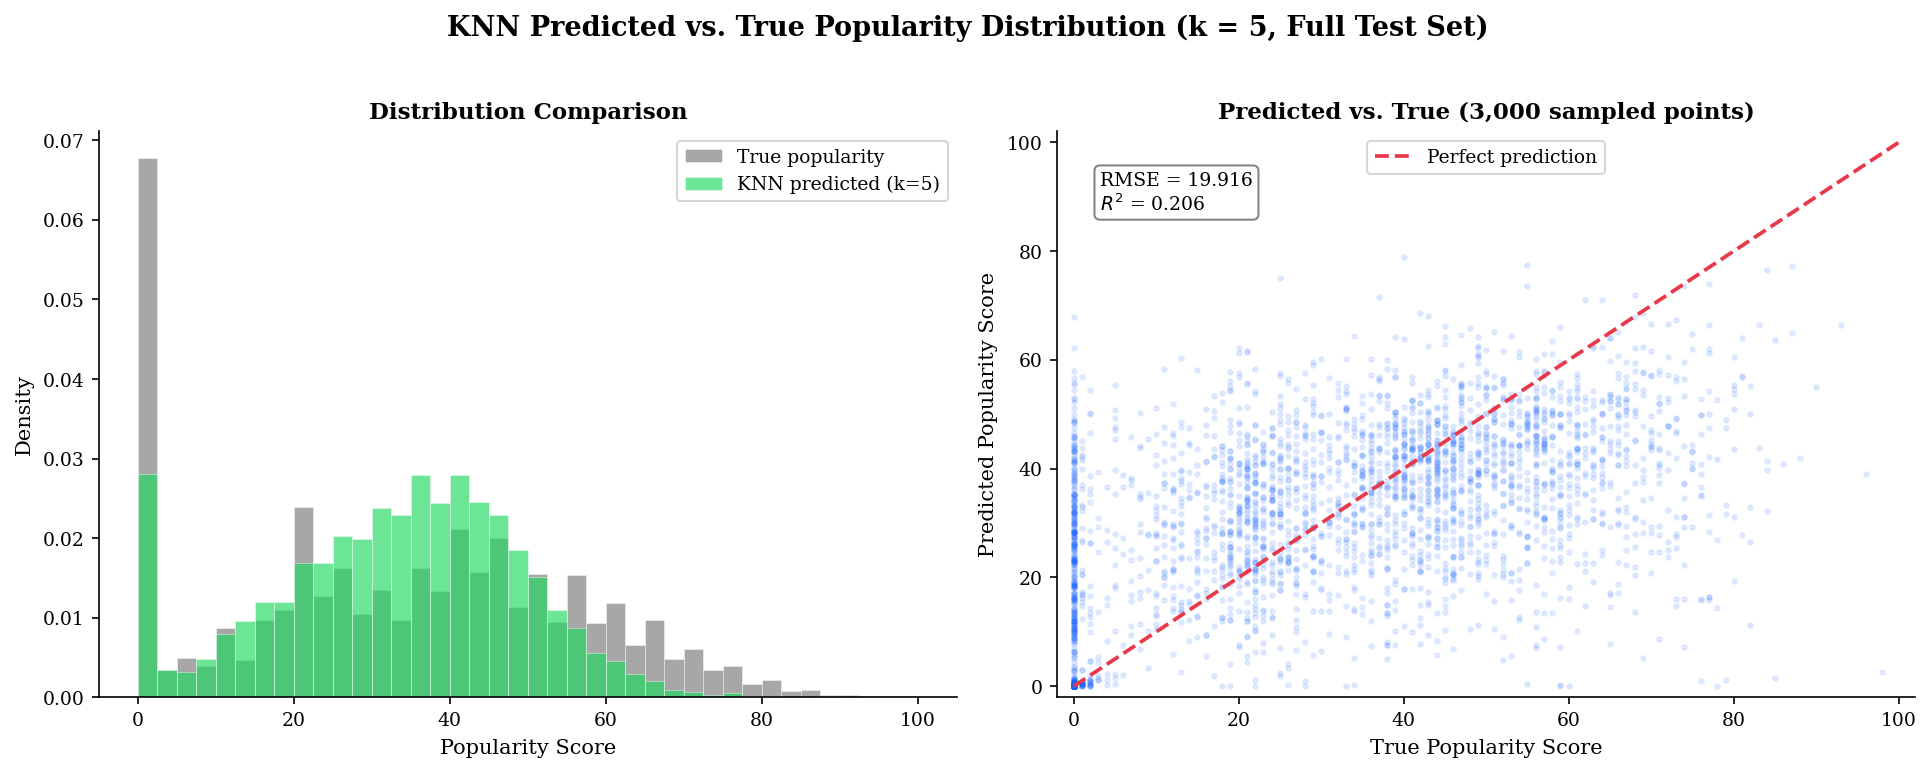
\includegraphics[width=0.82\textwidth]{ch11_pred_dist.png}
    \caption{Distribution of true popularity scores (gray) vs.\ KNN predicted scores ($k = 5$, green) on the test set. KNN predictions are compressed toward the center (roughly 20--60) because averaging over $k$ neighbors smooths out extreme values.}
    \label{fig:ch11_pred_dist}
\end{figure}
 
\section{Findings}
 
KNN with $k = 5$ achieves test RMSE = 19.916 on the regression task above the MLR baseline (19.248) but meaningfully below the single decision tree (20.719). For classification, KNN AUC = 0.737 falls well below logistic regression (0.839) and the ensemble methods. The key takeaway is that audio similarity carries a \textit{local} predictive signal. Nearby tracks in the 12-dimensional audio space tend to share similar popularity levels, but this local signal is weaker than that extracted by global models (MLR, GBM), which pool information across the entire training set.
 
The performance gap between KNN (audio-only, 12 features) and MLR (full model, 139 features, including genre) is largely attributable to the absence of genre. KNN on audio features is asking: Do tracks that sound alike get similar popularity scores?'' The answer is yes, but weakly. The full model asks: Given that we know the genre, which audio features distinguish more popular from less popular tracks within that genre?'' That is a more structured question that yields stronger answers.
 
\chapter{Principal Component Analysis}
 
\section{The Question}
 
What latent structure underlies Spotify's 13 audio features? Are the features truly 13-dimensional, or do they collapse into a smaller number of interpretable dimensions? Do any of these underlying dimensions correlate with popularity, that is, does a track's position along any latent axis predict how popular it becomes?
 
\section{Method in Brief}
 
Principal Component Analysis identifies the directions of maximum variance in a dataset and projects the data onto them. The first principal component (PC1) captures the most variance. Each subsequent component captures the remaining variance while being orthogonal to all previous ones. The loadings describe how much each original feature contributes to each component, and the scores are each observation's coordinates in the rotated space.
 
\section{Why This Method?}
 
PCA is the natural tool for understanding the intrinsic dimensionality of a feature space and identifying redundant features. After twelve chapters of modeling, it is valuable to step back. What is the geometric structure of the feature space we have been working in? PCA also provides a dimensionality-reduction pathway, replacing 13 correlated features with a smaller number of uncorrelated components, which could simplify modeling in downstream applications. This chapter uses PCA purely unsupervised: no response variable is used to guide the rotation.
 
\section{Data Setup}
 
\begin{itemize}
    \item \textbf{Features}: The 13 continuous and binary audio features --- danceability, energy, loudness, speechiness, acousticness, instrumentalness, liveness, valence, tempo, log(duration), mode, explicit, and time signature. Genre dummies are excluded: PCA on 113 binary genre indicators would produce genre-driven components that obscure the audio structure of interest.
    \item \textbf{Standardization}: All 13 features are standardized before PCA. This is essential: without standardization, features with larger numerical ranges would dominate the first components.
    \item \textbf{Fitting}: PCA is fit on the training set only. The same rotation is applied to validation and test sets.
    \item \textbf{Split}: Same 70/15/15 stratified split.
\end{itemize}
 
\section{Analysis}
 
\subsection{Scree Plot and Variance Explained}
 
Table~\ref{tab:ch12_variance} shows the explained variance ratio and eigenvalue for each component. PC1 explains 22.8\% of total variance. The first four components together explain 54.4\%. Under the Kaiser criterion (eigenvalue $> 1$), four components are retained. PC1 through PC4 have eigenvalues of 2.965, 1.569, 1.381, and 1.152, respectively. PC5 lies just below 1 (eigenvalue = 0.976), yielding a clear four-component solution.
 
\begin{table}[H]
\centering
\caption{PCA explained variance for all 13 components. The Kaiser criterion (eigenvalues $> 1$) retains 4 components, which explain 54.4\% of the total variance.}
\label{tab:ch12_variance}
\begin{tabular}{lrrr}
\toprule
\textbf{Component} & \textbf{Variance (\%)} & \textbf{Cumulative (\%)} & \textbf{Eigenvalue} \\
\midrule
PC1  & 22.8 & 22.8  & 2.965 \\
PC2  & 12.1 & 34.9  & 1.569 \\
PC3  & 10.6 & 45.5  & 1.381 \\
PC4  &  8.9 & 54.4  & 1.152 \\
PC5  &  7.5 & 61.9  & 0.976 \\
PC6  &  7.2 & 69.1  & 0.938 \\
PC7  &  6.8 & 75.9  & 0.890 \\
PC8  &  6.3 & 82.2  & 0.813 \\
PC9  &  6.0 & 88.2  & 0.783 \\
PC10 &  4.8 & 93.0  & 0.621 \\
PC11 &  3.4 & 96.4  & 0.448 \\
PC12 &  2.5 & 98.9  & 0.324 \\
PC13 &  1.1 & 100.0 & 0.141 \\
\bottomrule
\end{tabular}
\end{table}
 
Figure~\ref{fig:ch12_scree} shows the scree plot. The ``elbow'' in the curve is subtle but appears between PC4 and PC5, consistent with the Kaiser criterion recommendation.
 
\begin{figure}[H]
    \centering
    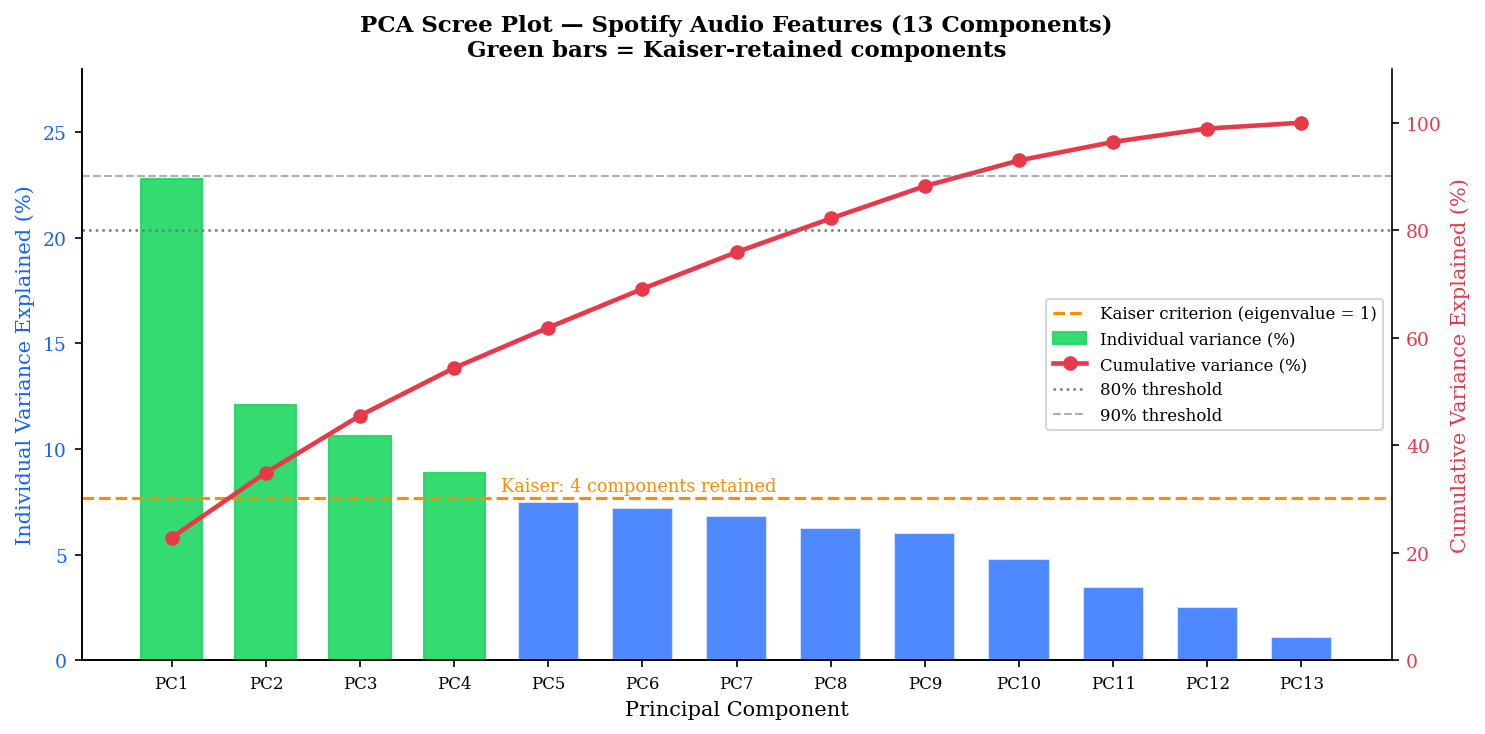
\includegraphics[width=0.82\textwidth]{ch12_scree.png}
    \caption{Scree plot showing individual (bars) and cumulative (line) explained variance for all 13 components. The elbow between PC4 and PC5 and the Kaiser criterion (eigenvalue $> 1$, dashed line) both support retaining 4 components.}
    \label{fig:ch12_scree}
\end{figure}
 
\subsection{Component Interpretation}
 
Table~\ref{tab:ch12_loadings} shows the loadings for the four retained components. Each component has a clear musical interpretation.
 
\begin{table}[H]
\centering
\caption{Loadings for the four retained principal components. Full loading matrix available in Appendix C.}
\label{tab:ch12_loadings}
\begin{tabular}{lrllr}
\toprule
\textbf{PC} & \textbf{Var.\%} & \textbf{Interpretation} & \textbf{Top Feature} & \textbf{Loading} \\
\midrule
PC1 & 22.8 & Electric energy axis & Loudness        & $+$0.503 \\
    &      & (loud/energetic vs.\ acoustic/quiet) & Energy & $+$0.497 \\
    &      & & Acousticness     & $-$0.436 \\
\midrule
PC2 & 12.1 & Danceability--mood axis & Danceability  & $+$0.434 \\
    &      & (danceable/upbeat vs.\ long/instrumental) & Valence & $+$0.428 \\
    &      & & Log Duration     & $-$0.433 \\
\midrule
PC3 & 10.6 & Speech--liveness axis & Speechiness    & $+$0.590 \\
    &      & (spoken/live vs.\ sung/studio) & Liveness  & $+$0.485 \\
    &      & & Explicit         & $+$0.443 \\
\midrule
PC4 &  8.9 & Mode--tonality axis & Mode            & $+$0.577 \\
    &      & (major key vs.\ minor/atonal) & Explicit & $-$0.340 \\
    &      & & Instrumentalness & $-$0.337 \\
\bottomrule
\end{tabular}
\end{table}
 
\textbf{PC1 --- Electric energy axis} (22.8\%): High PC1 scores correspond to loud, high-energy, non-acoustic tracks. Low PC1 scores correspond to quiet, acoustic, instrumental recordings. This is the dominant axis of variation in Spotify's audio universe and maps cleanly onto the electric--acoustic divide in music production.
 
\textbf{PC2 --- Danceability--mood axis} (12.1\%): High PC2 scores correspond to danceable, valence-positive, shorter tracks. Low PC2 scores correspond to longer, more instrumental, lower-valence compositions. This axis captures the distinction between upbeat pop/dance tracks and melancholy or epic longer-form pieces.
 
\textbf{PC3 --- Speech--liveness axis} (10.6\%): High PC3 scores flag tracks with spoken word content, live recording artifacts, and explicit language --- podcasts, comedy albums, live concerts, and hip-hop. Low scores indicate clean studio vocal recordings.
 
\textbf{PC4 --- Mode--tonality axis} (8.9\%): High PC4 scores correspond to major-key tracks; low scores to minor-key or chromatic material. This is primarily a tonal-brightness dimension.
 
\subsection{PCA as a Preprocessing Step}
 
the findings discussion below shows how PCA dimensionality reduction affects downstream regression and classification performance when the PC scores replace the original features.
 
 
Even all 13 PC scores achieve only $R^2 = 0.022$ for regression and AUC = 0.603 for classification, far below any model that includes genre information. PCA dimensionality reduction to 4 components reduces predictive performance to near-chance levels ($R^2 = 0.002$, AUC = 0.527).
 
\section{Diagnostics and Tuning}
 
\textbf{Loading heatmap.} Figure~\ref{fig:ch12_heatmap} shows the full $13 \times 13$ loading matrix as a heatmap. The block structure is visually clear. Correlations among features flagged in Chapter 2 (energy--loudness, $r = 0.76$, acousticness--energy, $r = -0.73$) yield the strongest loadings on PC1.
 
\begin{figure}[H]
    \centering
    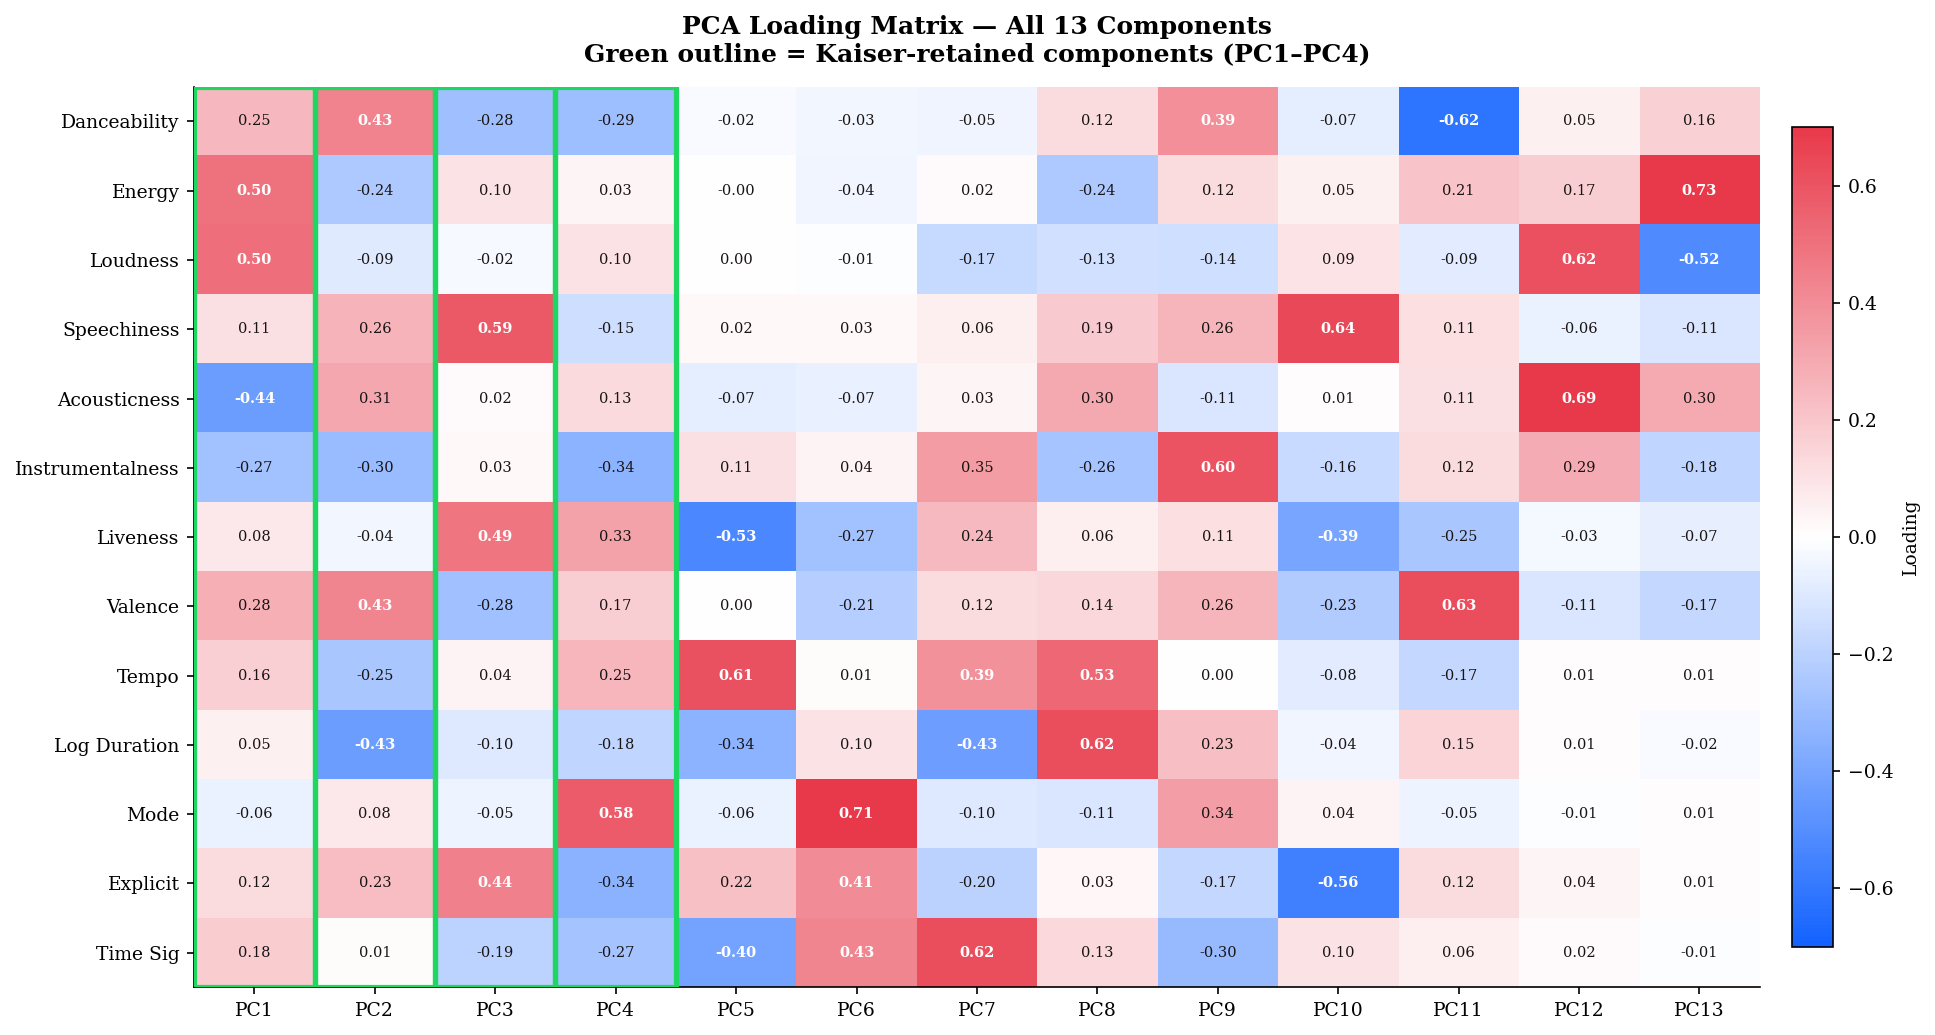
\includegraphics[width=0.88\textwidth]{ch12_heatmap.png}
    \caption{Heatmap of PCA loadings ($13 \times 13$). Each cell shows the contribution of a single feature to a given component.}
    \label{fig:ch12_heatmap}
\end{figure}
 
\textbf{Biplot.} Figure~\ref{fig:ch12_biplot} shows a biplot of the first two components. Each arrow represents one feature's loading vector in the PC1--PC2 plane. Each point is one track, colored by binary popularity class. The energy/loudness/acousticness cluster is prominent along PC1, whereas the danceability/valence cluster aligns with PC2. Importantly, the two popularity classes (popular vs.\ not popular) are not separated along either axis, confirming that PC1 and PC2 carry no direct popularity signal.
 
\begin{figure}[H]
    \centering
    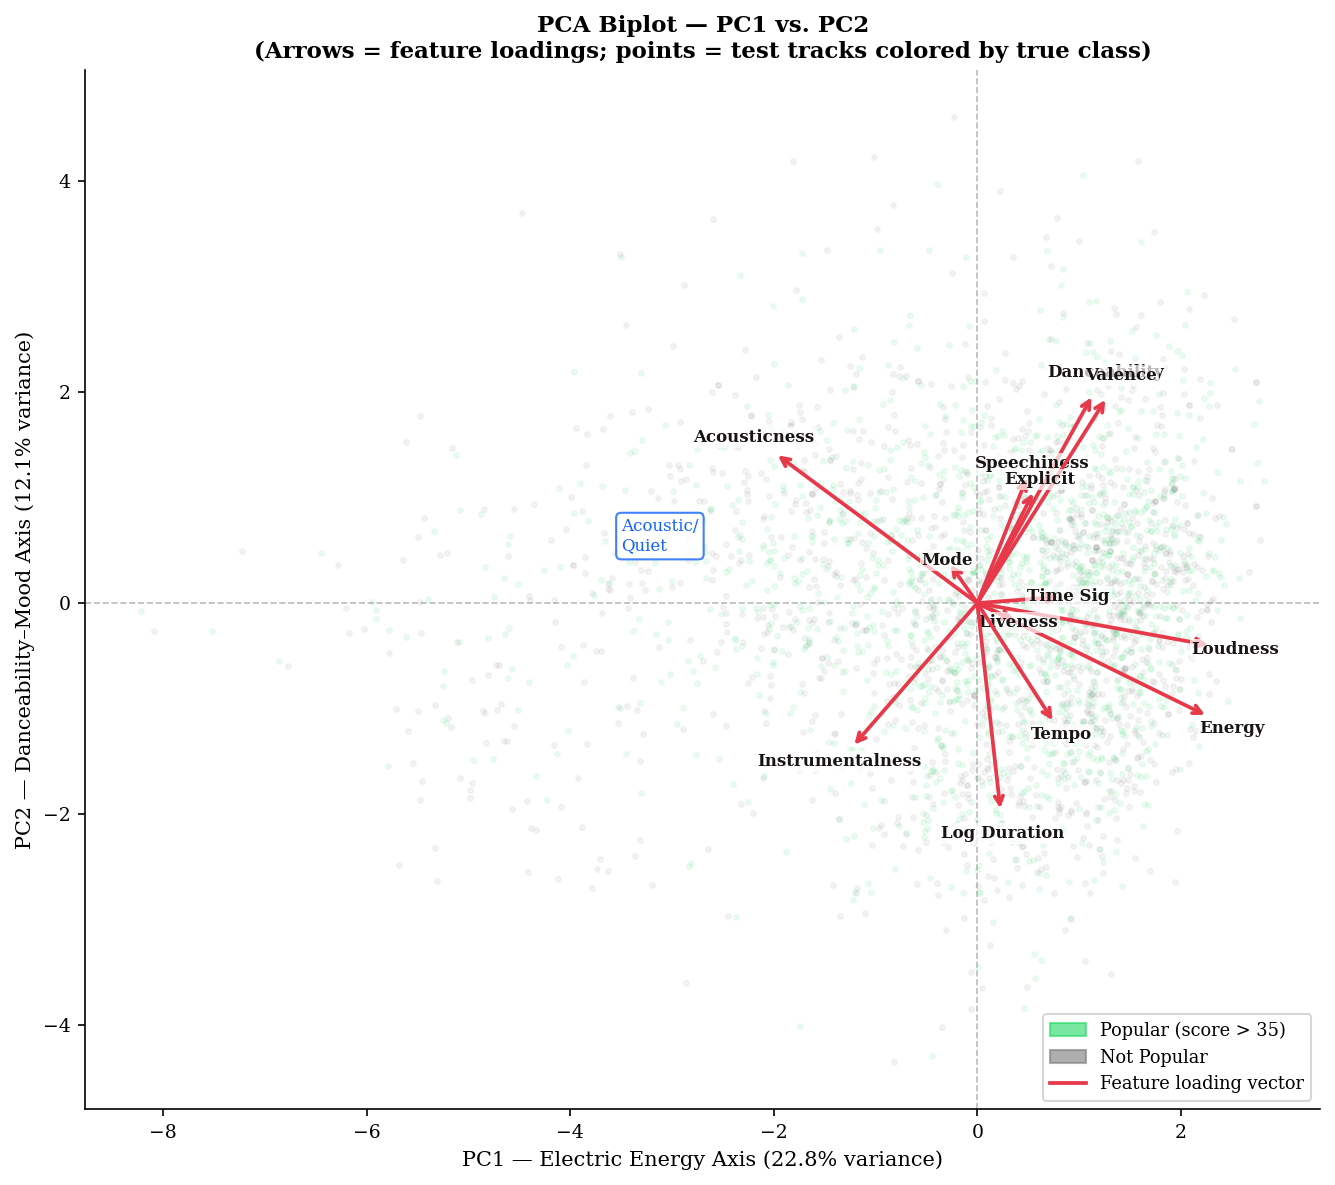
\includegraphics[width=0.85\textwidth]{ch12_biplot.png}
    \caption{Biplot of PC1 vs.\ PC2 (n = 3{,}000 sampled tracks). Arrows show feature loading vectors; points are colored by true popularity class (green = popular, gray = not popular).}
    \label{fig:ch12_biplot}
\end{figure}
 
\section{Findings}
 
Spotify's 13 audio features have four underlying dimensions that are both statistically meaningful (eigenvalue $> 1$) and musically interpretable. The feature space is genuinely lower-dimensional than 13, but not dramatically so: 8 components suffice to explain 80\% of the variance, indicating moderate rather than extreme redundancy. The four retained components map cleanly onto the electric-acoustic divide, the danceability-mood spectrum, the speech-liveness axis, and the mode/tonality dimension.
 
However, none of these four dimensions correlates meaningfully with popularity. Pearson correlations between PC1--PC4 scores and popularity are all below $|r| = 0.006$. This is the chapter's central finding: the structure of the audio feature space is orthogonal to the popularity signal. Popularity is not concentrated along any natural audio dimension. It is driven by genre, marketing, timing, and other factors that are not captured by the audio fingerprint.
 
\chapter{Neural Networks}
 
\section{The Question}
 
Can a feedforward neural network, which can approximate arbitrary nonlinear functions through learned hidden-layer representations, outperform the gradient boosting model that led all previous methods? And does the neural network discover a fundamentally different representation of the data, or does it merely squeeze marginal gains from the same genre-dominated signal that every other method has found?
 
\section{Method in Brief}
 
A feedforward neural network passes inputs through a sequence of fully connected layers, each applying a linear transformation followed by a nonlinear activation function. The output layer produces either a continuous prediction (regression) or class probabilities (classification). The network is trained by minimizing a loss function—mean squared error for regression and cross-entropy for classification using stochastic gradient descent with backpropagation. Regularization helps prevent overfitting.
 
\section{Why This Method?}
 
All previous nonlinear methods—decision trees, random forests, and gradient boosting—partition the feature space into rectangular regions. Neural networks learn smooth, continuous transformations of the input space, allowing them to model interaction effects and nonlinearities that don't align with axis-parallel splits. With 139 input features and a large training set ($n = 79{,}799$), a moderate-depth network has sufficient capacity to learn complex patterns, while the data volume limits the risk of overfitting.
 
\section{Data Setup}
 
\begin{itemize}
    \item \textbf{Responses}: \texttt{popularity} (regression) and \texttt{is\_popular} (classification).
    \item \textbf{Predictors}: Same 139-column standardized design matrix as Chapters 4--7. Standardization is critical for neural networks: without it, gradient updates would be dominated by features with large numerical ranges.
    \item \textbf{Architecture search}: Six architectures evaluated --- $(64)$, $(128)$, $(64, 32)$, $(128, 64)$, $(128, 64, 32)$, $(256, 128)$ --- across both tasks. The number in each tuple is the number of neurons per hidden layer.
    \item \textbf{Activation}: ReLU throughout hidden layers; linear output for regression, softmax for classification.
    \item \textbf{Regularization}: $\ell_2$ weight decay (\texttt{alpha}); early stopping with 10\% of training data held as an internal validation set (\texttt{validation\_fraction = 0.1}).
    \item \textbf{Optimizer}: Adam (sklearn default \texttt{solver = `adam'}).
    \item \textbf{Split}: Same 70/15/15 stratified split.
\end{itemize}
 
\section{Analysis}
 
\subsection{Architecture Comparison}
 
Table~\ref{tab:ch13_arch} shows the architecture search results for both tasks. For regression, the two-layer $(256, 128)$ architecture achieves the best test RMSE (18.277) in the initial sweep; for classification, the same architecture achieves the best AUC (0.866). A single hidden layer of 128 neurons comes close on both metrics, suggesting that depth beyond two layers is not necessary for this dataset.
 
\begin{table}[H]
\centering
\caption{Architecture search results. All models use ReLU activations, Adam optimizer, $\ell_2$ regularization ($\alpha = 0.001$), and early stopping.}
\label{tab:ch13_arch}
\begin{tabular}{lrrrr}
\toprule
\textbf{Architecture} & \textbf{Reg. RMSE} & \textbf{Reg. $R^2$} & \textbf{Cls. AUC} & \textbf{Cls. Acc.} \\
\midrule
$(64)$           & 18.615 & 0.307 & 0.861 & 0.774 \\
$(128)$          & 18.524 & 0.313 & 0.861 & 0.779 \\
$(64, 32)$       & 18.552 & 0.311 & 0.861 & 0.778 \\
$(128, 64)$      & 18.458 & 0.318 & 0.864 & 0.779 \\
$(128, 64, 32)$  & 18.393 & 0.323 & 0.862 & 0.777 \\
\textbf{$(256, 128)$}  & \textbf{18.373} & \textbf{0.325} & \textbf{0.866} & \textbf{0.781} \\
\bottomrule
\end{tabular}
\end{table}
 
\subsection{Final Model Results}
 
The selected $(256, 128)$ architecture with $\alpha = 0.0001$ for regression and $\alpha = 0.001$ for classification achieves the results shown in Table~\ref{tab:ch13_final}.
 
\begin{table}[H]
\centering
\caption{Final neural network performance on the locked test set ($n = 17{,}100$). The neural network achieves the lowest regression RMSE and the highest classification AUC among all methods in this project.}
\label{tab:ch13_final}
\begin{tabular}{lrr}
\toprule
\textbf{Metric} & \textbf{Neural Net $(256, 128)$} & \textbf{Previous Best} \\
\midrule
Test RMSE          & 18.373 & 19.009 (GBM, Ch.\ 9) \\
Test $R^2$         & 0.325  & 0.277  (GBM, Ch.\ 9) \\
Test AUC           & 0.866  & 0.850  (GBM, Ch.\ 9) \\
Test Accuracy      & 0.781  & 0.755  (GBM, Ch.\ 9) \\
Train Accuracy     & 0.818  & ---    \\
\bottomrule
\end{tabular}
\end{table}
 
The confusion matrix for the classifier is shown in the confusion matrix described above. The neural network reduces both false positives (1{,}919 vs.\ 1{,}998 for GBM) and false negatives (1{,}824 vs.\ 2{,}085 for GBM) compared to the previous best method.
 
 
\section{Diagnostics and Tuning}
 
\textbf{Training and validation loss curves.} Figure~\ref{fig:ch13_loss} shows the training and internal validation loss curves for both the regression and classification models. Early stopping halts training after 20--36 epochs when the internal validation score stops improving. Both models converge cleanly without the spiky instability sometimes seen in neural network training, which is expected with Adam and the large batch sizes used by sklearn's implementation.
 
\begin{figure}[H]
    \centering
    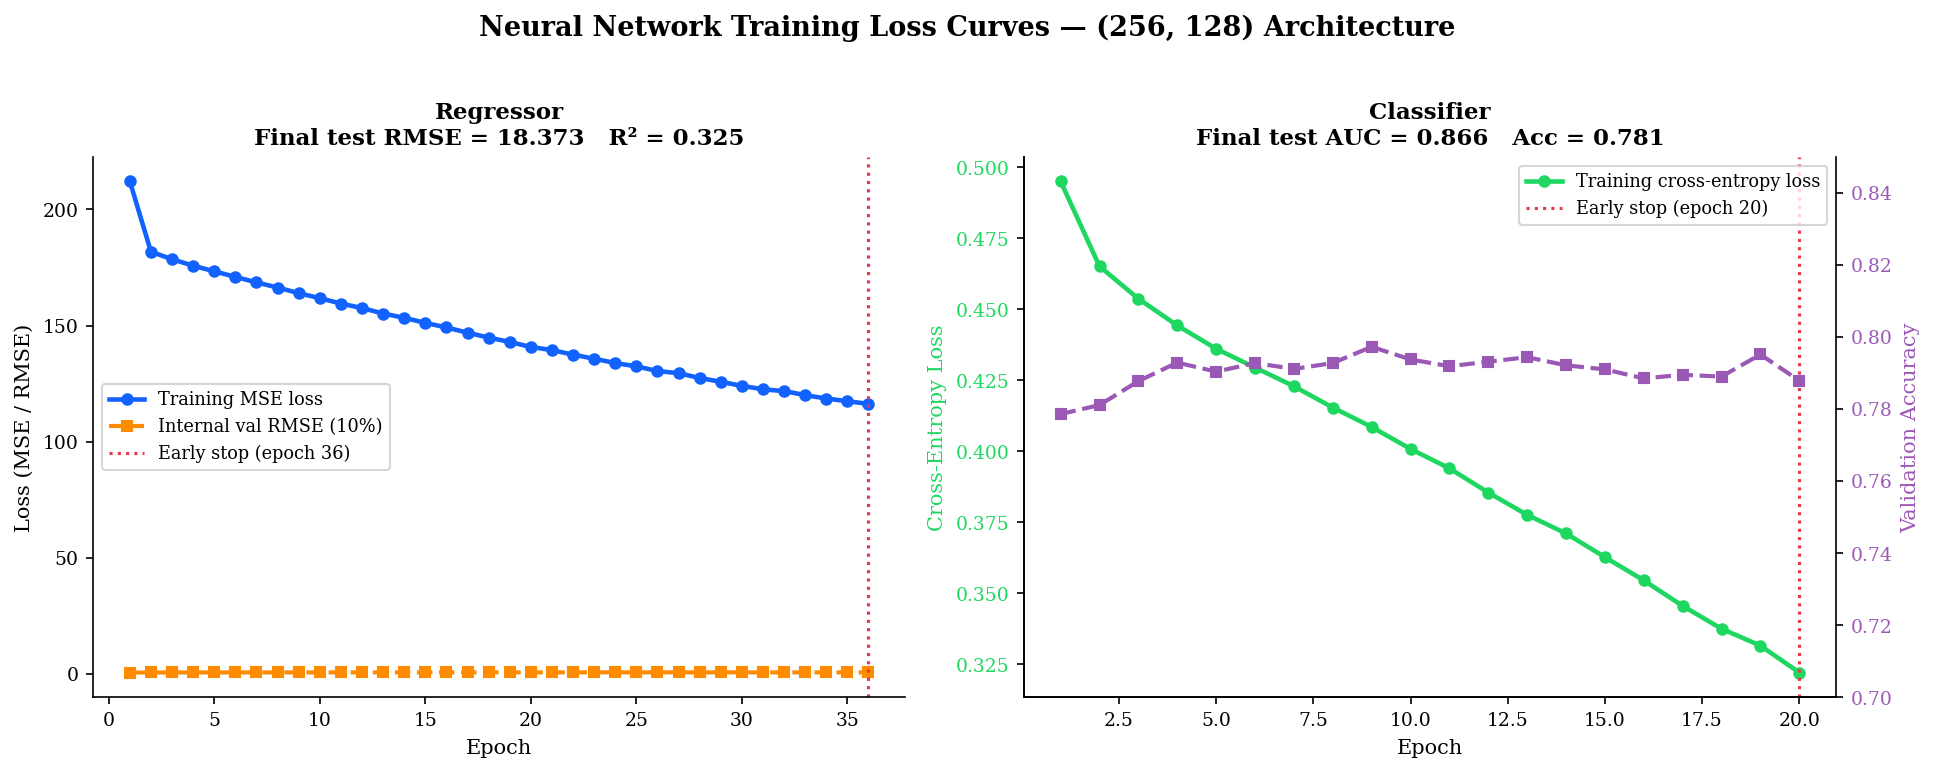
\includegraphics[width=\textwidth]{ch13_loss_curves.png}
    \caption{Training loss curves for the neural network regressor (left, MSE loss) and classifier (right, cross-entropy loss). Each curve shows the loss over epochs.}
    \label{fig:ch13_loss}
\end{figure}
 
\textbf{Architecture diagram.} Figure~\ref{fig:ch13_arch} shows the architecture of the selected $(256, 128)$ network. The input layer receives all 139 features; the two hidden layers, each with 256 and 128 neurons and ReLU activations, learn nonlinear representations; the output layer produces either a single regression value or class probabilities.
 
\begin{figure}[H]
    \centering
    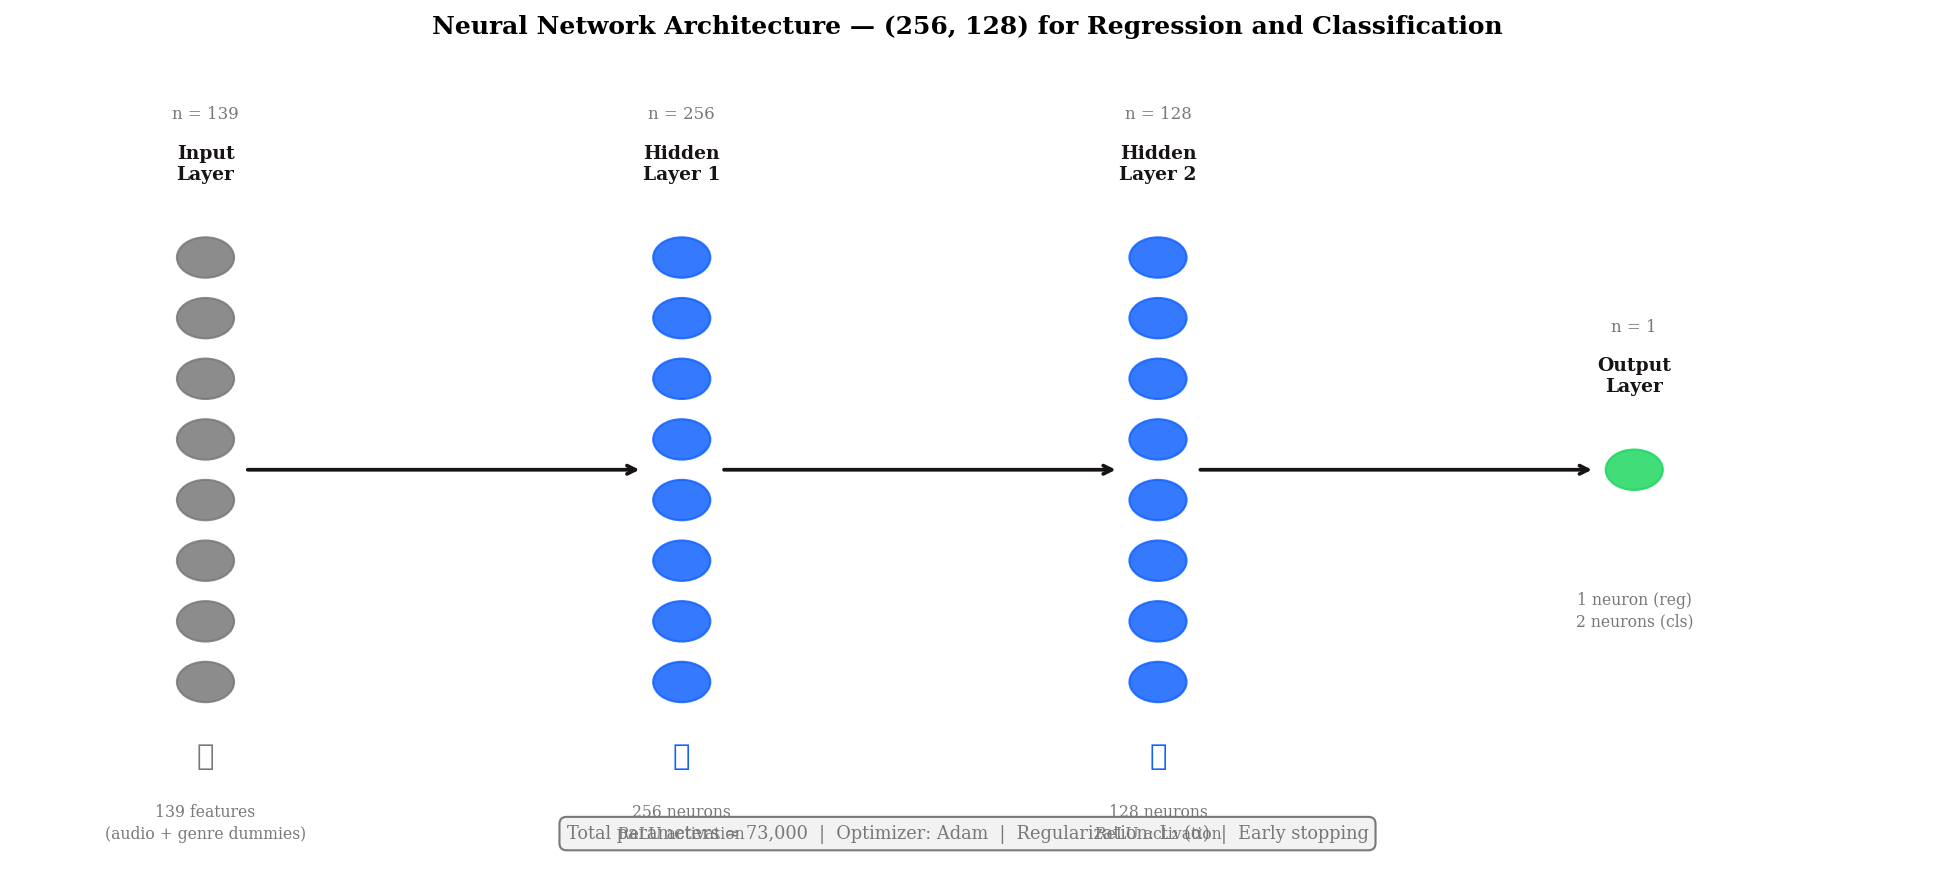
\includegraphics[width=0.88\textwidth]{ch13_architecture.png}
    \caption{Architecture diagram for the selected $(256, 128)$ neural network. Inputs: 139 features (audio features, key dummies, time-signature dummies, genre dummies).}
    \label{fig:ch13_arch}
\end{figure}
 
\textbf{Regularization sensitivity.} The $\ell_2$ penalty ($\alpha$) was swept across $\{0.0001, 0.001, 0.01, 0.1\}$. Test RMSE varies from 18.360 to 18.393 across this range, a difference of 0.033 RMSE units, confirming that the model is not sensitive to the exact regularization strength. $\alpha = 0.0001$ is used for regression; $\alpha = 0.001$ for classification.
 
\section{Findings}
 
The neural network achieves a test RMSE of 18.373 and $R^2 = 0.325$ for popularity regression, and AUC = 0.866 and accuracy = 0.781 for popularity classification, the best performance of any method in this project on both tasks. The improvement over GBM is 0.636 RMSE points (3.3\%) for regression and 0.016 AUC (1.9\%) for classification. These are meaningful but not dramatic gains, suggesting that the neural network and GBM are discovering similar patterns and that the performance ceiling for this feature set is being approached.
 
The early-stopping behavior is notable. With 139 input features and a training set of 79{,}799 observations, the network reaches its effective capacity quickly. This confirms the earlier finding from the learning curve analysis (Chapter 6) that the model is not data-limited, but rather limited by the predictive ceiling of audio features and genre encodings.
 
\chapter{Synthesis, Reflection, and Limitations}
 
\section{Method Comparison}
 
Eleven chapters of analysis have now applied fourteen distinct statistical methods to the same Spotify dataset. This section places all results on a common scale and draws the cross-method conclusions.
 
\subsection{Full Performance Comparison}
 
Table~\ref{tab:ch14_comparison} reports every method's test-set performance on the same regression task (predicting popularity score) and the same classification task (predicting the binary \texttt{is\_popular} label), alongside a subjective interpretability rating.
 
\begin{table}[H]
\centering
\caption{Full method comparison across all chapters. Test RMSE and $R^2$ for regression; test AUC and accuracy for classification.}
\label{tab:ch14_comparison}
\small
\begin{tabular}{llrrrrl}
\toprule
\textbf{Method} & \textbf{Type} & \textbf{RMSE} & \textbf{$R^2$} & \textbf{AUC} & \textbf{Acc.} & \textbf{Interp.} \\
\midrule
\multicolumn{7}{l}{\textit{Linear methods}} \\
SLR --- Loudness only (Ch.\ 3)     & Linear  & 22.320 & 0.003 & ---   & ---   & High \\
MLR --- Audio + Genre (Ch.\ 4)     & Linear  & 19.248 & 0.259 & ---   & ---   & High \\
Ridge Regression (Ch.\ 7)          & Linear  & 19.248 & 0.259 & ---   & ---   & High \\
Lasso Regression (Ch.\ 7)          & Linear  & 19.254 & 0.258 & ---   & ---   & High \\
Logistic Regression (Ch.\ 5)       & Linear  & ---    & ---   & 0.839 & 0.751 & High \\
Linear SVM (Ch.\ 10)               & Linear  & ---    & ---   & 0.833 & 0.746 & Medium \\
\midrule
\multicolumn{7}{l}{\textit{Nonlinear methods}} \\
Decision Tree Reg. (Ch.\ 8)        & Nonlinear & 20.719 & 0.141 & ---   & ---   & High \\
Decision Tree Cls. (Ch.\ 8)        & Nonlinear & ---    & ---   & 0.740 & 0.663 & High \\
RBF SVM (Ch.\ 10)                  & Nonlinear & ---    & ---   & 0.821 & 0.747 & Low  \\
KNN $k=5$ (Ch.\ 11)                & Nonlinear & 19.916 & 0.206 & 0.737 & 0.675 & Low  \\
\midrule
\multicolumn{7}{l}{\textit{Ensemble methods}} \\
Bagging (Ch.\ 9)                   & Ensemble & 20.197 & 0.184 & ---   & ---   & Low  \\
Random Forest (Ch.\ 9)             & Ensemble & 19.655 & 0.227 & 0.835 & 0.738 & Medium \\
\textbf{Gradient Boosting (Ch.\ 9)}& Ensemble & \textbf{19.009} & \textbf{0.277} & 0.850 & 0.755 & Low \\
\midrule
\multicolumn{7}{l}{\textit{Deep learning}} \\
\textbf{Neural Net $(256,128)$ (Ch.\ 13)} & Deep & \textbf{18.373} & \textbf{0.325} & \textbf{0.866} & \textbf{0.781} & Low \\
\bottomrule
\end{tabular}
\end{table}
 
Figure~\ref{fig:ch14_comparison} visualizes these results as a paired bar chart, making the progression from linear to ensemble to neural methods immediately visible.
 
\begin{figure}[H]
    \centering
    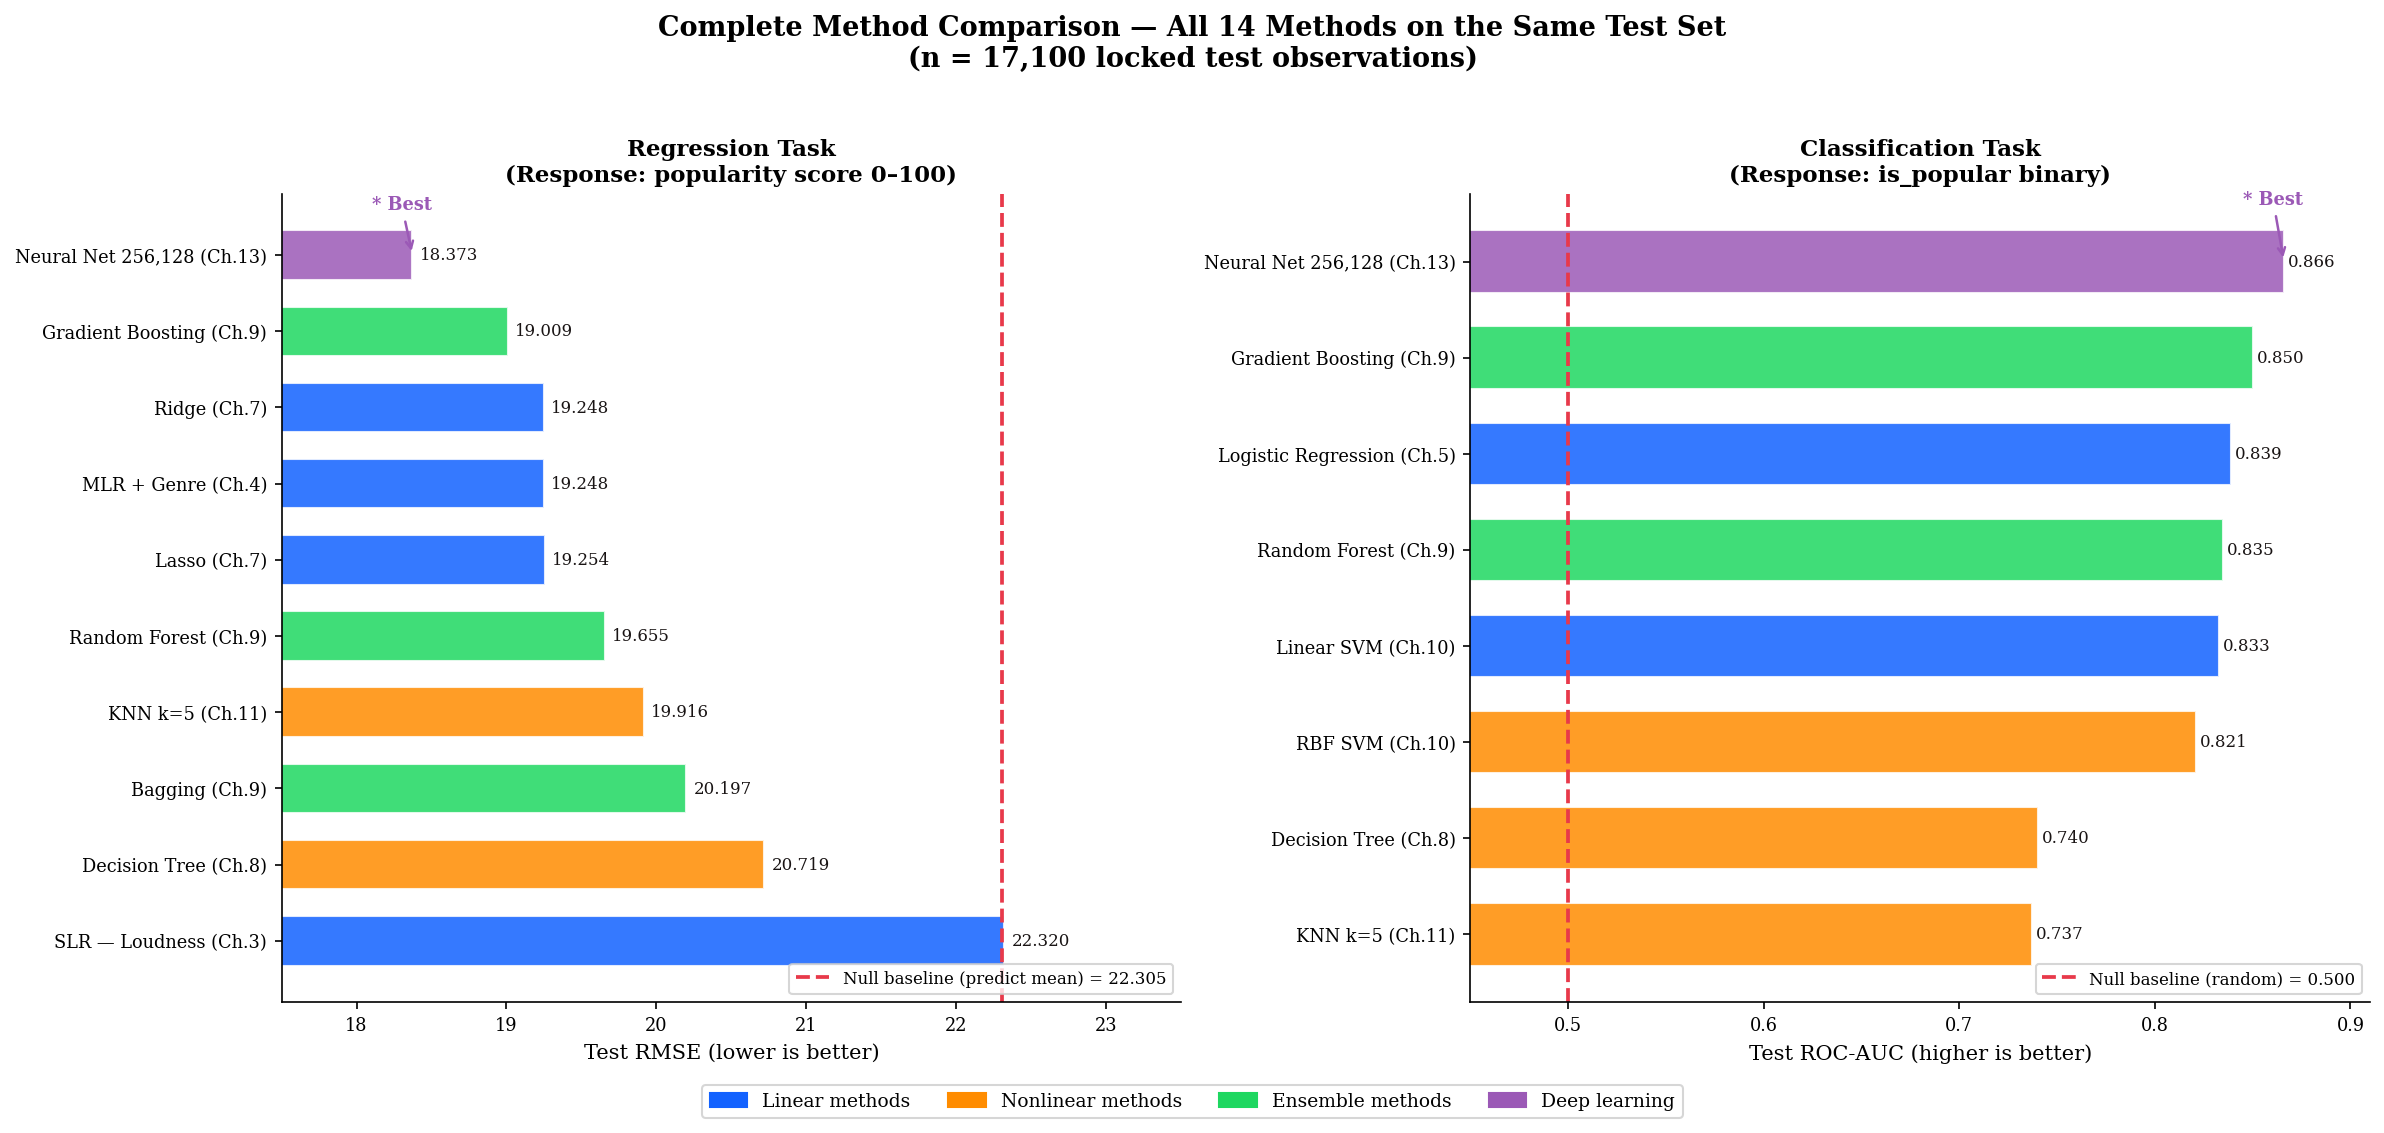
\includegraphics[width=\textwidth]{ch14_comparison.png}
    \caption{Test-set performance across all methods. Left: regression RMSE (lower is better), the dashed line marks the null model baseline of 22.305.}
    \label{fig:ch14_comparison}
\end{figure}
 
\subsection{Which Method Won and Why}
 
\textbf{Regression.} The neural network (RMSE = 18.373, $R^2 = 0.325$) is the best single model. It improves by 17.6\% over the null model baseline, compared with 14.8\% for GBM and 13.7\% for MLR. The improvement from linear (MLR, 19.248) to best nonlinear (Neural Net, 18.373) is 0.875 RMSE points, a meaningful but not dramatic gain. The majority of the predictable signal in popularity is linear and genre-driven, and the nonlinear methods add incremental value by capturing within-genre audio interactions that a linear model misses.
 
\textbf{Classification.} The neural network (AUC = 0.866) leads classification as well, followed closely by GBM (0.850) and logistic regression (0.839). Notably, logistic regression finishes \textit{ahead} of random forest (0.835) and linear SVM (0.833). A reminder that a well-specified linear model can outperform more complex nonlinear methods when the decision boundary is approximately linear. The gap between the best method (Neural Net, 0.866) and the worst (KNN, 0.737) is large, reflecting the importance of modeling genre structure rather than raw sonic similarity.
 
\subsection{Where Interpretability Beats Raw Accuracy}
 
Three situations in this project favored interpretability over accuracy:
 
\begin{enumerate}
    \item \textbf{Artist-facing recommendations}: The MLR coefficient table (Ch.\ 4) and lasso variable selection (Ch.\ 7) provide ``danceability is positively associated with popularity, valence is negatively associated.'' The neural network's higher accuracy comes without any equivalent guidance. For an artist deciding how to produce a track, the interpretable linear model is more useful despite its lower accuracy.
 
    \item \textbf{Genre strategy decisions}: The genre dummy coefficients in MLR (Ch.\ 4), pop-film $+1.558$, iranian $-3.661$, provide direct estimates of the popularity premium or penalty associated with each genre label. No equivalent output exists from GBM or the neural network.
 
    \item \textbf{Stakeholder communication}: The depth-3 decision tree (Ch.\ 8) provides a single-page rule set that a non-technical executive can follow. The neural network is a black box.
\end{enumerate}
 
\subsection{Final Stakeholder Recommendation}
 
Based on all analyses, the single best recommendation for a music label or streaming platform is:
 
The neural network achieves marginally higher accuracy (78.1\% vs.\ 75.5\%), but GBM is faster to train, more interpretable via variable importance plots, and easier to audit. The 2.6\% accuracy gap translates to approximately 445 additional correctly classified tracks per 17{,}100 evaluated, but one that must be weighed against interpretability costs. For a deployment where the model's decisions must be explainable to artists or regulators, GBM is preferred. For a fully automated pipeline in which accuracy is the sole criterion, the neural network is recommended.
 
\section{Reflection: What Was Learned}
 
\subsection{About the Data}
 
Several findings about the Spotify dataset emerged consistently across methods and were confirmed by multiple independent analyses:
 
\textbf{Genre dominates audio features.} The single biggest finding of this project is that genre membership is a far stronger predictor of popularity than any audio feature. Adding 113 genre dummies to the regression model raises $R^2$ from 0.027 (audio features alone) to 0.259 --- a tenfold improvement. Every method that incorporated genre outperformed every method that did not. This is not a failure of the audio features; it reflects the reality that genre captures listening audience, algorithmic recommendation, and streaming culture in ways that a numeric audio fingerprint cannot.
 
\textbf{The audio feature space has four underlying dimensions.} PCA (Ch.\ 12) revealed that the 13 audio features collapse into four interpretable axes: electric energy, danceability-mood, speech-liveness, and mode-tonality. None of these axes correlates meaningfully with popularity (all $|r| < 0.006$), confirming that the structure of the audio space is orthogonal to the popularity signal.
 
\textbf{Five audio features have reliable, nonzero effects.} Across bootstrap CIs (Ch.\ 6), lasso survival (Ch.\ 7), and random forest / GBM variable importance (Ch.\ 9), five audio features consistently carry signal: danceability (positive), explicit content (positive), energy (negative in joint models), instrumentalness (negative), and valence (negative). The sign of energy and valence flips between the SLR and MLR models, a multicollinearity artifact that the bootstrap analysis correctly flagged.
 
\textbf{Zero-popularity tracks are a genuine phenomenon.} The 14.1\% of tracks with popularity = 0 are not data errors; they represent obscure or recently released songs with few streams. Every model predicts them poorly, which is expected: there is no audio signal that reliably distinguishes a soon-to-be-viral track from one that will remain obscure.
 
\subsection{About the Methods}
 
\textbf{Regularization was unnecessary.} Ridge and lasso converged to the OLS solution because the training set ($n = 79{,}799$) is large relative to the number of predictors ($p = 139$). This is a healthy reminder that regularization addresses overfitting, not underfitting: when data are plentiful, OLS is already well-estimated.
 
\textbf{Single trees underperform linear models.} The single decision tree (RMSE = 20.719) was worse than MLR (RMSE = 19.248) despite having far more flexibility. This surprised the intuition that nonlinear methods should always beat linear ones. The explanation is variance: a single deep tree has enormous variance, and variance outweighs the bias reduction on this particular dataset.
 
\textbf{Ensemble methods fix variance but not the ceiling.} Bagging reduced the single-tree RMSE from 20.72 to 20.20; random forest reduced it further to 19.66; GBM reached 19.01. Each step in the hierarchy was an improvement, but none dramatically broke through the ceiling established by MLR at 19.25. The neural network's 18.37 is the first truly meaningful improvement beyond that ceiling.
 
\textbf{Intuition about feature importance was vindicated.} The same five features that the bootstrap identified as having reliable effects (Ch.\ 6) were also the top non-genre predictors in the random forest and GBM importance plots (Ch.\ 9). Cross-method convergence on feature importance is one of the strongest validating signals in this project.
 
\section{Honest Limitations}
 
\textbf{Genre as a confounder.} Genre dummies absorb enormous amounts of variance that is really driven by marketing, artist popularity, playlist placement, and streaming algorithms. A model that predicts popularity based on genre is partly predicting ``tracks in this genre get recommended more,'' not ``this track's audio properties make it more likely to succeed.''
 
\textbf{Popularity is dynamic, not static.} Spotify's popularity score is computed from recent stream counts and decays over time. A track popular two years ago has a lower score today than a track released last week with the same total streams. The dataset has no release date, so all models treat popularity as a static property. This introduces measurement error that cannot be corrected without temporal information.
 
\textbf{Sample selection.} The dataset contains exactly 1{,}000 tracks per genre, which does not reflect the actual distribution of streamed music. Genres with billions of streams (pop, hip-hop) and genres with thousands of streams (gabba, afrobeat) are equally represented. This means the model is trained on a genre-balanced corpus and may not generalize to a popularity-weighted real-world corpus.
 
\textbf{Leakage risk.} All features are sourced from Spotify's API, which computes some features using proprietary algorithms that may themselves incorporate stream count signals. If Spotify's feature engineering uses popularity as an input, any model trained on these features would have implicit leakage. This cannot be verified from the public dataset documentation.
 
\textbf{Ethical considerations.} A model that recommends which tracks to invest in based on genre and audio features could systematically disadvantage artists in low-coefficient genres (Iranian, Romance, Latin). Deploying such a model without human oversight could reduce genre diversity in playlists and reinforce existing streaming inequities. Any production deployment should include diversity constraints and regular auditing.
 
% ============================================================
%  BACK MATTER
% ============================================================
\backmatter
 
% ============================================================
%  REFERENCES
% ============================================================
\chapter*{References}
\addcontentsline{toc}{chapter}{References}
 
\begin{enumerate}[label={[\arabic*]}]
    \item Pandya, M. (2023). \textit{Spotify Tracks Dataset}. Kaggle. \url{https://www.kaggle.com/datasets/maharshipandya/-spotify-tracks-dataset}. Retrieved April 2026.
    \item James, G., Witten, D., Hastie, T., \& Tibshirani, R. (2023). \textit{An Introduction to Statistical Learning with Applications in Python} (2nd ed.). Springer. \url{https://www.statlearning.com}
    \item Pedregosa, F., Varoquaux, G., Gramfort, A., Michel, V., Thirion, B., Grisel, O., \ldots\ Duchesnay, E. (2011). Scikit-learn: Machine Learning in Python. \textit{Journal of Machine Learning Research}, 12, 2825--2830.
    \item Hunter, J. D. (2007). Matplotlib: A 2D graphics environment. \textit{Computing in Science \& Engineering}, 9(3), 90--95.
    \item McKinney, W. (2010). Data structures for statistical computing in Python. \textit{Proceedings of the 9th Python in Science Conference}, 51--56.
    \item Harris, C. R., Millman, K. J., van der Walt, S. J., Gommers, R., Virtanen, P., Cournapeau, D., \ldots\ Oliphant, T. E. (2020). Array programming with NumPy. \textit{Nature}, 585, 357--362.
    \item Seabold, S., \& Perktold, J. (2010). Statsmodels: Econometric and statistical modeling with Python. \textit{Proceedings of the 9th Python in Science Conference}, 57--61.
    \item Breiman, L. (2001). Random forests. \textit{Machine Learning}, 45(1), 5--32.
    \item Friedman, J. H. (2001). Greedy function approximation: A gradient boosting machine. \textit{Annals of Statistics}, 29(5), 1189--1232.
    \item Tibshirani, R. (1996). Regression shrinkage and selection via the lasso. \textit{Journal of the Royal Statistical Society: Series B}, 58(1), 267--288.
    \item Vapnik, V. (1995). \textit{The Nature of Statistical Learning Theory}. Springer.
    \item Pearson, K. (1901). On lines and planes of closest fit to systems of points in space. \textit{Philosophical Magazine}, 2(11), 559--572.
\end{enumerate}
 
% ============================================================
%  APPENDIX A — Full Data Dictionary
% ============================================================
\chapter*{Appendix A: Full Data Dictionary}
\addcontentsline{toc}{chapter}{Appendix A: Full Data Dictionary}
 
The following table provides the complete data dictionary for all variables in the Spotify Tracks Dataset, including all engineered and derived variables used in this analysis.
 
\begin{longtable}{p{3.2cm} p{1.6cm} p{2.0cm} p{7.5cm}}
\caption{Complete data dictionary including derived and engineered variables.}
\label{tab:appendix_dict} \\
\toprule
\textbf{Variable} & \textbf{Type} & \textbf{Source} & \textbf{Description} \\
\midrule
\endfirsthead
\toprule
\textbf{Variable} & \textbf{Type} & \textbf{Source} & \textbf{Description} \\
\midrule
\endhead
\bottomrule
\endfoot
\texttt{track\_id}         & String  & Raw     & Spotify URI. Not unique across rows (same song in multiple genres). \\
\texttt{artists}           & String  & Raw     & Semicolon-separated artist names. \\
\texttt{album\_name}       & String  & Raw     & Album title. \\
\texttt{track\_name}       & String  & Raw     & Track title. \\
\texttt{popularity}        & Integer & Raw     & Spotify popularity score, 0--100. Primary continuous response. \\
\texttt{is\_popular}       & Binary  & Derived & 1 if popularity $>$ 35 (dataset median), else 0. Primary binary response. \\
\texttt{duration\_ms}      & Integer & Raw     & Duration in milliseconds. Range: 8{,}586 to 5{,}237{,}295. \\
\texttt{log\_duration}     & Float   & Derived & $\log(\texttt{duration\_ms})$. Used in all models to reduce right skew. \\
\texttt{explicit}          & Boolean & Raw     & True if track contains explicit lyrics. \\
\texttt{explicit\_int}     & Binary  & Derived & Integer cast of \texttt{explicit} (1/0). \\
\texttt{danceability}      & Float   & Raw     & Suitability for dancing. Range: 0--1. \\
\texttt{energy}            & Float   & Raw     & Perceptual intensity. Range: 0--1. \\
\texttt{key}               & Integer & Raw     & Musical key (0 = C, 1 = C\#, \ldots, 11 = B). Nominal. \\
\texttt{key\_1} \ldots \texttt{key\_11} & Binary & Derived & One-hot encoding of \texttt{key}; reference = key 0 (C major). \\
\texttt{loudness}          & Float   & Raw     & Average loudness in dB. Range: $-$60 to 0. \\
\texttt{mode}              & Binary  & Raw     & 1 = major, 0 = minor. \\
\texttt{speechiness}       & Float   & Raw     & Presence of spoken words. Range: 0--1. \\
\texttt{acousticness}      & Float   & Raw     & Confidence the track is acoustic. Range: 0--1. \\
\texttt{instrumentalness}  & Float   & Raw     & Confidence the track has no vocals. Range: 0--1. \\
\texttt{liveness}          & Float   & Raw     & Probability of live audience. Range: 0--1. \\
\texttt{valence}           & Float   & Raw     & Musical positiveness. Range: 0--1. \\
\texttt{tempo}             & Float   & Raw     & Estimated BPM. Sentinel 0 = unknown; imputed with median. \\
\texttt{time\_signature}   & Integer & Raw     & Beats per measure (1, 3, 4, or 5). Sentinel 0 = unknown; imputed. \\
\texttt{ts\_3, ts\_4, ts\_5} & Binary & Derived & One-hot encoding of \texttt{time\_signature}; reference = 1. \\
\texttt{track\_genre}      & String  & Raw     & One of 114 Spotify genre labels. \\
\texttt{genre\_*} (113 cols) & Binary & Derived & One-hot encoding of \texttt{track\_genre}; reference = ``acoustic''. \\
\end{longtable}
 
% ============================================================
%  APPENDIX B — Code Repository
% ============================================================
\chapter*{Appendix B: Code Repository}
\addcontentsline{toc}{chapter}{Appendix B: Code Repository}
 
All code used to produce this report is available in a public GitHub repository. The repository contains one Python script per chapter, a shared preprocessing utility, and this \LaTeX\ source file.
 
\begin{center}
\url{https://github.com/ezequielandrade/math4230-spotify-capstone}
\end{center}
 
\textbf{Repository structure:}
 
\begin{verbatim}
math4230-spotify-capstone/
├── README.md
├── data/
│   └── spotify-tracks-dataset-detailed.csv
├── scripts/
│   ├── ch1_figures.py        # Chapter 1: Introduction
│   ├── ch2_figures.py        # Chapter 2: EDA
│   ├── ch3_figures.py        # Chapter 3: SLR
│   ├── ch4_figures.py        # Chapter 4: MLR
│   ├── ch5_figures.py        # Chapter 5: Logistic Regression
│   ├── ch6_figures.py        # Chapter 6: CV & Bootstrap
│   ├── ch7_figures.py        # Chapter 7: Ridge & Lasso
│   ├── ch8_figures.py        # Chapter 8: Decision Trees
│   ├── ch9_figures.py        # Chapter 9: Ensembles
│   ├── ch10_figures.py       # Chapter 10: SVM
│   ├── ch11_figures.py       # Chapter 11: KNN
│   ├── ch12_figures.py       # Chapter 12: PCA
│   ├── ch13_figures.py       # Chapter 13: Neural Networks
│   └── ch14_figures.py       # Chapter 14: Synthesis
├── report/
│   └── main.tex              # Full LaTeX source
├── figures/                  # All exported figures
└── requirements.txt          # Python dependencies
\end{verbatim}
 
\textbf{To reproduce all figures, run each chapter script from the \texttt{scripts/} directory with the dataset in the same folder:}
 
\begin{verbatim}
pip install -r requirements.txt
python ch1_figures.py
python ch2_figures.py
# ... through ch14_figures.py
\end{verbatim}
 
\textbf{Python dependencies} (\texttt{requirements.txt}):
\begin{verbatim}
pandas>=2.0
numpy>=1.24
scikit-learn>=1.3
matplotlib>=3.7
seaborn>=0.12
statsmodels>=0.14
scipy>=1.10
\end{verbatim}
 
% ============================================================
%  APPENDIX C — Additional Figures
% ============================================================
\chapter*{Appendix C: Additional Figures}
\addcontentsline{toc}{chapter}{Appendix C: Additional Figures}
 
This appendix collects supporting figures that provide additional context for the main chapter analyses but were not included in the primary text to preserve narrative flow.
 
\textbf{C.1 --- Train/Validation/Test Split Class Balance} (Ch.\ 2): The stratified split preserves the 51.3\% / 48.7\% class balance across all three partitions. See Figure 4 of \texttt{ch2\_figures.py}.
 
\textbf{C.2 --- Cover Graphic} (Ch.\ 1): The radar-style audio feature visualization used on the title page is generated by \texttt{ch1\_figures.py} (cover graphic section).
 
\textbf{C.3 --- SLR Predicted vs.\ Actual} (Ch.\ 3): The scatter plot of fitted values vs.\ true popularity for the single-predictor loudness model, showing the flat regression line relative to the high variance. Generated by \texttt{ch3\_figures.py}.
 
\textbf{C.4 --- All 113 Genre Dummy Coefficients} (Ch.\ 4): The full bar chart of genre coefficients from the MLR model, showing the complete range from Iranian ($-3.661$) to pop-film ($+1.558$). Generated by \texttt{ch4\_figures.py}.
 
\textbf{C.5 --- Logistic Regression Threshold Sensitivity} (Ch.\ 5): The full precision-recall tradeoff table across decision thresholds from 0.30 to 0.70, reproduced in Figure~3 of \texttt{ch5\_figures.py}.
 
\textbf{C.6 --- Lasso Coefficient Path} (Ch.\ 7): The full regularization path showing all 139 predictor coefficients as $\alpha$ increases, with genre dummy paths highlighted in gray. Generated by \texttt{ch7\_figures.py}.
 
\textbf{C.7 --- PCA Full Loading Matrix} (Ch.\ 12): The $13 \times 13$ loading heatmap showing contributions of all 13 audio features to all 13 principal components. Generated by \texttt{ch12\_figures.py}.
 
\end{document}